\documentclass{book}
\usepackage[a4paper,top=2.5cm,bottom=2.5cm,left=2.5cm,right=2.5cm]{geometry}
\usepackage{makeidx}
\usepackage{natbib}
\usepackage{graphicx}
\usepackage{multicol}
\usepackage{float}
\usepackage{listings}
\usepackage{color}
\usepackage{ifthen}
\usepackage[table]{xcolor}
\usepackage{textcomp}
\usepackage{alltt}
\usepackage{ifpdf}
\ifpdf
\usepackage[pdftex,
            pagebackref=true,
            colorlinks=true,
            linkcolor=blue,
            unicode
           ]{hyperref}
\else
\usepackage[ps2pdf,
            pagebackref=true,
            colorlinks=true,
            linkcolor=blue,
            unicode
           ]{hyperref}
\usepackage{pspicture}
\fi
\usepackage[utf8]{inputenc}
\usepackage{mathptmx}
\usepackage[scaled=.90]{helvet}
\usepackage{courier}
\usepackage{sectsty}
\usepackage{amssymb}
\usepackage[titles]{tocloft}
\usepackage{doxygen}
\lstset{language=C++,inputencoding=utf8,basicstyle=\footnotesize,breaklines=true,breakatwhitespace=true,tabsize=4,numbers=left }
\makeindex
\setcounter{tocdepth}{3}
\renewcommand{\footrulewidth}{0.4pt}
\renewcommand{\familydefault}{\sfdefault}
\hfuzz=15pt
\setlength{\emergencystretch}{15pt}
\hbadness=750
\tolerance=750
\begin{document}
\hypersetup{pageanchor=false,citecolor=blue}
\begin{titlepage}
\vspace*{7cm}
\begin{center}
{\Large Ba\-Ka\-Plan \\[1ex]\large Version 0.\-6 }\\
\vspace*{1cm}
{\large Generated by Doxygen 1.8.1.2}\\
\vspace*{0.5cm}
{\small Fri Feb 22 2013 22:56:30}\\
\end{center}
\end{titlepage}
\clearemptydoublepage
\pagenumbering{roman}
\tableofcontents
\clearemptydoublepage
\pagenumbering{arabic}
\hypersetup{pageanchor=true,citecolor=blue}
\chapter{Class Index}
\section{\-Class \-Hierarchy}
\-This inheritance list is sorted roughly, but not completely, alphabetically\-:\begin{DoxyCompactList}
\item \contentsline{section}{\-Database}{\pageref{de/d03/classDatabase}}{}
\item \contentsline{section}{\-Data\-Sheet}{\pageref{dd/dcc/classDataSheet}}{}
\item \contentsline{section}{\-Exapand\-Roll\-No}{\pageref{d2/d9b/classExapandRollNo}}{}
\item \contentsline{section}{\-Input\-Detail}{\pageref{db/d6e/classInputDetail}}{}
\begin{DoxyCompactList}
\item \contentsline{section}{\-Class\-Detail}{\pageref{d9/ddf/classClassDetail}}{}
\item \contentsline{section}{\-Date\-Sheet}{\pageref{de/d0e/classDateSheet}}{}
\item \contentsline{section}{\-Exam\-Detail}{\pageref{df/d4d/classExamDetail}}{}
\begin{DoxyCompactList}
\item \contentsline{section}{\-Valid\-Strategy}{\pageref{d9/d15/classValidStrategy}}{}
\end{DoxyCompactList}
\item \contentsline{section}{\-Login}{\pageref{dd/dfd/classLogin}}{}
\begin{DoxyCompactList}
\item \contentsline{section}{\-Project\-Detail}{\pageref{d3/dd8/classProjectDetail}}{}
\end{DoxyCompactList}
\item \contentsline{section}{\-Report}{\pageref{da/da8/classReport}}{}
\item \contentsline{section}{\-Roll\-No\-Detail}{\pageref{d6/db0/classRollNoDetail}}{}
\item \contentsline{section}{\-Room\-Detail}{\pageref{d4/de5/classRoomDetail}}{}
\item \contentsline{section}{\-Strategy}{\pageref{d2/df2/classStrategy}}{}
\end{DoxyCompactList}
\item \contentsline{section}{\-Input\-Field\-Name}{\pageref{dd/db2/classInputFieldName}}{}
\item \contentsline{section}{\-Java\-Script}{\pageref{da/dac/classJavaScript}}{}
\item \contentsline{section}{\-Page\-Structure\-Maker}{\pageref{de/d88/classPageStructureMaker}}{}
\begin{DoxyCompactList}
\item \contentsline{section}{\-Page\-Layout}{\pageref{d7/d9e/classPageLayout}}{}
\end{DoxyCompactList}
\item \contentsline{section}{\-Read\-Input}{\pageref{de/d50/classReadInput}}{}
\begin{DoxyCompactList}
\item \contentsline{section}{\-Arrange\-Roll\-No}{\pageref{da/de9/classArrangeRollNo}}{}
\begin{DoxyCompactList}
\item \contentsline{section}{\-Date\-Sheet}{\pageref{de/d0e/classDateSheet}}{}
\end{DoxyCompactList}
\item \contentsline{section}{\-Expand\-Roll\-No}{\pageref{d0/d6e/classExpandRollNo}}{}
\item \contentsline{section}{\-Seat\-Plan}{\pageref{d2/d41/classSeatPlan}}{}
\begin{DoxyCompactList}
\item \contentsline{section}{\-Strategy}{\pageref{d2/df2/classStrategy}}{}
\end{DoxyCompactList}
\end{DoxyCompactList}
\item \contentsline{section}{\-Read\-Input\-Field}{\pageref{d8/d37/classReadInputField}}{}
\item \contentsline{section}{\-Send\-Mail}{\pageref{d6/d66/classSendMail}}{}
\end{DoxyCompactList}

\chapter{Class Index}
\section{Class List}
Here are the classes, structs, unions and interfaces with brief descriptions\-:\begin{DoxyCompactList}
\item\contentsline{section}{\hyperlink{classArrangeRollNo}{Arrange\-Roll\-No} }{\pageref{classArrangeRollNo}}{}
\item\contentsline{section}{\hyperlink{classBranchDetails}{Branch\-Details} }{\pageref{classBranchDetails}}{}
\item\contentsline{section}{\hyperlink{classBranchReport}{Branch\-Report} }{\pageref{classBranchReport}}{}
\item\contentsline{section}{\hyperlink{classExamDetails}{Exam\-Details} }{\pageref{classExamDetails}}{}
\item\contentsline{section}{\hyperlink{classExapandRollNo}{Exapand\-Roll\-No} }{\pageref{classExapandRollNo}}{}
\item\contentsline{section}{\hyperlink{classHome}{Home} }{\pageref{classHome}}{}
\item\contentsline{section}{\hyperlink{classHomeCSS}{Home\-C\-S\-S} }{\pageref{classHomeCSS}}{}
\item\contentsline{section}{\hyperlink{classHTMLTags}{H\-T\-M\-L\-Tags} \\*Base class containong Basic Html Tags and methods }{\pageref{classHTMLTags}}{}
\item\contentsline{section}{\hyperlink{classReadBranchDetails}{Read\-Branch\-Details} }{\pageref{classReadBranchDetails}}{}
\item\contentsline{section}{\hyperlink{classReadExamDetails}{Read\-Exam\-Details} }{\pageref{classReadExamDetails}}{}
\item\contentsline{section}{\hyperlink{classReadInput}{Read\-Input} }{\pageref{classReadInput}}{}
\item\contentsline{section}{\hyperlink{classReadRollNoDetails}{Read\-Roll\-No\-Details} }{\pageref{classReadRollNoDetails}}{}
\item\contentsline{section}{\hyperlink{classReadRoomDetails}{Read\-Room\-Details} }{\pageref{classReadRoomDetails}}{}
\item\contentsline{section}{\hyperlink{classReport}{Report} }{\pageref{classReport}}{}
\item\contentsline{section}{\hyperlink{classRollNoDetails}{Roll\-No\-Details} }{\pageref{classRollNoDetails}}{}
\item\contentsline{section}{\hyperlink{classRoomDetails}{Room\-Details} }{\pageref{classRoomDetails}}{}
\item\contentsline{section}{\hyperlink{classRoomReport}{Room\-Report} }{\pageref{classRoomReport}}{}
\item\contentsline{section}{\hyperlink{classSeatPlan}{Seat\-Plan} }{\pageref{classSeatPlan}}{}
\item\contentsline{section}{\hyperlink{classStrategy}{Strategy} }{\pageref{classStrategy}}{}
\item\contentsline{section}{\hyperlink{classSubjectWiseRollNo}{Subject\-Wise\-Roll\-No} }{\pageref{classSubjectWiseRollNo}}{}
\item\contentsline{section}{\hyperlink{classValidation}{Validation} }{\pageref{classValidation}}{}
\end{DoxyCompactList}

\chapter{Class Documentation}
\hypertarget{classClassDetails}{\section{Class\-Details Class Reference}
\label{classClassDetails}\index{Class\-Details@{Class\-Details}}
}


{\ttfamily \#include $<$classdetails.\-h$>$}

Inheritance diagram for Class\-Details\-:\begin{figure}[H]
\begin{center}
\leavevmode
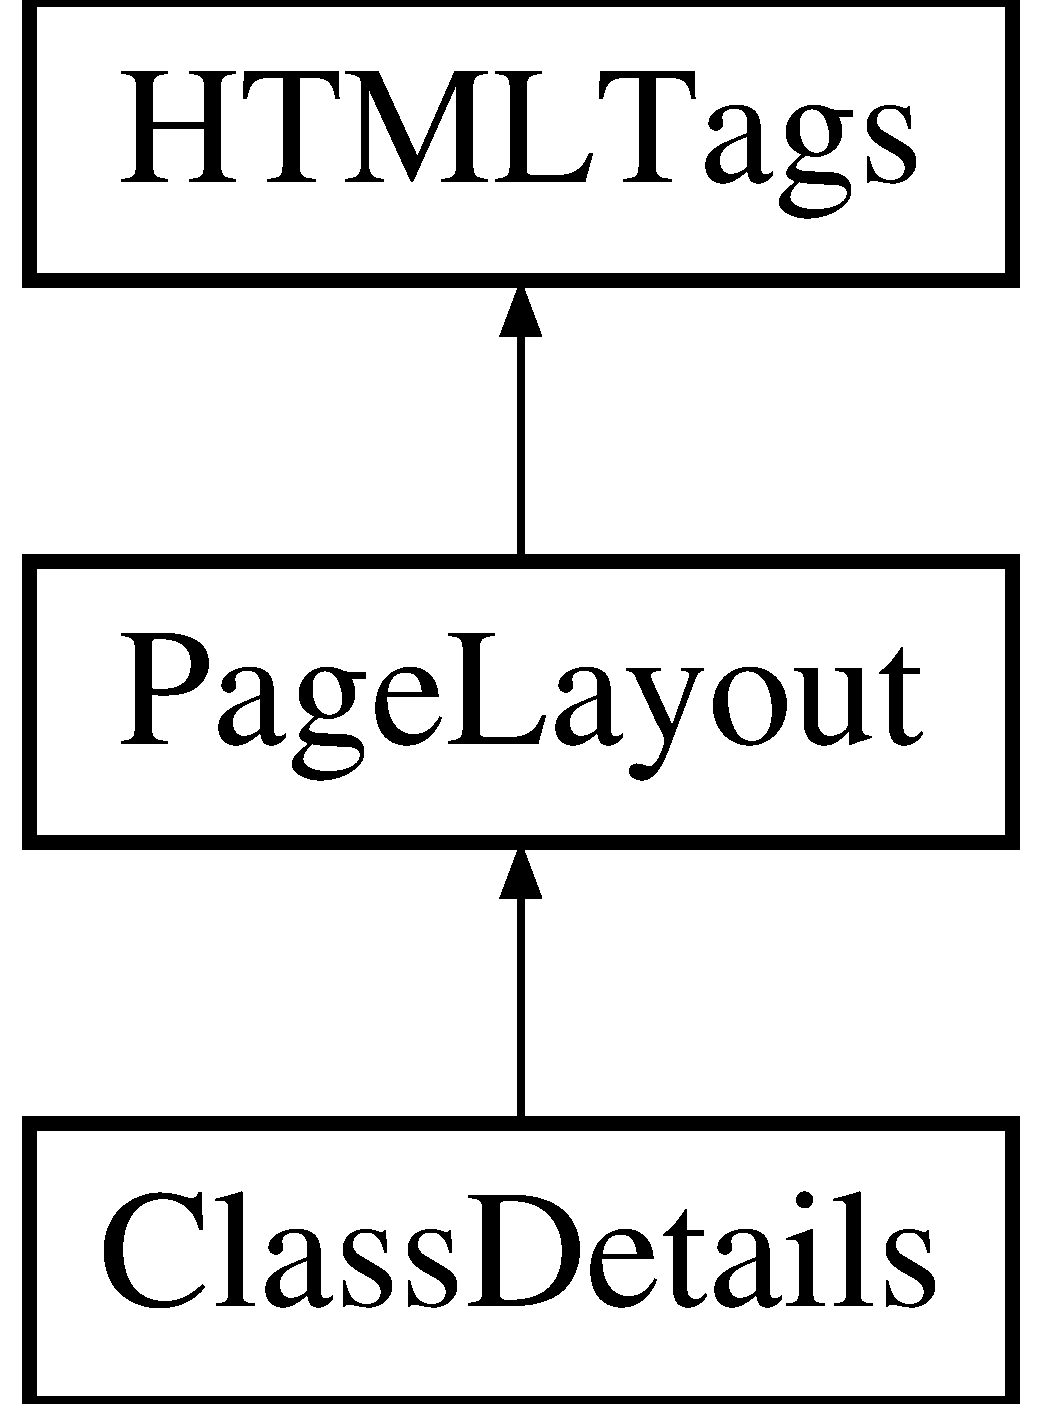
\includegraphics[height=3.000000cm]{classClassDetails}
\end{center}
\end{figure}
\subsection*{Public Member Functions}
\begin{DoxyCompactItemize}
\item 
\hyperlink{classClassDetails_af8fb7a92c63d62a03a60c47476f4523a}{Class\-Details} ()
\begin{DoxyCompactList}\small\item\em Constructor. \end{DoxyCompactList}\item 
void \hyperlink{classClassDetails_a2a63d68979d3ac96d35e6534414799ef}{Total\-Classes} ()
\begin{DoxyCompactList}\small\item\em Get total classes. \end{DoxyCompactList}\item 
void \hyperlink{classClassDetails_a7eed324cd736c68fe4b420de481e3b17}{Class\-Info} ()
\item 
void \hyperlink{classClassDetails_a4a0b14f8c5ca7f845d64854a0d81e1ec}{Header} ()
\begin{DoxyCompactList}\small\item\em Header of page. \end{DoxyCompactList}\item 
void \hyperlink{classClassDetails_a8e80a53e9b6597171c6d8b1976dc33f9}{Footer} ()
\begin{DoxyCompactList}\small\item\em Footer of page. \end{DoxyCompactList}\item 
void \hyperlink{classPageLayout_a49af1dca286bbee9432192a7b3c00332}{Menu} ()
\item 
void \hyperlink{classPageLayout_ae60235c6af48e3ebbc6343d02456da0c}{Logo} (string logo\-Name)
\item 
void \hyperlink{classPageLayout_ae50907d56f0ba7a85f7ccfdeafa45bcc}{Head} (string title\-Name)
\begin{DoxyCompactList}\small\item\em Head Section of Page. \end{DoxyCompactList}\item 
void \hyperlink{classHTMLTags_abe32ec84b6b2940afbc993be2db178e9}{Set\-H\-T\-M\-L\-Variables} ()
\begin{DoxyCompactList}\small\item\em Assingn Values to variables. \end{DoxyCompactList}\item 
void \hyperlink{classHTMLTags_a567551cd701d2836d4240b2917b5e13f}{H\-T\-M\-L\-Start} ()
\begin{DoxyCompactList}\small\item\em Display $<$\-H\-T\-M\-L$>$ \end{DoxyCompactList}\item 
void \hyperlink{classHTMLTags_a6553c3d01ee194a1d157e6341333dee3}{H\-T\-M\-L\-End} ()
\begin{DoxyCompactList}\small\item\em Display $<$/\-H\-T\-M\-L$>$ \end{DoxyCompactList}\item 
void \hyperlink{classHTMLTags_af2b01cc08884af52e0b291d07035062e}{Head\-Start} ()
\item 
void \hyperlink{classHTMLTags_afdc779e46fac16cc79e4f0e87f621254}{Head\-End} ()
\begin{DoxyCompactList}\small\item\em Display $<$/\-H\-E\-A\-D$>$ \end{DoxyCompactList}\item 
void \hyperlink{classHTMLTags_a5128d6f1c6be5ac1689047fc9d0d159f}{Title} (string page\-Title)
\begin{DoxyCompactList}\small\item\em Display $<$\-T\-I\-T\-L\-E$>$ $<$/\-T\-I\-T\-L\-E$>$ \end{DoxyCompactList}\item 
void \hyperlink{classHTMLTags_a4e9e18580cc7f2b82c82e4f81e39be50}{C\-S\-S} (string href)
\begin{DoxyCompactList}\small\item\em Add External C\-S\-S. \end{DoxyCompactList}\item 
void \hyperlink{classHTMLTags_aea041d720f12a210615c95350774e6aa}{Javascript} (string src)
\begin{DoxyCompactList}\small\item\em Add Javascript File. \end{DoxyCompactList}\item 
void \hyperlink{classHTMLTags_af1fb7b90b9ebb83177da18aba1ef86a9}{Body\-Start} ()
\begin{DoxyCompactList}\small\item\em Display $<$\-B\-O\-D\-Y$>$ \end{DoxyCompactList}\item 
void \hyperlink{classHTMLTags_a7cae36bd3a0e6f35e89494e5cda64971}{Body\-End} ()
\begin{DoxyCompactList}\small\item\em Display $<$/\-B\-O\-D\-Y$>$ \end{DoxyCompactList}\item 
void \hyperlink{classHTMLTags_a897512b202cfd12729e8fa24e67ea4d6}{Div\-Start} (string id, string class\-Name)
\begin{DoxyCompactList}\small\item\em Start Div Section. \end{DoxyCompactList}\item 
void \hyperlink{classHTMLTags_aa82b2d3d85b3afd29e5641dbe1ace439}{Div\-End} ()
\begin{DoxyCompactList}\small\item\em End div section. \end{DoxyCompactList}\item 
void \hyperlink{classHTMLTags_a1489ccf4629069eca5e550eeb8e8e887}{Form\-Start} (string name, string action, string method)
\begin{DoxyCompactList}\small\item\em Start Form. \end{DoxyCompactList}\item 
void \hyperlink{classHTMLTags_ab57baef28db9590ce59d0e2f403a210f}{Form\-End} ()
\begin{DoxyCompactList}\small\item\em End Form. \end{DoxyCompactList}\item 
void \hyperlink{classHTMLTags_a9d4bc37c7d615bc1d7f7c738dae48ad3}{Table\-Start} (string id, string class\-Name)
\begin{DoxyCompactList}\small\item\em Start Table. \end{DoxyCompactList}\item 
void \hyperlink{classHTMLTags_a0655d9f70a8c1a61c406280d8fb9df7a}{Table\-End} ()
\begin{DoxyCompactList}\small\item\em End Table. \end{DoxyCompactList}\item 
void \hyperlink{classHTMLTags_a705aef36f0847c2a5f10a5df8e079ce8}{Input\-Field} (string type, string name, int name\-No, string value)
\begin{DoxyCompactList}\small\item\em Input Field. \end{DoxyCompactList}\item 
void \hyperlink{classHTMLTags_adb6e7ef0a1320dbf6d4acbe1ea3e418f}{Select\-Field\-Start} (string name)
\begin{DoxyCompactList}\small\item\em Select Field Start. \end{DoxyCompactList}\item 
void \hyperlink{classHTMLTags_adde967a90e03f4b5168b9bffd319980b}{Select\-Field\-End} ()
\begin{DoxyCompactList}\small\item\em End Select Field. \end{DoxyCompactList}\item 
void \hyperlink{classHTMLTags_a372570979ccc675e0ed752fe272e3cd6}{Select\-Option\-Start} (string value, string selected)
\begin{DoxyCompactList}\small\item\em Select Option Start. \end{DoxyCompactList}\item 
void \hyperlink{classHTMLTags_ae312980d20e3dea0469fdcb730fb975e}{Select\-Option\-End} ()
\begin{DoxyCompactList}\small\item\em Selct Option End. \end{DoxyCompactList}\item 
void \hyperlink{classHTMLTags_ab6dbb027d808e7b708a4ece7e911ceee}{Button} (string id, string type, string class\-Name, string value)
\begin{DoxyCompactList}\small\item\em Button. \end{DoxyCompactList}\end{DoxyCompactItemize}
\subsection*{Protected Attributes}
\begin{DoxyCompactItemize}
\item 
\hypertarget{classClassDetails_a9bea81a0e09229c7060a592af6321b26}{int {\bfseries total\-Classes}}\label{classClassDetails_a9bea81a0e09229c7060a592af6321b26}

\item 
string {\bfseries class\-Name} \mbox{[}max\-Classes\mbox{]}
\item 
string {\bfseries subject\-Name} \mbox{[}max\-Classes\mbox{]}
\item 
string {\bfseries subject\-Code} \mbox{[}max\-Classes\mbox{]}
\item 
string {\bfseries table\-Heading} \mbox{[}4\mbox{]}
\item 
\hypertarget{classClassDetails_a53e447a55d35c02dcb02c6553380697e}{\hyperlink{classInputFieldNames}{Input\-Field\-Names} {\bfseries field\-Name}}\label{classClassDetails_a53e447a55d35c02dcb02c6553380697e}

\item 
\hypertarget{classClassDetails_a76dd2ba9e99ef8c24083a4b770003b07}{\hyperlink{classReadInputFields}{Read\-Input\-Fields} {\bfseries read\-Field}}\label{classClassDetails_a76dd2ba9e99ef8c24083a4b770003b07}

\item 
\hypertarget{classClassDetails_ab9f71f35c7f01ccbc4bfcd7e9f5ba28b}{int {\bfseries i}}\label{classClassDetails_ab9f71f35c7f01ccbc4bfcd7e9f5ba28b}

\item 
\hypertarget{classClassDetails_a57e44148f58db012a1cea587a09e2a4c}{int {\bfseries j}}\label{classClassDetails_a57e44148f58db012a1cea587a09e2a4c}

\item 
\hypertarget{classClassDetails_a1f87d306010f98019f49d965e15e8104}{int {\bfseries k}}\label{classClassDetails_a1f87d306010f98019f49d965e15e8104}

\item 
\hypertarget{classClassDetails_a0d3938ba9270a39f0579bd8fbe0cae0b}{stringstream {\bfseries ss}}\label{classClassDetails_a0d3938ba9270a39f0579bd8fbe0cae0b}

\item 
\hypertarget{classClassDetails_ade1a7d32883434c1a994c7c04a275d3d}{string {\bfseries temp}}\label{classClassDetails_ade1a7d32883434c1a994c7c04a275d3d}

\item 
string \hyperlink{classPageLayout_a8a3c1ddc422df2556fbc95d0cd575a05}{project\-Name}
\item 
\hypertarget{classPageLayout_a9abec89a54a6f0dac84114919d2ad117}{ifstream {\bfseries in\-File}}\label{classPageLayout_a9abec89a54a6f0dac84114919d2ad117}

\item 
\hypertarget{classPageLayout_ad52913274f786e82e1e09f5df4bf5347}{ofstream {\bfseries out\-File}}\label{classPageLayout_ad52913274f786e82e1e09f5df4bf5347}

\item 
string \hyperlink{classHTMLTags_ae987289d0dab2e3e234048615f930d0f}{start\-H1}
\begin{DoxyCompactList}\small\item\em H\-T\-M\-L Tag Variables for 

, , 

, etc. \end{DoxyCompactList}\item 
\hypertarget{classHTMLTags_a708194dea85c068a24b7923254fd7458}{string {\bfseries end\-H1}}\label{classHTMLTags_a708194dea85c068a24b7923254fd7458}

\item 
\hypertarget{classHTMLTags_a9290221d987dfe55acd3d2002a48efa0}{string {\bfseries start\-H3}}\label{classHTMLTags_a9290221d987dfe55acd3d2002a48efa0}

\item 
\hypertarget{classHTMLTags_afa471891c94946ba4a68acd727246d66}{string {\bfseries end\-H3}}\label{classHTMLTags_afa471891c94946ba4a68acd727246d66}

\item 
\hypertarget{classHTMLTags_a827d77a9a5cc3c442421420f0713c17a}{string {\bfseries start\-T\-D}}\label{classHTMLTags_a827d77a9a5cc3c442421420f0713c17a}

\item 
\hypertarget{classHTMLTags_ac2f4aae38f9d88d90df443e1e59a5bfc}{string {\bfseries end\-T\-D}}\label{classHTMLTags_ac2f4aae38f9d88d90df443e1e59a5bfc}

\item 
\hypertarget{classHTMLTags_a71b8a6e9593c6744f75fe8fac83e39b7}{string {\bfseries start\-T\-H}}\label{classHTMLTags_a71b8a6e9593c6744f75fe8fac83e39b7}

\item 
\hypertarget{classHTMLTags_a12cc718fee6ac4d701aafa9bc6303ad3}{string {\bfseries end\-T\-H}}\label{classHTMLTags_a12cc718fee6ac4d701aafa9bc6303ad3}

\item 
\hypertarget{classHTMLTags_ae8ee5ce9589d18b36263d62c6aa30e0a}{string {\bfseries start\-T\-R}}\label{classHTMLTags_ae8ee5ce9589d18b36263d62c6aa30e0a}

\item 
\hypertarget{classHTMLTags_ae6b79efff5ed7c253a050a6179057942}{string {\bfseries end\-T\-R}}\label{classHTMLTags_ae6b79efff5ed7c253a050a6179057942}

\item 
\hypertarget{classHTMLTags_ac6dafb63a2da3f7500cc080fd43a324d}{string {\bfseries start\-B}}\label{classHTMLTags_ac6dafb63a2da3f7500cc080fd43a324d}

\item 
\hypertarget{classHTMLTags_a12fc9d60d71c585cfba1643dc93eb8fc}{string {\bfseries end\-B}}\label{classHTMLTags_a12fc9d60d71c585cfba1643dc93eb8fc}

\item 
\hypertarget{classHTMLTags_a4403658fc74b6064bac61b0785ff0e85}{string {\bfseries brk}}\label{classHTMLTags_a4403658fc74b6064bac61b0785ff0e85}

\end{DoxyCompactItemize}


\subsection{Detailed Description}
=================================================================== Class\-: \hyperlink{classClassDetails}{Class\-Details} Description\-: This class is used to get details of class from \subsection*{user. Like class name, total classes, subject details etc.}

Definition at line 43 of file classdetails.\-h.



\subsection{Constructor \& Destructor Documentation}
\hypertarget{classClassDetails_af8fb7a92c63d62a03a60c47476f4523a}{\index{Class\-Details@{Class\-Details}!Class\-Details@{Class\-Details}}
\index{Class\-Details@{Class\-Details}!ClassDetails@{Class\-Details}}
\subsubsection[{Class\-Details}]{\setlength{\rightskip}{0pt plus 5cm}Class\-Details\-::\-Class\-Details (
\begin{DoxyParamCaption}
{}
\end{DoxyParamCaption}
)}}\label{classClassDetails_af8fb7a92c63d62a03a60c47476f4523a}


Constructor. 



 \subsubsection*{Incude header file which has \hyperlink{classClassDetails}{Class\-Details}'s declaration}

\subsubsection*{Defnition of member functions}



 Class\-: \hyperlink{classClassDetails}{Class\-Details} Method\-: \hyperlink{classClassDetails}{Class\-Details} \-:\-: \hyperlink{classClassDetails_af8fb7a92c63d62a03a60c47476f4523a}{Class\-Details()} \subsubsection*{Description\-: Constructor}

Definition at line 37 of file classdetails.\-cc.



\subsection{Member Function Documentation}
\hypertarget{classHTMLTags_a7cae36bd3a0e6f35e89494e5cda64971}{\index{Class\-Details@{Class\-Details}!Body\-End@{Body\-End}}
\index{Body\-End@{Body\-End}!ClassDetails@{Class\-Details}}
\subsubsection[{Body\-End}]{\setlength{\rightskip}{0pt plus 5cm}void H\-T\-M\-L\-Tags\-::\-Body\-End (
\begin{DoxyParamCaption}
{}
\end{DoxyParamCaption}
)\hspace{0.3cm}{\ttfamily [inherited]}}}\label{classHTMLTags_a7cae36bd3a0e6f35e89494e5cda64971}


Display $<$/\-B\-O\-D\-Y$>$ 



 Class\-: \hyperlink{classHTMLTags}{H\-T\-M\-L\-Tags} Method\-: \hyperlink{classHTMLTags}{H\-T\-M\-L\-Tags} \-:\-: \hyperlink{classHTMLTags_a7cae36bd3a0e6f35e89494e5cda64971}{Body\-End()} \subsubsection*{Description\-: Display }

Definition at line 180 of file htmltags.\-cc.

\hypertarget{classHTMLTags_af1fb7b90b9ebb83177da18aba1ef86a9}{\index{Class\-Details@{Class\-Details}!Body\-Start@{Body\-Start}}
\index{Body\-Start@{Body\-Start}!ClassDetails@{Class\-Details}}
\subsubsection[{Body\-Start}]{\setlength{\rightskip}{0pt plus 5cm}void H\-T\-M\-L\-Tags\-::\-Body\-Start (
\begin{DoxyParamCaption}
{}
\end{DoxyParamCaption}
)\hspace{0.3cm}{\ttfamily [inherited]}}}\label{classHTMLTags_af1fb7b90b9ebb83177da18aba1ef86a9}


Display $<$\-B\-O\-D\-Y$>$ 



 Class\-: \hyperlink{classHTMLTags}{H\-T\-M\-L\-Tags} Method\-: \hyperlink{classHTMLTags}{H\-T\-M\-L\-Tags} \-:\-: \hyperlink{classHTMLTags_af1fb7b90b9ebb83177da18aba1ef86a9}{Body\-Start()} \subsubsection*{Description\-: Display }

Definition at line 166 of file htmltags.\-cc.

\hypertarget{classHTMLTags_ab6dbb027d808e7b708a4ece7e911ceee}{\index{Class\-Details@{Class\-Details}!Button@{Button}}
\index{Button@{Button}!ClassDetails@{Class\-Details}}
\subsubsection[{Button}]{\setlength{\rightskip}{0pt plus 5cm}void H\-T\-M\-L\-Tags\-::\-Button (
\begin{DoxyParamCaption}
\item[{string}]{id, }
\item[{string}]{type, }
\item[{string}]{class\-Name, }
\item[{string}]{value}
\end{DoxyParamCaption}
)\hspace{0.3cm}{\ttfamily [inherited]}}}\label{classHTMLTags_ab6dbb027d808e7b708a4ece7e911ceee}


Button. 



 Class\-: \hyperlink{classHTMLTags}{H\-T\-M\-L\-Tags} Method\-: \hyperlink{classHTMLTags}{H\-T\-M\-L\-Tags} \-:\-: Button(string id, string type, string class\-Name, string value) \subsubsection*{Description\-: Create button(next, submit, etc)}

Definition at line 353 of file htmltags.\-cc.

\hypertarget{classClassDetails_a7eed324cd736c68fe4b420de481e3b17}{\index{Class\-Details@{Class\-Details}!Class\-Info@{Class\-Info}}
\index{Class\-Info@{Class\-Info}!ClassDetails@{Class\-Details}}
\subsubsection[{Class\-Info}]{\setlength{\rightskip}{0pt plus 5cm}void Class\-Details\-::\-Class\-Info (
\begin{DoxyParamCaption}
{}
\end{DoxyParamCaption}
)}}\label{classClassDetails_a7eed324cd736c68fe4b420de481e3b17}
Get class details like class name, subject name and subject code



 Class\-: \hyperlink{classClassDetails}{Class\-Details} Method\-: \hyperlink{classClassDetails}{Class\-Details} \-:\-: \hyperlink{classClassDetails_a7eed324cd736c68fe4b420de481e3b17}{Class\-Info()} Description\-: Get class name, subject code and subject name from \subsubsection*{user.}

Definition at line 148 of file classdetails.\-cc.

\hypertarget{classHTMLTags_a4e9e18580cc7f2b82c82e4f81e39be50}{\index{Class\-Details@{Class\-Details}!C\-S\-S@{C\-S\-S}}
\index{C\-S\-S@{C\-S\-S}!ClassDetails@{Class\-Details}}
\subsubsection[{C\-S\-S}]{\setlength{\rightskip}{0pt plus 5cm}void H\-T\-M\-L\-Tags\-::\-C\-S\-S (
\begin{DoxyParamCaption}
\item[{string}]{href}
\end{DoxyParamCaption}
)\hspace{0.3cm}{\ttfamily [inherited]}}}\label{classHTMLTags_a4e9e18580cc7f2b82c82e4f81e39be50}


Add External C\-S\-S. 



 Class\-: \hyperlink{classHTMLTags}{H\-T\-M\-L\-Tags} Method\-: \hyperlink{classHTMLTags}{H\-T\-M\-L\-Tags} \-:\-: \hyperlink{classHTMLTags_a4e9e18580cc7f2b82c82e4f81e39be50}{C\-S\-S(string href)} \subsubsection*{Description\-: Add External C\-S\-S file}

Definition at line 138 of file htmltags.\-cc.

\hypertarget{classHTMLTags_aa82b2d3d85b3afd29e5641dbe1ace439}{\index{Class\-Details@{Class\-Details}!Div\-End@{Div\-End}}
\index{Div\-End@{Div\-End}!ClassDetails@{Class\-Details}}
\subsubsection[{Div\-End}]{\setlength{\rightskip}{0pt plus 5cm}void H\-T\-M\-L\-Tags\-::\-Div\-End (
\begin{DoxyParamCaption}
{}
\end{DoxyParamCaption}
)\hspace{0.3cm}{\ttfamily [inherited]}}}\label{classHTMLTags_aa82b2d3d85b3afd29e5641dbe1ace439}


End div section. 



 Class\-: \hyperlink{classHTMLTags}{H\-T\-M\-L\-Tags} Method\-: \hyperlink{classHTMLTags}{H\-T\-M\-L\-Tags} \-:\-: \hyperlink{classHTMLTags_aa82b2d3d85b3afd29e5641dbe1ace439}{Div\-End()} \subsubsection*{Description\-: Close Div Section}

Definition at line 208 of file htmltags.\-cc.

\hypertarget{classHTMLTags_a897512b202cfd12729e8fa24e67ea4d6}{\index{Class\-Details@{Class\-Details}!Div\-Start@{Div\-Start}}
\index{Div\-Start@{Div\-Start}!ClassDetails@{Class\-Details}}
\subsubsection[{Div\-Start}]{\setlength{\rightskip}{0pt plus 5cm}void H\-T\-M\-L\-Tags\-::\-Div\-Start (
\begin{DoxyParamCaption}
\item[{string}]{id, }
\item[{string}]{class\-Name}
\end{DoxyParamCaption}
)\hspace{0.3cm}{\ttfamily [inherited]}}}\label{classHTMLTags_a897512b202cfd12729e8fa24e67ea4d6}


Start Div Section. 



 Class\-: \hyperlink{classHTMLTags}{H\-T\-M\-L\-Tags} Method\-: \hyperlink{classHTMLTags}{H\-T\-M\-L\-Tags} \-:\-: \hyperlink{classHTMLTags_a897512b202cfd12729e8fa24e67ea4d6}{Div\-Start(string id, string class\-Name)} \subsubsection*{Description\-: Start Div Section with id and class\-Name(for C\-S\-S)}

Definition at line 194 of file htmltags.\-cc.

\hypertarget{classClassDetails_a8e80a53e9b6597171c6d8b1976dc33f9}{\index{Class\-Details@{Class\-Details}!Footer@{Footer}}
\index{Footer@{Footer}!ClassDetails@{Class\-Details}}
\subsubsection[{Footer}]{\setlength{\rightskip}{0pt plus 5cm}void Class\-Details\-::\-Footer (
\begin{DoxyParamCaption}
{}
\end{DoxyParamCaption}
)}}\label{classClassDetails_a8e80a53e9b6597171c6d8b1976dc33f9}


Footer of page. 



 Class\-: \hyperlink{classClassDetails}{Class\-Details} Method\-: \hyperlink{classClassDetails}{Class\-Details} \-:\-: \hyperlink{classClassDetails_a8e80a53e9b6597171c6d8b1976dc33f9}{Footer()} \subsubsection*{Description\-: Footer of page}

Reimplemented from \hyperlink{classPageLayout_a68aa868a8868b12964f161838b5f814c}{Page\-Layout}.



Definition at line 89 of file classdetails.\-cc.

\hypertarget{classHTMLTags_ab57baef28db9590ce59d0e2f403a210f}{\index{Class\-Details@{Class\-Details}!Form\-End@{Form\-End}}
\index{Form\-End@{Form\-End}!ClassDetails@{Class\-Details}}
\subsubsection[{Form\-End}]{\setlength{\rightskip}{0pt plus 5cm}void H\-T\-M\-L\-Tags\-::\-Form\-End (
\begin{DoxyParamCaption}
{}
\end{DoxyParamCaption}
)\hspace{0.3cm}{\ttfamily [inherited]}}}\label{classHTMLTags_ab57baef28db9590ce59d0e2f403a210f}


End Form. 



 Class\-: \hyperlink{classHTMLTags}{H\-T\-M\-L\-Tags} Method\-: \hyperlink{classHTMLTags}{H\-T\-M\-L\-Tags} \-:\-: \hyperlink{classHTMLTags_ab57baef28db9590ce59d0e2f403a210f}{Form\-End()} \subsubsection*{Description\-: Close Form}

Definition at line 236 of file htmltags.\-cc.

\hypertarget{classHTMLTags_a1489ccf4629069eca5e550eeb8e8e887}{\index{Class\-Details@{Class\-Details}!Form\-Start@{Form\-Start}}
\index{Form\-Start@{Form\-Start}!ClassDetails@{Class\-Details}}
\subsubsection[{Form\-Start}]{\setlength{\rightskip}{0pt plus 5cm}void H\-T\-M\-L\-Tags\-::\-Form\-Start (
\begin{DoxyParamCaption}
\item[{string}]{name, }
\item[{string}]{action, }
\item[{string}]{method}
\end{DoxyParamCaption}
)\hspace{0.3cm}{\ttfamily [inherited]}}}\label{classHTMLTags_a1489ccf4629069eca5e550eeb8e8e887}


Start Form. 



 Class\-: \hyperlink{classHTMLTags}{H\-T\-M\-L\-Tags} Method\-: \hyperlink{classHTMLTags}{H\-T\-M\-L\-Tags} \-:\-: Form\-Start(string name, string action, string method) \subsubsection*{Description\-: Start Form with name, action and method(G\-E\-T/\-P\-O\-S\-T)}

Definition at line 222 of file htmltags.\-cc.

\hypertarget{classPageLayout_ae50907d56f0ba7a85f7ccfdeafa45bcc}{\index{Class\-Details@{Class\-Details}!Head@{Head}}
\index{Head@{Head}!ClassDetails@{Class\-Details}}
\subsubsection[{Head}]{\setlength{\rightskip}{0pt plus 5cm}void Page\-Layout\-::\-Head (
\begin{DoxyParamCaption}
\item[{string}]{title\-Name}
\end{DoxyParamCaption}
)\hspace{0.3cm}{\ttfamily [inherited]}}}\label{classPageLayout_ae50907d56f0ba7a85f7ccfdeafa45bcc}


Head Section of Page. 



 Class\-: \hyperlink{classPageLayout}{Page\-Layout} Method\-: \hyperlink{classPageLayout}{Page\-Layout} \-:\-: \hyperlink{classPageLayout_ae50907d56f0ba7a85f7ccfdeafa45bcc}{Head(string title\-Name)} Description\-: Head Section of page, titla\-Name pass to Title \subsubsection*{function.}

Definition at line 105 of file pagelayout.\-cc.

\hypertarget{classHTMLTags_afdc779e46fac16cc79e4f0e87f621254}{\index{Class\-Details@{Class\-Details}!Head\-End@{Head\-End}}
\index{Head\-End@{Head\-End}!ClassDetails@{Class\-Details}}
\subsubsection[{Head\-End}]{\setlength{\rightskip}{0pt plus 5cm}void H\-T\-M\-L\-Tags\-::\-Head\-End (
\begin{DoxyParamCaption}
{}
\end{DoxyParamCaption}
)\hspace{0.3cm}{\ttfamily [inherited]}}}\label{classHTMLTags_afdc779e46fac16cc79e4f0e87f621254}


Display $<$/\-H\-E\-A\-D$>$ 



 Class\-: \hyperlink{classHTMLTags}{H\-T\-M\-L\-Tags} Method\-: \hyperlink{classHTMLTags}{H\-T\-M\-L\-Tags} \-:\-: \hyperlink{classHTMLTags_afdc779e46fac16cc79e4f0e87f621254}{Head\-End()} \subsubsection*{Description\-: Display }

Definition at line 112 of file htmltags.\-cc.

\hypertarget{classClassDetails_a4a0b14f8c5ca7f845d64854a0d81e1ec}{\index{Class\-Details@{Class\-Details}!Header@{Header}}
\index{Header@{Header}!ClassDetails@{Class\-Details}}
\subsubsection[{Header}]{\setlength{\rightskip}{0pt plus 5cm}void Class\-Details\-::\-Header (
\begin{DoxyParamCaption}
{}
\end{DoxyParamCaption}
)}}\label{classClassDetails_a4a0b14f8c5ca7f845d64854a0d81e1ec}


Header of page. 



 Class\-: \hyperlink{classClassDetails}{Class\-Details} Method\-: \hyperlink{classClassDetails}{Class\-Details} \-:\-: \hyperlink{classClassDetails_a4a0b14f8c5ca7f845d64854a0d81e1ec}{Header()} \subsubsection*{Description\-: Includes menu, logo, header of page}

Reimplemented from \hyperlink{classPageLayout_a7726061f0653245f644a05807fa92472}{Page\-Layout}.



Definition at line 72 of file classdetails.\-cc.

\hypertarget{classHTMLTags_af2b01cc08884af52e0b291d07035062e}{\index{Class\-Details@{Class\-Details}!Head\-Start@{Head\-Start}}
\index{Head\-Start@{Head\-Start}!ClassDetails@{Class\-Details}}
\subsubsection[{Head\-Start}]{\setlength{\rightskip}{0pt plus 5cm}void H\-T\-M\-L\-Tags\-::\-Head\-Start (
\begin{DoxyParamCaption}
{}
\end{DoxyParamCaption}
)\hspace{0.3cm}{\ttfamily [inherited]}}}\label{classHTMLTags_af2b01cc08884af52e0b291d07035062e}


 Class\-: \hyperlink{classHTMLTags}{H\-T\-M\-L\-Tags} Method\-: \hyperlink{classHTMLTags}{H\-T\-M\-L\-Tags} \-:\-: \hyperlink{classHTMLTags_af2b01cc08884af52e0b291d07035062e}{Head\-Start()} \subsubsection*{Description\-: Display }

Definition at line 99 of file htmltags.\-cc.

\hypertarget{classHTMLTags_a6553c3d01ee194a1d157e6341333dee3}{\index{Class\-Details@{Class\-Details}!H\-T\-M\-L\-End@{H\-T\-M\-L\-End}}
\index{H\-T\-M\-L\-End@{H\-T\-M\-L\-End}!ClassDetails@{Class\-Details}}
\subsubsection[{H\-T\-M\-L\-End}]{\setlength{\rightskip}{0pt plus 5cm}void H\-T\-M\-L\-Tags\-::\-H\-T\-M\-L\-End (
\begin{DoxyParamCaption}
{}
\end{DoxyParamCaption}
)\hspace{0.3cm}{\ttfamily [inherited]}}}\label{classHTMLTags_a6553c3d01ee194a1d157e6341333dee3}


Display $<$/\-H\-T\-M\-L$>$ 



 Class\-: \hyperlink{classHTMLTags}{H\-T\-M\-L\-Tags} Method\-: \hyperlink{classHTMLTags}{H\-T\-M\-L\-Tags} \-:\-: \hyperlink{classHTMLTags_a6553c3d01ee194a1d157e6341333dee3}{H\-T\-M\-L\-End()} \subsubsection*{Description\-: Display }

Definition at line 86 of file htmltags.\-cc.

\hypertarget{classHTMLTags_a567551cd701d2836d4240b2917b5e13f}{\index{Class\-Details@{Class\-Details}!H\-T\-M\-L\-Start@{H\-T\-M\-L\-Start}}
\index{H\-T\-M\-L\-Start@{H\-T\-M\-L\-Start}!ClassDetails@{Class\-Details}}
\subsubsection[{H\-T\-M\-L\-Start}]{\setlength{\rightskip}{0pt plus 5cm}void H\-T\-M\-L\-Tags\-::\-H\-T\-M\-L\-Start (
\begin{DoxyParamCaption}
{}
\end{DoxyParamCaption}
)\hspace{0.3cm}{\ttfamily [inherited]}}}\label{classHTMLTags_a567551cd701d2836d4240b2917b5e13f}


Display $<$\-H\-T\-M\-L$>$ 



 Class\-: \hyperlink{classHTMLTags}{H\-T\-M\-L\-Tags} Method\-: \hyperlink{classHTMLTags}{H\-T\-M\-L\-Tags} \-:\-: \hyperlink{classHTMLTags_a567551cd701d2836d4240b2917b5e13f}{H\-T\-M\-L\-Start()} \subsubsection*{Description\-: Display  Tag }

Definition at line 73 of file htmltags.\-cc.

\hypertarget{classHTMLTags_a705aef36f0847c2a5f10a5df8e079ce8}{\index{Class\-Details@{Class\-Details}!Input\-Field@{Input\-Field}}
\index{Input\-Field@{Input\-Field}!ClassDetails@{Class\-Details}}
\subsubsection[{Input\-Field}]{\setlength{\rightskip}{0pt plus 5cm}void H\-T\-M\-L\-Tags\-::\-Input\-Field (
\begin{DoxyParamCaption}
\item[{string}]{type, }
\item[{string}]{name, }
\item[{int}]{name\-No, }
\item[{string}]{value}
\end{DoxyParamCaption}
)\hspace{0.3cm}{\ttfamily [inherited]}}}\label{classHTMLTags_a705aef36f0847c2a5f10a5df8e079ce8}


Input Field. 



 Class\-: \hyperlink{classHTMLTags}{H\-T\-M\-L\-Tags} Method\-: \hyperlink{classHTMLTags}{H\-T\-M\-L\-Tags} \-:\-: Input\-Field(string type, string name, string value) Description\-: Create Input fields like text field, submit \subsubsection*{button, etc.}

Definition at line 278 of file htmltags.\-cc.

\hypertarget{classHTMLTags_aea041d720f12a210615c95350774e6aa}{\index{Class\-Details@{Class\-Details}!Javascript@{Javascript}}
\index{Javascript@{Javascript}!ClassDetails@{Class\-Details}}
\subsubsection[{Javascript}]{\setlength{\rightskip}{0pt plus 5cm}void H\-T\-M\-L\-Tags\-::\-Javascript (
\begin{DoxyParamCaption}
\item[{string}]{src}
\end{DoxyParamCaption}
)\hspace{0.3cm}{\ttfamily [inherited]}}}\label{classHTMLTags_aea041d720f12a210615c95350774e6aa}


Add Javascript File. 



 Class\-: \hyperlink{classHTMLTags}{H\-T\-M\-L\-Tags} Method\-: \hyperlink{classHTMLTags}{H\-T\-M\-L\-Tags} \-:\-: \hyperlink{classHTMLTags_aea041d720f12a210615c95350774e6aa}{Javascript(string src)} \subsubsection*{Description\-: Add external Javascript file}

Definition at line 153 of file htmltags.\-cc.

\hypertarget{classPageLayout_ae60235c6af48e3ebbc6343d02456da0c}{\index{Class\-Details@{Class\-Details}!Logo@{Logo}}
\index{Logo@{Logo}!ClassDetails@{Class\-Details}}
\subsubsection[{Logo}]{\setlength{\rightskip}{0pt plus 5cm}void Page\-Layout\-::\-Logo (
\begin{DoxyParamCaption}
\item[{string}]{logo\-Name}
\end{DoxyParamCaption}
)\hspace{0.3cm}{\ttfamily [inherited]}}}\label{classPageLayout_ae60235c6af48e3ebbc6343d02456da0c}
Logo on Page



 Class\-: \hyperlink{classPageLayout}{Page\-Layout} Method\-: \hyperlink{classPageLayout}{Page\-Layout} \-:\-: \hyperlink{classPageLayout_ae60235c6af48e3ebbc6343d02456da0c}{Logo(string logo\-Name)} \subsubsection*{Description\-: Logo to project}

Definition at line 73 of file pagelayout.\-cc.

\hypertarget{classPageLayout_a49af1dca286bbee9432192a7b3c00332}{\index{Class\-Details@{Class\-Details}!Menu@{Menu}}
\index{Menu@{Menu}!ClassDetails@{Class\-Details}}
\subsubsection[{Menu}]{\setlength{\rightskip}{0pt plus 5cm}void Page\-Layout\-::\-Menu (
\begin{DoxyParamCaption}
{}
\end{DoxyParamCaption}
)\hspace{0.3cm}{\ttfamily [inherited]}}}\label{classPageLayout_a49af1dca286bbee9432192a7b3c00332}
List/\-Menu Navigation()



 Class\-: \hyperlink{classPageLayout}{Page\-Layout} Method\-: \hyperlink{classPageLayout}{Page\-Layout} \-:\-: \hyperlink{classPageLayout_a49af1dca286bbee9432192a7b3c00332}{Menu()} \subsubsection*{Description\-: Add Menu on pages(for navigation)}

Definition at line 50 of file pagelayout.\-cc.

\hypertarget{classHTMLTags_adde967a90e03f4b5168b9bffd319980b}{\index{Class\-Details@{Class\-Details}!Select\-Field\-End@{Select\-Field\-End}}
\index{Select\-Field\-End@{Select\-Field\-End}!ClassDetails@{Class\-Details}}
\subsubsection[{Select\-Field\-End}]{\setlength{\rightskip}{0pt plus 5cm}void H\-T\-M\-L\-Tags\-::\-Select\-Field\-End (
\begin{DoxyParamCaption}
{}
\end{DoxyParamCaption}
)\hspace{0.3cm}{\ttfamily [inherited]}}}\label{classHTMLTags_adde967a90e03f4b5168b9bffd319980b}


End Select Field. 



 Class\-: \hyperlink{classHTMLTags}{H\-T\-M\-L\-Tags} Method\-: \hyperlink{classHTMLTags}{H\-T\-M\-L\-Tags} \-:\-: \hyperlink{classHTMLTags_adde967a90e03f4b5168b9bffd319980b}{Select\-Field\-End()} \subsubsection*{Description\-: Close select field}

Definition at line 309 of file htmltags.\-cc.

\hypertarget{classHTMLTags_adb6e7ef0a1320dbf6d4acbe1ea3e418f}{\index{Class\-Details@{Class\-Details}!Select\-Field\-Start@{Select\-Field\-Start}}
\index{Select\-Field\-Start@{Select\-Field\-Start}!ClassDetails@{Class\-Details}}
\subsubsection[{Select\-Field\-Start}]{\setlength{\rightskip}{0pt plus 5cm}void H\-T\-M\-L\-Tags\-::\-Select\-Field\-Start (
\begin{DoxyParamCaption}
\item[{string}]{name}
\end{DoxyParamCaption}
)\hspace{0.3cm}{\ttfamily [inherited]}}}\label{classHTMLTags_adb6e7ef0a1320dbf6d4acbe1ea3e418f}


Select Field Start. 



 Class\-: \hyperlink{classHTMLTags}{H\-T\-M\-L\-Tags} Method\-: \hyperlink{classHTMLTags}{H\-T\-M\-L\-Tags} \-:\-: \hyperlink{classHTMLTags_adb6e7ef0a1320dbf6d4acbe1ea3e418f}{Select\-Field\-Start(string name)} \subsubsection*{Description\-: Create Select Field}

Definition at line 296 of file htmltags.\-cc.

\hypertarget{classHTMLTags_ae312980d20e3dea0469fdcb730fb975e}{\index{Class\-Details@{Class\-Details}!Select\-Option\-End@{Select\-Option\-End}}
\index{Select\-Option\-End@{Select\-Option\-End}!ClassDetails@{Class\-Details}}
\subsubsection[{Select\-Option\-End}]{\setlength{\rightskip}{0pt plus 5cm}void H\-T\-M\-L\-Tags\-::\-Select\-Option\-End (
\begin{DoxyParamCaption}
{}
\end{DoxyParamCaption}
)\hspace{0.3cm}{\ttfamily [inherited]}}}\label{classHTMLTags_ae312980d20e3dea0469fdcb730fb975e}


Selct Option End. 



 Class\-: \hyperlink{classHTMLTags}{H\-T\-M\-L\-Tags} Method\-: \hyperlink{classHTMLTags}{H\-T\-M\-L\-Tags} \-:\-: \hyperlink{classHTMLTags_ae312980d20e3dea0469fdcb730fb975e}{Select\-Option\-End()} \subsubsection*{Description\-: Close select option}

Definition at line 339 of file htmltags.\-cc.

\hypertarget{classHTMLTags_a372570979ccc675e0ed752fe272e3cd6}{\index{Class\-Details@{Class\-Details}!Select\-Option\-Start@{Select\-Option\-Start}}
\index{Select\-Option\-Start@{Select\-Option\-Start}!ClassDetails@{Class\-Details}}
\subsubsection[{Select\-Option\-Start}]{\setlength{\rightskip}{0pt plus 5cm}void H\-T\-M\-L\-Tags\-::\-Select\-Option\-Start (
\begin{DoxyParamCaption}
\item[{string}]{value, }
\item[{string}]{selected}
\end{DoxyParamCaption}
)\hspace{0.3cm}{\ttfamily [inherited]}}}\label{classHTMLTags_a372570979ccc675e0ed752fe272e3cd6}


Select Option Start. 



 Class\-: \hyperlink{classHTMLTags}{H\-T\-M\-L\-Tags} Method\-: \hyperlink{classHTMLTags}{H\-T\-M\-L\-Tags} \-:\-: Select\-Option\-Start(string value, string selected) \subsubsection*{Description\-: Options for select }

Definition at line 323 of file htmltags.\-cc.

\hypertarget{classHTMLTags_abe32ec84b6b2940afbc993be2db178e9}{\index{Class\-Details@{Class\-Details}!Set\-H\-T\-M\-L\-Variables@{Set\-H\-T\-M\-L\-Variables}}
\index{Set\-H\-T\-M\-L\-Variables@{Set\-H\-T\-M\-L\-Variables}!ClassDetails@{Class\-Details}}
\subsubsection[{Set\-H\-T\-M\-L\-Variables}]{\setlength{\rightskip}{0pt plus 5cm}void H\-T\-M\-L\-Tags\-::\-Set\-H\-T\-M\-L\-Variables (
\begin{DoxyParamCaption}
{}
\end{DoxyParamCaption}
)\hspace{0.3cm}{\ttfamily [inherited]}}}\label{classHTMLTags_abe32ec84b6b2940afbc993be2db178e9}


Assingn Values to variables. 



 Class\-: \hyperlink{classHTMLTags}{H\-T\-M\-L\-Tags} Method\-: \hyperlink{classHTMLTags}{H\-T\-M\-L\-Tags} \-:\-: \hyperlink{classHTMLTags_abe32ec84b6b2940afbc993be2db178e9}{Set\-H\-T\-M\-L\-Variables()} Description\-: Set values of common H\-T\-M\-L tags in respective \subsubsection*{variables.}

Definition at line 48 of file htmltags.\-cc.

\hypertarget{classHTMLTags_a0655d9f70a8c1a61c406280d8fb9df7a}{\index{Class\-Details@{Class\-Details}!Table\-End@{Table\-End}}
\index{Table\-End@{Table\-End}!ClassDetails@{Class\-Details}}
\subsubsection[{Table\-End}]{\setlength{\rightskip}{0pt plus 5cm}void H\-T\-M\-L\-Tags\-::\-Table\-End (
\begin{DoxyParamCaption}
{}
\end{DoxyParamCaption}
)\hspace{0.3cm}{\ttfamily [inherited]}}}\label{classHTMLTags_a0655d9f70a8c1a61c406280d8fb9df7a}


End Table. 



 Class\-: \hyperlink{classHTMLTags}{H\-T\-M\-L\-Tags} Method\-: \hyperlink{classHTMLTags}{H\-T\-M\-L\-Tags} \-:\-: \hyperlink{classHTMLTags_a0655d9f70a8c1a61c406280d8fb9df7a}{Table\-End()} \subsubsection*{Description\-: Close Table tag}

Definition at line 263 of file htmltags.\-cc.

\hypertarget{classHTMLTags_a9d4bc37c7d615bc1d7f7c738dae48ad3}{\index{Class\-Details@{Class\-Details}!Table\-Start@{Table\-Start}}
\index{Table\-Start@{Table\-Start}!ClassDetails@{Class\-Details}}
\subsubsection[{Table\-Start}]{\setlength{\rightskip}{0pt plus 5cm}void H\-T\-M\-L\-Tags\-::\-Table\-Start (
\begin{DoxyParamCaption}
\item[{string}]{id, }
\item[{string}]{class\-Name}
\end{DoxyParamCaption}
)\hspace{0.3cm}{\ttfamily [inherited]}}}\label{classHTMLTags_a9d4bc37c7d615bc1d7f7c738dae48ad3}


Start Table. 



 Class\-: \hyperlink{classHTMLTags}{H\-T\-M\-L\-Tags} Method\-: \hyperlink{classHTMLTags}{H\-T\-M\-L\-Tags} \-:\-: \hyperlink{classHTMLTags_a9d4bc37c7d615bc1d7f7c738dae48ad3}{Table\-Start(string id, string class\-Name)} \subsubsection*{Description\-: Start Table with id and class\-Name(\-C\-S\-S) attributes}

Definition at line 249 of file htmltags.\-cc.

\hypertarget{classHTMLTags_a5128d6f1c6be5ac1689047fc9d0d159f}{\index{Class\-Details@{Class\-Details}!Title@{Title}}
\index{Title@{Title}!ClassDetails@{Class\-Details}}
\subsubsection[{Title}]{\setlength{\rightskip}{0pt plus 5cm}void H\-T\-M\-L\-Tags\-::\-Title (
\begin{DoxyParamCaption}
\item[{string}]{page\-Title}
\end{DoxyParamCaption}
)\hspace{0.3cm}{\ttfamily [inherited]}}}\label{classHTMLTags_a5128d6f1c6be5ac1689047fc9d0d159f}


Display $<$\-T\-I\-T\-L\-E$>$ $<$/\-T\-I\-T\-L\-E$>$ 



 Class\-: \hyperlink{classHTMLTags}{H\-T\-M\-L\-Tags} Method\-: \hyperlink{classHTMLTags}{H\-T\-M\-L\-Tags} \-:\-: \hyperlink{classHTMLTags_a5128d6f1c6be5ac1689047fc9d0d159f}{Title(string page\-Title)} \subsubsection*{Description\-: Display Page Tile}

Definition at line 125 of file htmltags.\-cc.

\hypertarget{classClassDetails_a2a63d68979d3ac96d35e6534414799ef}{\index{Class\-Details@{Class\-Details}!Total\-Classes@{Total\-Classes}}
\index{Total\-Classes@{Total\-Classes}!ClassDetails@{Class\-Details}}
\subsubsection[{Total\-Classes}]{\setlength{\rightskip}{0pt plus 5cm}void Class\-Details\-::\-Total\-Classes (
\begin{DoxyParamCaption}
{}
\end{DoxyParamCaption}
)}}\label{classClassDetails_a2a63d68979d3ac96d35e6534414799ef}


Get total classes. 



 Class\-: \hyperlink{classClassDetails}{Class\-Details} Method\-: \hyperlink{classClassDetails}{Class\-Details} \-:\-: \hyperlink{classClassDetails_a2a63d68979d3ac96d35e6534414799ef}{Total\-Classes()} \subsubsection*{Description\-: Get Total classes from user}

Definition at line 103 of file classdetails.\-cc.



\subsection{Member Data Documentation}
\hypertarget{classClassDetails_a493e8ed1abcf67813875cff05c2a4543}{\index{Class\-Details@{Class\-Details}!class\-Name@{class\-Name}}
\index{class\-Name@{class\-Name}!ClassDetails@{Class\-Details}}
\subsubsection[{class\-Name}]{\setlength{\rightskip}{0pt plus 5cm}string Class\-Details\-::class\-Name\mbox{[}max\-Classes\mbox{]}\hspace{0.3cm}{\ttfamily [protected]}}}\label{classClassDetails_a493e8ed1abcf67813875cff05c2a4543}
{\bfseries Initial value\-:}
\begin{DoxyCode}
 \{\textcolor{stringliteral}{"Info. Tech."}, \textcolor{stringliteral}{"10th"}, 
                                        \textcolor{stringliteral}{"ECE"}, \textcolor{stringliteral}{"Mech. Engg."}, 
                                        \textcolor{stringliteral}{"Production Engg."}, 
                                        \textcolor{stringliteral}{"Electrical Engg."}, \textcolor{stringliteral}{"IT"},             
                                        \textcolor{stringliteral}{"Electronics Engg."}, 
                                        \textcolor{stringliteral}{"Comp. Sci. Engg."}, \textcolor{stringliteral}{"MBA"}\}
\end{DoxyCode}


Definition at line 54 of file classdetails.\-h.

\hypertarget{classPageLayout_a8a3c1ddc422df2556fbc95d0cd575a05}{\index{Class\-Details@{Class\-Details}!project\-Name@{project\-Name}}
\index{project\-Name@{project\-Name}!ClassDetails@{Class\-Details}}
\subsubsection[{project\-Name}]{\setlength{\rightskip}{0pt plus 5cm}string Page\-Layout\-::project\-Name\hspace{0.3cm}{\ttfamily [protected]}, {\ttfamily [inherited]}}}\label{classPageLayout_a8a3c1ddc422df2556fbc95d0cd575a05}
Project Name = Ba\-Ka\-Plan 

Definition at line 37 of file pagelayout.\-h.

\hypertarget{classHTMLTags_ae987289d0dab2e3e234048615f930d0f}{\index{Class\-Details@{Class\-Details}!start\-H1@{start\-H1}}
\index{start\-H1@{start\-H1}!ClassDetails@{Class\-Details}}
\subsubsection[{start\-H1}]{\setlength{\rightskip}{0pt plus 5cm}string H\-T\-M\-L\-Tags\-::start\-H1\hspace{0.3cm}{\ttfamily [protected]}, {\ttfamily [inherited]}}}\label{classHTMLTags_ae987289d0dab2e3e234048615f930d0f}


H\-T\-M\-L Tag Variables for 

, , 

, etc. 



Definition at line 38 of file htmltags.\-h.

\hypertarget{classClassDetails_aabb81b0797930602510f4531c875c6d1}{\index{Class\-Details@{Class\-Details}!subject\-Code@{subject\-Code}}
\index{subject\-Code@{subject\-Code}!ClassDetails@{Class\-Details}}
\subsubsection[{subject\-Code}]{\setlength{\rightskip}{0pt plus 5cm}string Class\-Details\-::subject\-Code\mbox{[}max\-Classes\mbox{]}\hspace{0.3cm}{\ttfamily [protected]}}}\label{classClassDetails_aabb81b0797930602510f4531c875c6d1}
{\bfseries Initial value\-:}
\begin{DoxyCode}
 \{\textcolor{stringliteral}{"IT-101, IT-102"}, 
                                          \textcolor{stringliteral}{"ME-10,CE-252"}, \textcolor{stringliteral}{"EVS, ED-10"}, 
                                          \textcolor{stringliteral}{"ED-10, IT-102"}, \textcolor{stringliteral}{"IT-102"}, 
                                          \textcolor{stringliteral}{"IT-203"}, \textcolor{stringliteral}{"CE-120"}, \textcolor{stringliteral}{"ME-140"}, 
                                          \textcolor{stringliteral}{"EE-109, 1234S, IT-203"},    
                                          \textcolor{stringliteral}{"ME-101,ME-501,IT-101"} \}
\end{DoxyCode}


Definition at line 67 of file classdetails.\-h.

\hypertarget{classClassDetails_a24cb6f1543b6a13e6308594903f0d7ab}{\index{Class\-Details@{Class\-Details}!subject\-Name@{subject\-Name}}
\index{subject\-Name@{subject\-Name}!ClassDetails@{Class\-Details}}
\subsubsection[{subject\-Name}]{\setlength{\rightskip}{0pt plus 5cm}string Class\-Details\-::subject\-Name\mbox{[}max\-Classes\mbox{]}\hspace{0.3cm}{\ttfamily [protected]}}}\label{classClassDetails_a24cb6f1543b6a13e6308594903f0d7ab}
{\bfseries Initial value\-:}
\begin{DoxyCode}
 \{\textcolor{stringliteral}{"DBMS, SAD"}, \textcolor{stringliteral}{"Maths,Physics"},
                                          \textcolor{stringliteral}{"OS, EVS"}, \textcolor{stringliteral}{"Java, C++"}, \textcolor{stringliteral}{"EVS"},
                                          \textcolor{stringliteral}{"Chem."}, \textcolor{stringliteral}{"ED"}, \textcolor{stringliteral}{"Maths"},       
                                          \textcolor{stringliteral}{"Maths,DBMS, Physics"},
                                          \textcolor{stringliteral}{"Multimedia, Dot Net, ED"}\}
\end{DoxyCode}


Definition at line 61 of file classdetails.\-h.

\hypertarget{classClassDetails_a0f5d73651bbf0ea0919cb6a2993c2afc}{\index{Class\-Details@{Class\-Details}!table\-Heading@{table\-Heading}}
\index{table\-Heading@{table\-Heading}!ClassDetails@{Class\-Details}}
\subsubsection[{table\-Heading}]{\setlength{\rightskip}{0pt plus 5cm}string Class\-Details\-::table\-Heading\mbox{[}4\mbox{]}\hspace{0.3cm}{\ttfamily [protected]}}}\label{classClassDetails_a0f5d73651bbf0ea0919cb6a2993c2afc}
{\bfseries Initial value\-:}
\begin{DoxyCode}
 \{\textcolor{stringliteral}{"Class Name"}, \textcolor{stringliteral}{"Total Subjects"}, 
                                  \textcolor{stringliteral}{"Subject Name"}, \textcolor{stringliteral}{"Subject Code"}\}
\end{DoxyCode}


Definition at line 74 of file classdetails.\-h.



The documentation for this class was generated from the following files\-:\begin{DoxyCompactItemize}
\item 
src/classdetails.\-h\item 
src/classdetails.\-cc\end{DoxyCompactItemize}

\hypertarget{classHTMLTags}{\section{H\-T\-M\-L\-Tags Class Reference}
\label{classHTMLTags}\index{H\-T\-M\-L\-Tags@{H\-T\-M\-L\-Tags}}
}


{\ttfamily \#include $<$htmltags.\-h$>$}

Inheritance diagram for H\-T\-M\-L\-Tags\-:\begin{figure}[H]
\begin{center}
\leavevmode
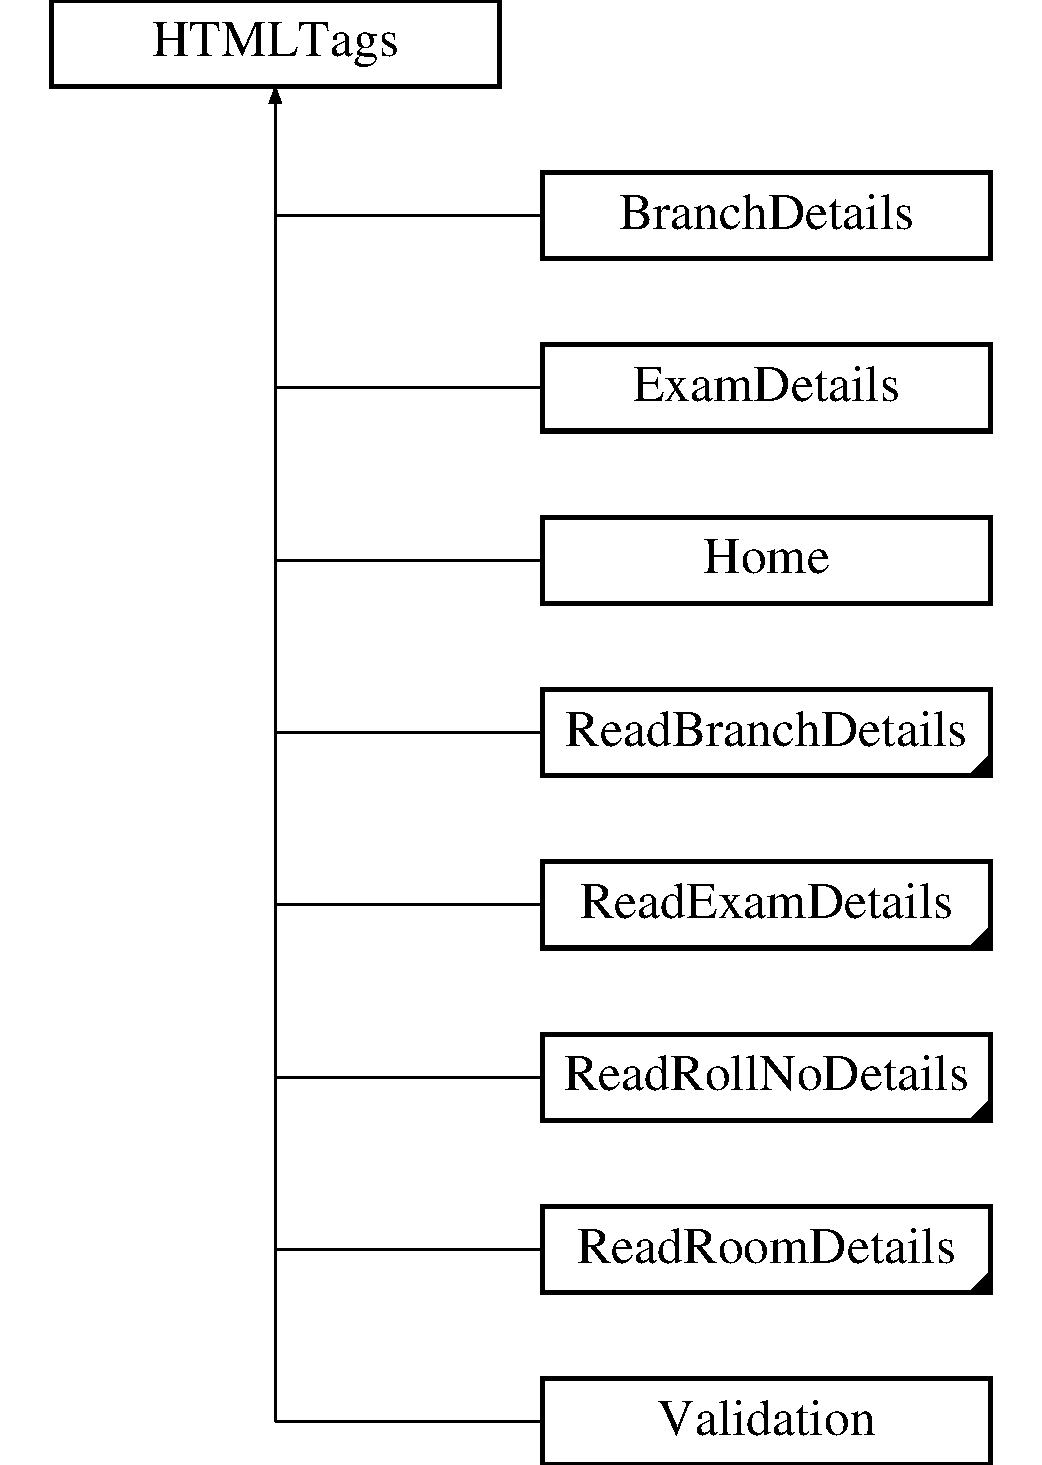
\includegraphics[height=3.000000cm]{classHTMLTags}
\end{center}
\end{figure}
\subsection*{Public Member Functions}
\begin{DoxyCompactItemize}
\item 
\hyperlink{classHTMLTags_a4f0bb4f538b87033b574ff05798eb60b}{H\-T\-M\-L\-Tags} ()
\begin{DoxyCompactList}\small\item\em Constructor. \end{DoxyCompactList}\item 
void \hyperlink{classHTMLTags_abe32ec84b6b2940afbc993be2db178e9}{Set\-H\-T\-M\-L\-Variables} ()
\begin{DoxyCompactList}\small\item\em Assingn Values to variables. \end{DoxyCompactList}\item 
void \hyperlink{classHTMLTags_a567551cd701d2836d4240b2917b5e13f}{H\-T\-M\-L\-Start} ()
\begin{DoxyCompactList}\small\item\em Display $<$\-H\-T\-M\-L$>$ \end{DoxyCompactList}\item 
void \hyperlink{classHTMLTags_a6553c3d01ee194a1d157e6341333dee3}{H\-T\-M\-L\-End} ()
\begin{DoxyCompactList}\small\item\em Display $<$/\-H\-T\-M\-L$>$ \end{DoxyCompactList}\item 
void \hyperlink{classHTMLTags_af2b01cc08884af52e0b291d07035062e}{Head\-Start} ()
\item 
void \hyperlink{classHTMLTags_afdc779e46fac16cc79e4f0e87f621254}{Head\-End} ()
\begin{DoxyCompactList}\small\item\em Display $<$/\-H\-E\-A\-D$>$ \end{DoxyCompactList}\item 
void \hyperlink{classHTMLTags_a5128d6f1c6be5ac1689047fc9d0d159f}{Title} (string page\-Title)
\begin{DoxyCompactList}\small\item\em Display $<$\-T\-I\-T\-L\-E$>$ $<$/\-T\-I\-T\-L\-E$>$ \end{DoxyCompactList}\item 
void \hyperlink{classHTMLTags_a4e9e18580cc7f2b82c82e4f81e39be50}{C\-S\-S} (string href)
\begin{DoxyCompactList}\small\item\em Add External C\-S\-S. \end{DoxyCompactList}\item 
void \hyperlink{classHTMLTags_aea041d720f12a210615c95350774e6aa}{Javascript} (string src)
\begin{DoxyCompactList}\small\item\em Add Javascript File. \end{DoxyCompactList}\item 
void \hyperlink{classHTMLTags_af1fb7b90b9ebb83177da18aba1ef86a9}{Body\-Start} ()
\begin{DoxyCompactList}\small\item\em Display $<$\-B\-O\-D\-Y$>$ \end{DoxyCompactList}\item 
void \hyperlink{classHTMLTags_a7cae36bd3a0e6f35e89494e5cda64971}{Body\-End} ()
\begin{DoxyCompactList}\small\item\em Display $<$/\-B\-O\-D\-Y$>$ \end{DoxyCompactList}\item 
void \hyperlink{classHTMLTags_a897512b202cfd12729e8fa24e67ea4d6}{Div\-Start} (string id, string class\-Name)
\begin{DoxyCompactList}\small\item\em Start Div Section. \end{DoxyCompactList}\item 
void \hyperlink{classHTMLTags_aa82b2d3d85b3afd29e5641dbe1ace439}{Div\-End} ()
\begin{DoxyCompactList}\small\item\em End div section. \end{DoxyCompactList}\item 
void \hyperlink{classHTMLTags_a1489ccf4629069eca5e550eeb8e8e887}{Form\-Start} (string name, string action, string method)
\begin{DoxyCompactList}\small\item\em Start Form. \end{DoxyCompactList}\item 
void \hyperlink{classHTMLTags_ab57baef28db9590ce59d0e2f403a210f}{Form\-End} ()
\begin{DoxyCompactList}\small\item\em End Form. \end{DoxyCompactList}\item 
void \hyperlink{classHTMLTags_a9d4bc37c7d615bc1d7f7c738dae48ad3}{Table\-Start} (string id, string class\-Name)
\begin{DoxyCompactList}\small\item\em Start Table. \end{DoxyCompactList}\item 
void \hyperlink{classHTMLTags_a0655d9f70a8c1a61c406280d8fb9df7a}{Table\-End} ()
\begin{DoxyCompactList}\small\item\em End Table. \end{DoxyCompactList}\item 
void \hyperlink{classHTMLTags_ab515d13346f63b00f7696374e682344e}{Input\-Field} (string type, string name, string value)
\begin{DoxyCompactList}\small\item\em Input Field. \end{DoxyCompactList}\item 
void \hyperlink{classHTMLTags_adb6e7ef0a1320dbf6d4acbe1ea3e418f}{Select\-Field\-Start} (string name)
\begin{DoxyCompactList}\small\item\em Select Field Start. \end{DoxyCompactList}\item 
void \hyperlink{classHTMLTags_adde967a90e03f4b5168b9bffd319980b}{Select\-Field\-End} ()
\begin{DoxyCompactList}\small\item\em End Select Field. \end{DoxyCompactList}\item 
void \hyperlink{classHTMLTags_a09f91c8601aed3aa2d0978123225afaa}{Select\-Option\-Start} (string value)
\begin{DoxyCompactList}\small\item\em Select Option Start. \end{DoxyCompactList}\item 
void \hyperlink{classHTMLTags_ae312980d20e3dea0469fdcb730fb975e}{Select\-Option\-End} ()
\begin{DoxyCompactList}\small\item\em Selct Option End. \end{DoxyCompactList}\item 
void \hyperlink{classHTMLTags_ab6dbb027d808e7b708a4ece7e911ceee}{Button} (string id, string type, string class\-Name, string value)
\begin{DoxyCompactList}\small\item\em Button. \end{DoxyCompactList}\end{DoxyCompactItemize}
\subsection*{Protected Attributes}
\begin{DoxyCompactItemize}
\item 
string \hyperlink{classHTMLTags_ae987289d0dab2e3e234048615f930d0f}{start\-H1}
\begin{DoxyCompactList}\small\item\em H\-T\-M\-L Tag Variables for 

, , 

, etc. \end{DoxyCompactList}\item 
\hypertarget{classHTMLTags_a708194dea85c068a24b7923254fd7458}{string {\bfseries end\-H1}}\label{classHTMLTags_a708194dea85c068a24b7923254fd7458}

\item 
\hypertarget{classHTMLTags_a9290221d987dfe55acd3d2002a48efa0}{string {\bfseries start\-H3}}\label{classHTMLTags_a9290221d987dfe55acd3d2002a48efa0}

\item 
\hypertarget{classHTMLTags_afa471891c94946ba4a68acd727246d66}{string {\bfseries end\-H3}}\label{classHTMLTags_afa471891c94946ba4a68acd727246d66}

\item 
\hypertarget{classHTMLTags_a827d77a9a5cc3c442421420f0713c17a}{string {\bfseries start\-T\-D}}\label{classHTMLTags_a827d77a9a5cc3c442421420f0713c17a}

\item 
\hypertarget{classHTMLTags_ac2f4aae38f9d88d90df443e1e59a5bfc}{string {\bfseries end\-T\-D}}\label{classHTMLTags_ac2f4aae38f9d88d90df443e1e59a5bfc}

\item 
\hypertarget{classHTMLTags_a71b8a6e9593c6744f75fe8fac83e39b7}{string {\bfseries start\-T\-H}}\label{classHTMLTags_a71b8a6e9593c6744f75fe8fac83e39b7}

\item 
\hypertarget{classHTMLTags_a12cc718fee6ac4d701aafa9bc6303ad3}{string {\bfseries end\-T\-H}}\label{classHTMLTags_a12cc718fee6ac4d701aafa9bc6303ad3}

\item 
\hypertarget{classHTMLTags_ae8ee5ce9589d18b36263d62c6aa30e0a}{string {\bfseries start\-T\-R}}\label{classHTMLTags_ae8ee5ce9589d18b36263d62c6aa30e0a}

\item 
\hypertarget{classHTMLTags_ae6b79efff5ed7c253a050a6179057942}{string {\bfseries end\-T\-R}}\label{classHTMLTags_ae6b79efff5ed7c253a050a6179057942}

\item 
\hypertarget{classHTMLTags_ac6dafb63a2da3f7500cc080fd43a324d}{string {\bfseries start\-B}}\label{classHTMLTags_ac6dafb63a2da3f7500cc080fd43a324d}

\item 
\hypertarget{classHTMLTags_a12fc9d60d71c585cfba1643dc93eb8fc}{string {\bfseries end\-B}}\label{classHTMLTags_a12fc9d60d71c585cfba1643dc93eb8fc}

\end{DoxyCompactItemize}


\subsection{Detailed Description}
\subsection*{Include Header file }

Class\-: \hyperlink{classHTMLTags}{H\-T\-M\-L\-Tags} \subsection*{Description\-: Declaration}

Definition at line 30 of file htmltags.\-h.



\subsection{Constructor \& Destructor Documentation}
\hypertarget{classHTMLTags_a4f0bb4f538b87033b574ff05798eb60b}{\index{H\-T\-M\-L\-Tags@{H\-T\-M\-L\-Tags}!H\-T\-M\-L\-Tags@{H\-T\-M\-L\-Tags}}
\index{H\-T\-M\-L\-Tags@{H\-T\-M\-L\-Tags}!HTMLTags@{H\-T\-M\-L\-Tags}}
\subsubsection[{H\-T\-M\-L\-Tags}]{\setlength{\rightskip}{0pt plus 5cm}H\-T\-M\-L\-Tags\-::\-H\-T\-M\-L\-Tags (
\begin{DoxyParamCaption}
{}
\end{DoxyParamCaption}
)}}\label{classHTMLTags_a4f0bb4f538b87033b574ff05798eb60b}


Constructor. 



 Class\-: \hyperlink{classHTMLTags}{H\-T\-M\-L\-Tags} Method\-: \hyperlink{classHTMLTags}{H\-T\-M\-L\-Tags} \-:\-: \hyperlink{classHTMLTags_a4f0bb4f538b87033b574ff05798eb60b}{H\-T\-M\-L\-Tags()} \subsubsection*{Description\-: Constructor}

Definition at line 27 of file htmltags.\-cc.



\subsection{Member Function Documentation}
\hypertarget{classHTMLTags_a7cae36bd3a0e6f35e89494e5cda64971}{\index{H\-T\-M\-L\-Tags@{H\-T\-M\-L\-Tags}!Body\-End@{Body\-End}}
\index{Body\-End@{Body\-End}!HTMLTags@{H\-T\-M\-L\-Tags}}
\subsubsection[{Body\-End}]{\setlength{\rightskip}{0pt plus 5cm}void H\-T\-M\-L\-Tags\-::\-Body\-End (
\begin{DoxyParamCaption}
{}
\end{DoxyParamCaption}
)}}\label{classHTMLTags_a7cae36bd3a0e6f35e89494e5cda64971}


Display $<$/\-B\-O\-D\-Y$>$ 



 Class\-: \hyperlink{classHTMLTags}{H\-T\-M\-L\-Tags} Method\-: \hyperlink{classHTMLTags}{H\-T\-M\-L\-Tags} \-:\-: \hyperlink{classHTMLTags_a7cae36bd3a0e6f35e89494e5cda64971}{Body\-End()} \subsubsection*{Description\-: Display }

Definition at line 172 of file htmltags.\-cc.

\hypertarget{classHTMLTags_af1fb7b90b9ebb83177da18aba1ef86a9}{\index{H\-T\-M\-L\-Tags@{H\-T\-M\-L\-Tags}!Body\-Start@{Body\-Start}}
\index{Body\-Start@{Body\-Start}!HTMLTags@{H\-T\-M\-L\-Tags}}
\subsubsection[{Body\-Start}]{\setlength{\rightskip}{0pt plus 5cm}void H\-T\-M\-L\-Tags\-::\-Body\-Start (
\begin{DoxyParamCaption}
{}
\end{DoxyParamCaption}
)}}\label{classHTMLTags_af1fb7b90b9ebb83177da18aba1ef86a9}


Display $<$\-B\-O\-D\-Y$>$ 



 Class\-: \hyperlink{classHTMLTags}{H\-T\-M\-L\-Tags} Method\-: \hyperlink{classHTMLTags}{H\-T\-M\-L\-Tags} \-:\-: \hyperlink{classHTMLTags_af1fb7b90b9ebb83177da18aba1ef86a9}{Body\-Start()} \subsubsection*{Description\-: Display }

Definition at line 159 of file htmltags.\-cc.

\hypertarget{classHTMLTags_ab6dbb027d808e7b708a4ece7e911ceee}{\index{H\-T\-M\-L\-Tags@{H\-T\-M\-L\-Tags}!Button@{Button}}
\index{Button@{Button}!HTMLTags@{H\-T\-M\-L\-Tags}}
\subsubsection[{Button}]{\setlength{\rightskip}{0pt plus 5cm}void H\-T\-M\-L\-Tags\-::\-Button (
\begin{DoxyParamCaption}
\item[{string}]{id, }
\item[{string}]{type, }
\item[{string}]{class\-Name, }
\item[{string}]{value}
\end{DoxyParamCaption}
)}}\label{classHTMLTags_ab6dbb027d808e7b708a4ece7e911ceee}


Button. 



 Class\-: \hyperlink{classHTMLTags}{H\-T\-M\-L\-Tags} Method\-: \hyperlink{classHTMLTags}{H\-T\-M\-L\-Tags} \-:\-: Button(string id, string type, string class\-Name, string value) \subsubsection*{Description\-: Create button(next, submit, etc)}

Definition at line 340 of file htmltags.\-cc.

\hypertarget{classHTMLTags_a4e9e18580cc7f2b82c82e4f81e39be50}{\index{H\-T\-M\-L\-Tags@{H\-T\-M\-L\-Tags}!C\-S\-S@{C\-S\-S}}
\index{C\-S\-S@{C\-S\-S}!HTMLTags@{H\-T\-M\-L\-Tags}}
\subsubsection[{C\-S\-S}]{\setlength{\rightskip}{0pt plus 5cm}void H\-T\-M\-L\-Tags\-::\-C\-S\-S (
\begin{DoxyParamCaption}
\item[{string}]{href}
\end{DoxyParamCaption}
)}}\label{classHTMLTags_a4e9e18580cc7f2b82c82e4f81e39be50}


Add External C\-S\-S. 



 Class\-: \hyperlink{classHTMLTags}{H\-T\-M\-L\-Tags} Method\-: \hyperlink{classHTMLTags}{H\-T\-M\-L\-Tags} \-:\-: \hyperlink{classHTMLTags_a4e9e18580cc7f2b82c82e4f81e39be50}{C\-S\-S(string href)} \subsubsection*{Description\-: Add External C\-S\-S file}

Definition at line 131 of file htmltags.\-cc.

\hypertarget{classHTMLTags_aa82b2d3d85b3afd29e5641dbe1ace439}{\index{H\-T\-M\-L\-Tags@{H\-T\-M\-L\-Tags}!Div\-End@{Div\-End}}
\index{Div\-End@{Div\-End}!HTMLTags@{H\-T\-M\-L\-Tags}}
\subsubsection[{Div\-End}]{\setlength{\rightskip}{0pt plus 5cm}void H\-T\-M\-L\-Tags\-::\-Div\-End (
\begin{DoxyParamCaption}
{}
\end{DoxyParamCaption}
)}}\label{classHTMLTags_aa82b2d3d85b3afd29e5641dbe1ace439}


End div section. 



 Class\-: \hyperlink{classHTMLTags}{H\-T\-M\-L\-Tags} Method\-: \hyperlink{classHTMLTags}{H\-T\-M\-L\-Tags} \-:\-: \hyperlink{classHTMLTags_aa82b2d3d85b3afd29e5641dbe1ace439}{Div\-End()} \subsubsection*{Description\-: Close Div Section}

Definition at line 199 of file htmltags.\-cc.

\hypertarget{classHTMLTags_a897512b202cfd12729e8fa24e67ea4d6}{\index{H\-T\-M\-L\-Tags@{H\-T\-M\-L\-Tags}!Div\-Start@{Div\-Start}}
\index{Div\-Start@{Div\-Start}!HTMLTags@{H\-T\-M\-L\-Tags}}
\subsubsection[{Div\-Start}]{\setlength{\rightskip}{0pt plus 5cm}void H\-T\-M\-L\-Tags\-::\-Div\-Start (
\begin{DoxyParamCaption}
\item[{string}]{id, }
\item[{string}]{class\-Name}
\end{DoxyParamCaption}
)}}\label{classHTMLTags_a897512b202cfd12729e8fa24e67ea4d6}


Start Div Section. 



 Class\-: \hyperlink{classHTMLTags}{H\-T\-M\-L\-Tags} Method\-: \hyperlink{classHTMLTags}{H\-T\-M\-L\-Tags} \-:\-: \hyperlink{classHTMLTags_a897512b202cfd12729e8fa24e67ea4d6}{Div\-Start(string id, string class\-Name)} \subsubsection*{Description\-: Start Div Section with id and class\-Name(for C\-S\-S)}

Definition at line 185 of file htmltags.\-cc.

\hypertarget{classHTMLTags_ab57baef28db9590ce59d0e2f403a210f}{\index{H\-T\-M\-L\-Tags@{H\-T\-M\-L\-Tags}!Form\-End@{Form\-End}}
\index{Form\-End@{Form\-End}!HTMLTags@{H\-T\-M\-L\-Tags}}
\subsubsection[{Form\-End}]{\setlength{\rightskip}{0pt plus 5cm}void H\-T\-M\-L\-Tags\-::\-Form\-End (
\begin{DoxyParamCaption}
{}
\end{DoxyParamCaption}
)}}\label{classHTMLTags_ab57baef28db9590ce59d0e2f403a210f}


End Form. 



 Class\-: \hyperlink{classHTMLTags}{H\-T\-M\-L\-Tags} Method\-: \hyperlink{classHTMLTags}{H\-T\-M\-L\-Tags} \-:\-: \hyperlink{classHTMLTags_ab57baef28db9590ce59d0e2f403a210f}{Form\-End()} \subsubsection*{Description\-: Close Form}

Definition at line 227 of file htmltags.\-cc.

\hypertarget{classHTMLTags_a1489ccf4629069eca5e550eeb8e8e887}{\index{H\-T\-M\-L\-Tags@{H\-T\-M\-L\-Tags}!Form\-Start@{Form\-Start}}
\index{Form\-Start@{Form\-Start}!HTMLTags@{H\-T\-M\-L\-Tags}}
\subsubsection[{Form\-Start}]{\setlength{\rightskip}{0pt plus 5cm}void H\-T\-M\-L\-Tags\-::\-Form\-Start (
\begin{DoxyParamCaption}
\item[{string}]{name, }
\item[{string}]{action, }
\item[{string}]{method}
\end{DoxyParamCaption}
)}}\label{classHTMLTags_a1489ccf4629069eca5e550eeb8e8e887}


Start Form. 



 Class\-: \hyperlink{classHTMLTags}{H\-T\-M\-L\-Tags} Method\-: \hyperlink{classHTMLTags}{H\-T\-M\-L\-Tags} \-:\-: Form\-Start(string name, string action, string method) \subsubsection*{Description\-: Start Form with name, action and method(G\-E\-T/\-P\-O\-S\-T)}

Definition at line 213 of file htmltags.\-cc.

\hypertarget{classHTMLTags_afdc779e46fac16cc79e4f0e87f621254}{\index{H\-T\-M\-L\-Tags@{H\-T\-M\-L\-Tags}!Head\-End@{Head\-End}}
\index{Head\-End@{Head\-End}!HTMLTags@{H\-T\-M\-L\-Tags}}
\subsubsection[{Head\-End}]{\setlength{\rightskip}{0pt plus 5cm}void H\-T\-M\-L\-Tags\-::\-Head\-End (
\begin{DoxyParamCaption}
{}
\end{DoxyParamCaption}
)}}\label{classHTMLTags_afdc779e46fac16cc79e4f0e87f621254}


Display $<$/\-H\-E\-A\-D$>$ 



 Class\-: \hyperlink{classHTMLTags}{H\-T\-M\-L\-Tags} Method\-: \hyperlink{classHTMLTags}{H\-T\-M\-L\-Tags} \-:\-: \hyperlink{classHTMLTags_afdc779e46fac16cc79e4f0e87f621254}{Head\-End()} \subsubsection*{Description\-: Display }

Definition at line 105 of file htmltags.\-cc.

\hypertarget{classHTMLTags_af2b01cc08884af52e0b291d07035062e}{\index{H\-T\-M\-L\-Tags@{H\-T\-M\-L\-Tags}!Head\-Start@{Head\-Start}}
\index{Head\-Start@{Head\-Start}!HTMLTags@{H\-T\-M\-L\-Tags}}
\subsubsection[{Head\-Start}]{\setlength{\rightskip}{0pt plus 5cm}void H\-T\-M\-L\-Tags\-::\-Head\-Start (
\begin{DoxyParamCaption}
{}
\end{DoxyParamCaption}
)}}\label{classHTMLTags_af2b01cc08884af52e0b291d07035062e}


 Class\-: \hyperlink{classHTMLTags}{H\-T\-M\-L\-Tags} Method\-: \hyperlink{classHTMLTags}{H\-T\-M\-L\-Tags} \-:\-: \hyperlink{classHTMLTags_af2b01cc08884af52e0b291d07035062e}{Head\-Start()} \subsubsection*{Description\-: Display }

Definition at line 92 of file htmltags.\-cc.

\hypertarget{classHTMLTags_a6553c3d01ee194a1d157e6341333dee3}{\index{H\-T\-M\-L\-Tags@{H\-T\-M\-L\-Tags}!H\-T\-M\-L\-End@{H\-T\-M\-L\-End}}
\index{H\-T\-M\-L\-End@{H\-T\-M\-L\-End}!HTMLTags@{H\-T\-M\-L\-Tags}}
\subsubsection[{H\-T\-M\-L\-End}]{\setlength{\rightskip}{0pt plus 5cm}void H\-T\-M\-L\-Tags\-::\-H\-T\-M\-L\-End (
\begin{DoxyParamCaption}
{}
\end{DoxyParamCaption}
)}}\label{classHTMLTags_a6553c3d01ee194a1d157e6341333dee3}


Display $<$/\-H\-T\-M\-L$>$ 



 Class\-: \hyperlink{classHTMLTags}{H\-T\-M\-L\-Tags} Method\-: \hyperlink{classHTMLTags}{H\-T\-M\-L\-Tags} \-:\-: \hyperlink{classHTMLTags_a6553c3d01ee194a1d157e6341333dee3}{H\-T\-M\-L\-End()} \subsubsection*{Description\-: Display }

Definition at line 79 of file htmltags.\-cc.

\hypertarget{classHTMLTags_a567551cd701d2836d4240b2917b5e13f}{\index{H\-T\-M\-L\-Tags@{H\-T\-M\-L\-Tags}!H\-T\-M\-L\-Start@{H\-T\-M\-L\-Start}}
\index{H\-T\-M\-L\-Start@{H\-T\-M\-L\-Start}!HTMLTags@{H\-T\-M\-L\-Tags}}
\subsubsection[{H\-T\-M\-L\-Start}]{\setlength{\rightskip}{0pt plus 5cm}void H\-T\-M\-L\-Tags\-::\-H\-T\-M\-L\-Start (
\begin{DoxyParamCaption}
{}
\end{DoxyParamCaption}
)}}\label{classHTMLTags_a567551cd701d2836d4240b2917b5e13f}


Display $<$\-H\-T\-M\-L$>$ 



 Class\-: \hyperlink{classHTMLTags}{H\-T\-M\-L\-Tags} Method\-: \hyperlink{classHTMLTags}{H\-T\-M\-L\-Tags} \-:\-: \hyperlink{classHTMLTags_a567551cd701d2836d4240b2917b5e13f}{H\-T\-M\-L\-Start()} \subsubsection*{Description\-: Display  Tag }

Definition at line 66 of file htmltags.\-cc.

\hypertarget{classHTMLTags_ab515d13346f63b00f7696374e682344e}{\index{H\-T\-M\-L\-Tags@{H\-T\-M\-L\-Tags}!Input\-Field@{Input\-Field}}
\index{Input\-Field@{Input\-Field}!HTMLTags@{H\-T\-M\-L\-Tags}}
\subsubsection[{Input\-Field}]{\setlength{\rightskip}{0pt plus 5cm}void H\-T\-M\-L\-Tags\-::\-Input\-Field (
\begin{DoxyParamCaption}
\item[{string}]{type, }
\item[{string}]{name, }
\item[{string}]{value}
\end{DoxyParamCaption}
)}}\label{classHTMLTags_ab515d13346f63b00f7696374e682344e}


Input Field. 



 Class\-: \hyperlink{classHTMLTags}{H\-T\-M\-L\-Tags} Method\-: \hyperlink{classHTMLTags}{H\-T\-M\-L\-Tags} \-:\-: Input\-Field(string type, string name, string value) Description\-: Create Input fields like text field, submit \subsubsection*{button, etc.}

Definition at line 269 of file htmltags.\-cc.

\hypertarget{classHTMLTags_aea041d720f12a210615c95350774e6aa}{\index{H\-T\-M\-L\-Tags@{H\-T\-M\-L\-Tags}!Javascript@{Javascript}}
\index{Javascript@{Javascript}!HTMLTags@{H\-T\-M\-L\-Tags}}
\subsubsection[{Javascript}]{\setlength{\rightskip}{0pt plus 5cm}void H\-T\-M\-L\-Tags\-::\-Javascript (
\begin{DoxyParamCaption}
\item[{string}]{src}
\end{DoxyParamCaption}
)}}\label{classHTMLTags_aea041d720f12a210615c95350774e6aa}


Add Javascript File. 



 Class\-: \hyperlink{classHTMLTags}{H\-T\-M\-L\-Tags} Method\-: \hyperlink{classHTMLTags}{H\-T\-M\-L\-Tags} \-:\-: \hyperlink{classHTMLTags_aea041d720f12a210615c95350774e6aa}{Javascript(string src)} \subsubsection*{Description\-: Add external Javascript file}

Definition at line 146 of file htmltags.\-cc.

\hypertarget{classHTMLTags_adde967a90e03f4b5168b9bffd319980b}{\index{H\-T\-M\-L\-Tags@{H\-T\-M\-L\-Tags}!Select\-Field\-End@{Select\-Field\-End}}
\index{Select\-Field\-End@{Select\-Field\-End}!HTMLTags@{H\-T\-M\-L\-Tags}}
\subsubsection[{Select\-Field\-End}]{\setlength{\rightskip}{0pt plus 5cm}void H\-T\-M\-L\-Tags\-::\-Select\-Field\-End (
\begin{DoxyParamCaption}
{}
\end{DoxyParamCaption}
)}}\label{classHTMLTags_adde967a90e03f4b5168b9bffd319980b}


End Select Field. 



 Class\-: \hyperlink{classHTMLTags}{H\-T\-M\-L\-Tags} Method\-: \hyperlink{classHTMLTags}{H\-T\-M\-L\-Tags} \-:\-: \hyperlink{classHTMLTags_adde967a90e03f4b5168b9bffd319980b}{Select\-Field\-End()} \subsubsection*{Description\-: Close select field}

Definition at line 296 of file htmltags.\-cc.

\hypertarget{classHTMLTags_adb6e7ef0a1320dbf6d4acbe1ea3e418f}{\index{H\-T\-M\-L\-Tags@{H\-T\-M\-L\-Tags}!Select\-Field\-Start@{Select\-Field\-Start}}
\index{Select\-Field\-Start@{Select\-Field\-Start}!HTMLTags@{H\-T\-M\-L\-Tags}}
\subsubsection[{Select\-Field\-Start}]{\setlength{\rightskip}{0pt plus 5cm}void H\-T\-M\-L\-Tags\-::\-Select\-Field\-Start (
\begin{DoxyParamCaption}
\item[{string}]{name}
\end{DoxyParamCaption}
)}}\label{classHTMLTags_adb6e7ef0a1320dbf6d4acbe1ea3e418f}


Select Field Start. 



 Class\-: \hyperlink{classHTMLTags}{H\-T\-M\-L\-Tags} Method\-: \hyperlink{classHTMLTags}{H\-T\-M\-L\-Tags} \-:\-: \hyperlink{classHTMLTags_adb6e7ef0a1320dbf6d4acbe1ea3e418f}{Select\-Field\-Start(string name)} \subsubsection*{Description\-: Create Select Field}

Definition at line 283 of file htmltags.\-cc.

\hypertarget{classHTMLTags_ae312980d20e3dea0469fdcb730fb975e}{\index{H\-T\-M\-L\-Tags@{H\-T\-M\-L\-Tags}!Select\-Option\-End@{Select\-Option\-End}}
\index{Select\-Option\-End@{Select\-Option\-End}!HTMLTags@{H\-T\-M\-L\-Tags}}
\subsubsection[{Select\-Option\-End}]{\setlength{\rightskip}{0pt plus 5cm}void H\-T\-M\-L\-Tags\-::\-Select\-Option\-End (
\begin{DoxyParamCaption}
{}
\end{DoxyParamCaption}
)}}\label{classHTMLTags_ae312980d20e3dea0469fdcb730fb975e}


Selct Option End. 



 Class\-: \hyperlink{classHTMLTags}{H\-T\-M\-L\-Tags} Method\-: \hyperlink{classHTMLTags}{H\-T\-M\-L\-Tags} \-:\-: \hyperlink{classHTMLTags_ae312980d20e3dea0469fdcb730fb975e}{Select\-Option\-End()} \subsubsection*{Description\-: Close select option}

Definition at line 326 of file htmltags.\-cc.

\hypertarget{classHTMLTags_a09f91c8601aed3aa2d0978123225afaa}{\index{H\-T\-M\-L\-Tags@{H\-T\-M\-L\-Tags}!Select\-Option\-Start@{Select\-Option\-Start}}
\index{Select\-Option\-Start@{Select\-Option\-Start}!HTMLTags@{H\-T\-M\-L\-Tags}}
\subsubsection[{Select\-Option\-Start}]{\setlength{\rightskip}{0pt plus 5cm}void H\-T\-M\-L\-Tags\-::\-Select\-Option\-Start (
\begin{DoxyParamCaption}
\item[{string}]{value}
\end{DoxyParamCaption}
)}}\label{classHTMLTags_a09f91c8601aed3aa2d0978123225afaa}


Select Option Start. 



 Class\-: \hyperlink{classHTMLTags}{H\-T\-M\-L\-Tags} Method\-: \hyperlink{classHTMLTags}{H\-T\-M\-L\-Tags} \-:\-: Select\-Option\-Start(string value, string selected) \subsubsection*{Description\-: Options for select }

Definition at line 310 of file htmltags.\-cc.

\hypertarget{classHTMLTags_abe32ec84b6b2940afbc993be2db178e9}{\index{H\-T\-M\-L\-Tags@{H\-T\-M\-L\-Tags}!Set\-H\-T\-M\-L\-Variables@{Set\-H\-T\-M\-L\-Variables}}
\index{Set\-H\-T\-M\-L\-Variables@{Set\-H\-T\-M\-L\-Variables}!HTMLTags@{H\-T\-M\-L\-Tags}}
\subsubsection[{Set\-H\-T\-M\-L\-Variables}]{\setlength{\rightskip}{0pt plus 5cm}void H\-T\-M\-L\-Tags\-::\-Set\-H\-T\-M\-L\-Variables (
\begin{DoxyParamCaption}
{}
\end{DoxyParamCaption}
)}}\label{classHTMLTags_abe32ec84b6b2940afbc993be2db178e9}


Assingn Values to variables. 



 Class\-: \hyperlink{classHTMLTags}{H\-T\-M\-L\-Tags} Method\-: \hyperlink{classHTMLTags}{H\-T\-M\-L\-Tags} \-:\-: \hyperlink{classHTMLTags_abe32ec84b6b2940afbc993be2db178e9}{Set\-H\-T\-M\-L\-Variables()} Description\-: Set values of common H\-T\-M\-L tags in respective \subsubsection*{variables.}

Definition at line 42 of file htmltags.\-cc.

\hypertarget{classHTMLTags_a0655d9f70a8c1a61c406280d8fb9df7a}{\index{H\-T\-M\-L\-Tags@{H\-T\-M\-L\-Tags}!Table\-End@{Table\-End}}
\index{Table\-End@{Table\-End}!HTMLTags@{H\-T\-M\-L\-Tags}}
\subsubsection[{Table\-End}]{\setlength{\rightskip}{0pt plus 5cm}void H\-T\-M\-L\-Tags\-::\-Table\-End (
\begin{DoxyParamCaption}
{}
\end{DoxyParamCaption}
)}}\label{classHTMLTags_a0655d9f70a8c1a61c406280d8fb9df7a}


End Table. 



 Class\-: \hyperlink{classHTMLTags}{H\-T\-M\-L\-Tags} Method\-: \hyperlink{classHTMLTags}{H\-T\-M\-L\-Tags} \-:\-: \hyperlink{classHTMLTags_a0655d9f70a8c1a61c406280d8fb9df7a}{Table\-End()} \subsubsection*{Description\-: Close Table tag}

Definition at line 254 of file htmltags.\-cc.

\hypertarget{classHTMLTags_a9d4bc37c7d615bc1d7f7c738dae48ad3}{\index{H\-T\-M\-L\-Tags@{H\-T\-M\-L\-Tags}!Table\-Start@{Table\-Start}}
\index{Table\-Start@{Table\-Start}!HTMLTags@{H\-T\-M\-L\-Tags}}
\subsubsection[{Table\-Start}]{\setlength{\rightskip}{0pt plus 5cm}void H\-T\-M\-L\-Tags\-::\-Table\-Start (
\begin{DoxyParamCaption}
\item[{string}]{id, }
\item[{string}]{class\-Name}
\end{DoxyParamCaption}
)}}\label{classHTMLTags_a9d4bc37c7d615bc1d7f7c738dae48ad3}


Start Table. 



 Class\-: \hyperlink{classHTMLTags}{H\-T\-M\-L\-Tags} Method\-: \hyperlink{classHTMLTags}{H\-T\-M\-L\-Tags} \-:\-: \hyperlink{classHTMLTags_a9d4bc37c7d615bc1d7f7c738dae48ad3}{Table\-Start(string id, string class\-Name)} \subsubsection*{Description\-: Start Table with id and class\-Name(\-C\-S\-S) attributes}

Definition at line 240 of file htmltags.\-cc.

\hypertarget{classHTMLTags_a5128d6f1c6be5ac1689047fc9d0d159f}{\index{H\-T\-M\-L\-Tags@{H\-T\-M\-L\-Tags}!Title@{Title}}
\index{Title@{Title}!HTMLTags@{H\-T\-M\-L\-Tags}}
\subsubsection[{Title}]{\setlength{\rightskip}{0pt plus 5cm}void H\-T\-M\-L\-Tags\-::\-Title (
\begin{DoxyParamCaption}
\item[{string}]{page\-Title}
\end{DoxyParamCaption}
)}}\label{classHTMLTags_a5128d6f1c6be5ac1689047fc9d0d159f}


Display $<$\-T\-I\-T\-L\-E$>$ $<$/\-T\-I\-T\-L\-E$>$ 



 Class\-: \hyperlink{classHTMLTags}{H\-T\-M\-L\-Tags} Method\-: \hyperlink{classHTMLTags}{H\-T\-M\-L\-Tags} \-:\-: \hyperlink{classHTMLTags_a5128d6f1c6be5ac1689047fc9d0d159f}{Title(string page\-Title)} \subsubsection*{Description\-: Display Page Tile}

Definition at line 118 of file htmltags.\-cc.



\subsection{Member Data Documentation}
\hypertarget{classHTMLTags_ae987289d0dab2e3e234048615f930d0f}{\index{H\-T\-M\-L\-Tags@{H\-T\-M\-L\-Tags}!start\-H1@{start\-H1}}
\index{start\-H1@{start\-H1}!HTMLTags@{H\-T\-M\-L\-Tags}}
\subsubsection[{start\-H1}]{\setlength{\rightskip}{0pt plus 5cm}string H\-T\-M\-L\-Tags\-::start\-H1\hspace{0.3cm}{\ttfamily [protected]}}}\label{classHTMLTags_ae987289d0dab2e3e234048615f930d0f}


H\-T\-M\-L Tag Variables for 

, , 

, etc. 



Definition at line 36 of file htmltags.\-h.



The documentation for this class was generated from the following files\-:\begin{DoxyCompactItemize}
\item 
src/htmltags.\-h\item 
src/htmltags.\-cc\end{DoxyCompactItemize}

\hypertarget{classInputFieldNames}{\section{Input\-Field\-Names Class Reference}
\label{classInputFieldNames}\index{Input\-Field\-Names@{Input\-Field\-Names}}
}


{\ttfamily \#include $<$inputfieldnames.\-h$>$}

\subsection*{Public Member Functions}
\begin{DoxyCompactItemize}
\item 
\hyperlink{classInputFieldNames_a45053e8155519fdcd8218b7c6d51803c}{Input\-Field\-Names} ()
\item 
void \hyperlink{classInputFieldNames_a7f9413e1474a83378a2e29f0ceee4311}{Set\-Field\-Names} ()
\end{DoxyCompactItemize}
\subsection*{Protected Attributes}
\begin{DoxyCompactItemize}
\item 
string \hyperlink{classInputFieldNames_a171ac43b7f0c5b5ab9fad8f3417dfb5c}{class\-Name}
\begin{DoxyCompactList}\small\item\em Field Names. \end{DoxyCompactList}\item 
\hypertarget{classInputFieldNames_a7bb8018d71f6ce48a5d25500df3c0335}{string {\bfseries total\-Classes}}\label{classInputFieldNames_a7bb8018d71f6ce48a5d25500df3c0335}

\item 
\hypertarget{classInputFieldNames_a301643eaa424566636e295cb8a8e63ef}{string {\bfseries total\-Subjects}}\label{classInputFieldNames_a301643eaa424566636e295cb8a8e63ef}

\item 
\hypertarget{classInputFieldNames_a597ee6c7a7de187df580546bd09d6289}{string {\bfseries subject\-Code}}\label{classInputFieldNames_a597ee6c7a7de187df580546bd09d6289}

\item 
\hypertarget{classInputFieldNames_a4d589fac2a65e2ebbdf5fed5a38929b1}{string {\bfseries subject\-Name}}\label{classInputFieldNames_a4d589fac2a65e2ebbdf5fed5a38929b1}

\end{DoxyCompactItemize}


\subsection{Detailed Description}


 \subsubsection*{Include local header file that has global header files}



 Class\-: \hyperlink{classInputFieldNames}{Input\-Field\-Names} Description\-: This class has variable names for all fields that \subsection*{are used to take input from user.}

Definition at line 34 of file inputfieldnames.\-h.



\subsection{Constructor \& Destructor Documentation}
\hypertarget{classInputFieldNames_a45053e8155519fdcd8218b7c6d51803c}{\index{Input\-Field\-Names@{Input\-Field\-Names}!Input\-Field\-Names@{Input\-Field\-Names}}
\index{Input\-Field\-Names@{Input\-Field\-Names}!InputFieldNames@{Input\-Field\-Names}}
\subsubsection[{Input\-Field\-Names}]{\setlength{\rightskip}{0pt plus 5cm}Input\-Field\-Names\-::\-Input\-Field\-Names (
\begin{DoxyParamCaption}
{}
\end{DoxyParamCaption}
)}}\label{classInputFieldNames_a45053e8155519fdcd8218b7c6d51803c}


 Include header file that contains \hyperlink{classInputFieldNames}{Input\-Field\-Names} Class's \subsubsection*{Declaration}

\subsubsection*{Definition of member functions}



 Class\-: \hyperlink{classInputFieldNames}{Input\-Field\-Names} Method\-: \hyperlink{classInputFieldNames}{Input\-Field\-Names} \-:\-: \hyperlink{classInputFieldNames_a45053e8155519fdcd8218b7c6d51803c}{Input\-Field\-Names()} \subsubsection*{Description\-: Constructor calls \hyperlink{classInputFieldNames_a7f9413e1474a83378a2e29f0ceee4311}{Set\-Field\-Names()}}

Definition at line 38 of file inputfieldnames.\-cc.



\subsection{Member Function Documentation}
\hypertarget{classInputFieldNames_a7f9413e1474a83378a2e29f0ceee4311}{\index{Input\-Field\-Names@{Input\-Field\-Names}!Set\-Field\-Names@{Set\-Field\-Names}}
\index{Set\-Field\-Names@{Set\-Field\-Names}!InputFieldNames@{Input\-Field\-Names}}
\subsubsection[{Set\-Field\-Names}]{\setlength{\rightskip}{0pt plus 5cm}void Input\-Field\-Names\-::\-Set\-Field\-Names (
\begin{DoxyParamCaption}
{}
\end{DoxyParamCaption}
)}}\label{classInputFieldNames_a7f9413e1474a83378a2e29f0ceee4311}


 Class\-: \hyperlink{classInputFieldNames}{Input\-Field\-Names} Method\-: \hyperlink{classInputFieldNames}{Input\-Field\-Names} \-:\-: \hyperlink{classInputFieldNames_a7f9413e1474a83378a2e29f0ceee4311}{Set\-Field\-Names()} Description\-: Assign Values of field names in its respective \subsubsection*{variables.}Assign values of class details 

Definition at line 52 of file inputfieldnames.\-cc.



\subsection{Member Data Documentation}
\hypertarget{classInputFieldNames_a171ac43b7f0c5b5ab9fad8f3417dfb5c}{\index{Input\-Field\-Names@{Input\-Field\-Names}!class\-Name@{class\-Name}}
\index{class\-Name@{class\-Name}!InputFieldNames@{Input\-Field\-Names}}
\subsubsection[{class\-Name}]{\setlength{\rightskip}{0pt plus 5cm}string Input\-Field\-Names\-::class\-Name\hspace{0.3cm}{\ttfamily [protected]}}}\label{classInputFieldNames_a171ac43b7f0c5b5ab9fad8f3417dfb5c}


Field Names. 

Class Details Value /$\ast$ Field Name $\ast$/ 

Definition at line 40 of file inputfieldnames.\-h.



The documentation for this class was generated from the following files\-:\begin{DoxyCompactItemize}
\item 
src/inputfieldnames.\-h\item 
src/inputfieldnames.\-cc\end{DoxyCompactItemize}

\hypertarget{classMySQL}{\section{My\-S\-Q\-L Class Reference}
\label{classMySQL}\index{My\-S\-Q\-L@{My\-S\-Q\-L}}
}


{\ttfamily \#include $<$database.\-h$>$}

\subsection*{Public Member Functions}
\begin{DoxyCompactItemize}
\item 
\hyperlink{classMySQL_abc2ca1b4be66f7e588e00dab96d91d43}{My\-S\-Q\-L} ()
\item 
void \hyperlink{classMySQL_a95aaf59d01eb141bf2104cde6f4872a8}{Select} (string column, string table\-Name)
\item 
void \hyperlink{classMySQL_a7d6ebbeebbf159103c3ade8eff8f3c86}{Select} (string column, string table\-Name, string where\-Clause)
\item 
\hyperlink{classMySQL_ace1ac1b227cc6f1370b6f50f79732386}{Insert} (int project\-I\-D, string project\-Name, string table\-Name)
\item 
\hyperlink{classMySQL_ab27885d0695900ade2b7a0d57375a9bf}{$\sim$\-My\-S\-Q\-L} ()
\end{DoxyCompactItemize}
\subsection*{Protected Attributes}
\begin{DoxyCompactItemize}
\item 
M\-Y\-S\-Q\-L $\ast$ \hyperlink{classMySQL_a56a2a9159f6d46d8b3bd648e1f08e2b1}{connect}
\item 
\hypertarget{classMySQL_abfe0a8f3fe7af0a582be5882f0afe69d}{M\-Y\-S\-Q\-L\-\_\-\-R\-E\-S $\ast$ {\bfseries res\-\_\-set}}\label{classMySQL_abfe0a8f3fe7af0a582be5882f0afe69d}

\item 
\hypertarget{classMySQL_a56c73e3942ca040f13164e957a41a340}{M\-Y\-S\-Q\-L\-\_\-\-R\-O\-W {\bfseries row}}\label{classMySQL_a56c73e3942ca040f13164e957a41a340}

\item 
int \hyperlink{classMySQL_ae461697dbdebb43334caa98e80bd5526}{i}
\item 
\hypertarget{classMySQL_a565d31fcec8437c21f08e7ca008cb2b6}{int {\bfseries j}}\label{classMySQL_a565d31fcec8437c21f08e7ca008cb2b6}

\item 
\hypertarget{classMySQL_ae709a2ac6d1bd455c31077fe760f3cb7}{string {\bfseries query}}\label{classMySQL_ae709a2ac6d1bd455c31077fe760f3cb7}

\end{DoxyCompactItemize}


\subsection{Detailed Description}
-\/-\/-\/-\/-\/-\/-\/-\/-\/-\/-\/-\/-\/-\/-\/-\/-\/-\/-\/-\/-\/-\/-\/-\/-\/-\/-\/-\/-\/-\/-\/-\/-\/-\/-\/-\/-\/-\/-\/-\/-\/-\/-\/-\/-\/-\/-\/-\/-\/-\/-\/-\/-\/-\/-\/-\/-\/-\/-\/-\/-\/-\/-\/-\/-\/-\/-\/ Include mysql.\-h and \hyperlink{database_8h_source}{database.\-h} ------------------------------------------------------------------ =================================================================== Class\-: \hyperlink{classMySQL}{My\-S\-Q\-L} Description\-: \hyperlink{classMySQL}{My\-S\-Q\-L} class for database accessability =================================================================== 

Definition at line 33 of file database.\-h.



\subsection{Constructor \& Destructor Documentation}
\hypertarget{classMySQL_abc2ca1b4be66f7e588e00dab96d91d43}{\index{My\-S\-Q\-L@{My\-S\-Q\-L}!My\-S\-Q\-L@{My\-S\-Q\-L}}
\index{My\-S\-Q\-L@{My\-S\-Q\-L}!MySQL@{My\-S\-Q\-L}}
\subsubsection[{My\-S\-Q\-L}]{\setlength{\rightskip}{0pt plus 5cm}My\-S\-Q\-L\-::\-My\-S\-Q\-L (
\begin{DoxyParamCaption}
{}
\end{DoxyParamCaption}
)}}\label{classMySQL_abc2ca1b4be66f7e588e00dab96d91d43}
\hyperlink{classMySQL}{My\-S\-Q\-L} Constructor \hypertarget{classMySQL_ab27885d0695900ade2b7a0d57375a9bf}{\index{My\-S\-Q\-L@{My\-S\-Q\-L}!$\sim$\-My\-S\-Q\-L@{$\sim$\-My\-S\-Q\-L}}
\index{$\sim$\-My\-S\-Q\-L@{$\sim$\-My\-S\-Q\-L}!MySQL@{My\-S\-Q\-L}}
\subsubsection[{$\sim$\-My\-S\-Q\-L}]{\setlength{\rightskip}{0pt plus 5cm}My\-S\-Q\-L\-::$\sim$\-My\-S\-Q\-L (
\begin{DoxyParamCaption}
{}
\end{DoxyParamCaption}
)}}\label{classMySQL_ab27885d0695900ade2b7a0d57375a9bf}
\hyperlink{classMySQL}{My\-S\-Q\-L} Destructor 

\subsection{Member Function Documentation}
\hypertarget{classMySQL_ace1ac1b227cc6f1370b6f50f79732386}{\index{My\-S\-Q\-L@{My\-S\-Q\-L}!Insert@{Insert}}
\index{Insert@{Insert}!MySQL@{My\-S\-Q\-L}}
\subsubsection[{Insert}]{\setlength{\rightskip}{0pt plus 5cm}My\-S\-Q\-L\-::\-Insert (
\begin{DoxyParamCaption}
\item[{int}]{project\-I\-D, }
\item[{string}]{project\-Name, }
\item[{string}]{table\-Name}
\end{DoxyParamCaption}
)}}\label{classMySQL_ace1ac1b227cc6f1370b6f50f79732386}
Insert into Project\-Name \hypertarget{classMySQL_a95aaf59d01eb141bf2104cde6f4872a8}{\index{My\-S\-Q\-L@{My\-S\-Q\-L}!Select@{Select}}
\index{Select@{Select}!MySQL@{My\-S\-Q\-L}}
\subsubsection[{Select}]{\setlength{\rightskip}{0pt plus 5cm}void My\-S\-Q\-L\-::\-Select (
\begin{DoxyParamCaption}
\item[{string}]{column, }
\item[{string}]{table\-Name}
\end{DoxyParamCaption}
)}}\label{classMySQL_a95aaf59d01eb141bf2104cde6f4872a8}
Select \hyperlink{classMySQL}{My\-S\-Q\-L} command with 2 arguments \hypertarget{classMySQL_a7d6ebbeebbf159103c3ade8eff8f3c86}{\index{My\-S\-Q\-L@{My\-S\-Q\-L}!Select@{Select}}
\index{Select@{Select}!MySQL@{My\-S\-Q\-L}}
\subsubsection[{Select}]{\setlength{\rightskip}{0pt plus 5cm}void My\-S\-Q\-L\-::\-Select (
\begin{DoxyParamCaption}
\item[{string}]{column, }
\item[{string}]{table\-Name, }
\item[{string}]{where\-Clause}
\end{DoxyParamCaption}
)}}\label{classMySQL_a7d6ebbeebbf159103c3ade8eff8f3c86}
Select command with 3 arguments 

\subsection{Member Data Documentation}
\hypertarget{classMySQL_a56a2a9159f6d46d8b3bd648e1f08e2b1}{\index{My\-S\-Q\-L@{My\-S\-Q\-L}!connect@{connect}}
\index{connect@{connect}!MySQL@{My\-S\-Q\-L}}
\subsubsection[{connect}]{\setlength{\rightskip}{0pt plus 5cm}M\-Y\-S\-Q\-L$\ast$ My\-S\-Q\-L\-::connect\hspace{0.3cm}{\ttfamily [protected]}}}\label{classMySQL_a56a2a9159f6d46d8b3bd648e1f08e2b1}
\hyperlink{classMySQL}{My\-S\-Q\-L} connectivity Variables 

Definition at line 37 of file database.\-h.

\hypertarget{classMySQL_ae461697dbdebb43334caa98e80bd5526}{\index{My\-S\-Q\-L@{My\-S\-Q\-L}!i@{i}}
\index{i@{i}!MySQL@{My\-S\-Q\-L}}
\subsubsection[{i}]{\setlength{\rightskip}{0pt plus 5cm}int My\-S\-Q\-L\-::i\hspace{0.3cm}{\ttfamily [protected]}}}\label{classMySQL_ae461697dbdebb43334caa98e80bd5526}
Table names 

Definition at line 43 of file database.\-h.



The documentation for this class was generated from the following file\-:\begin{DoxyCompactItemize}
\item 
src/database.\-h\end{DoxyCompactItemize}

\hypertarget{classPageLayout}{\section{Page\-Layout Class Reference}
\label{classPageLayout}\index{Page\-Layout@{Page\-Layout}}
}


{\ttfamily \#include $<$pagelayout.\-h$>$}

Inheritance diagram for Page\-Layout\-:\begin{figure}[H]
\begin{center}
\leavevmode
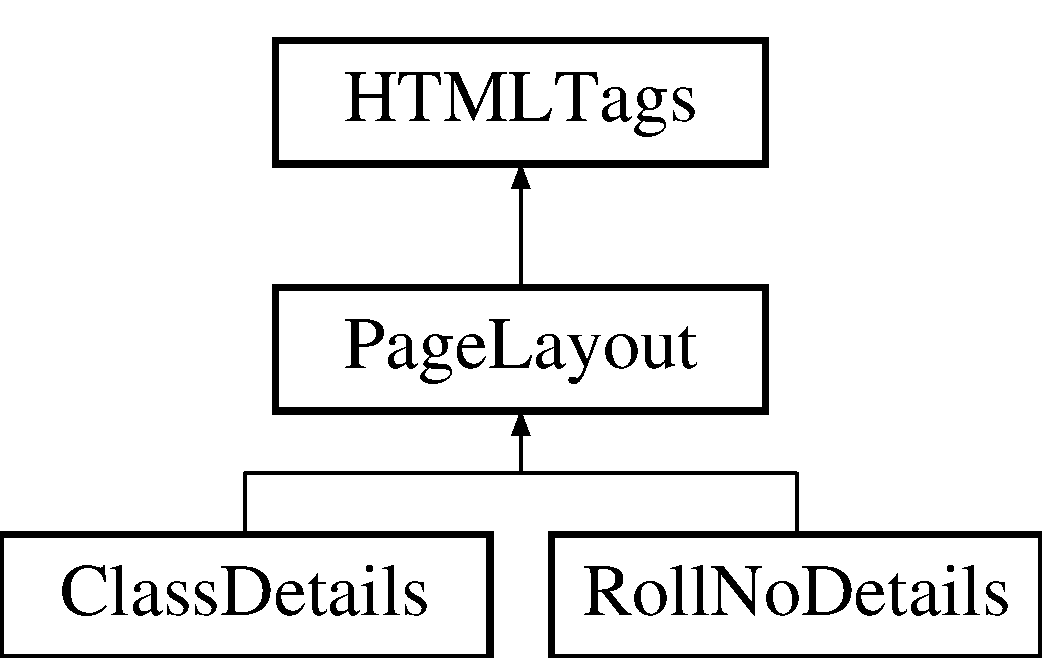
\includegraphics[height=5.000000cm]{classPageLayout}
\end{center}
\end{figure}
\subsection*{Public Member Functions}
\begin{DoxyCompactItemize}
\item 
\hyperlink{classPageLayout_ab3f470f006f9820610d9aaebe5b8427b}{Page\-Layout} ()
\item 
void \hyperlink{classPageLayout_a7726061f0653245f644a05807fa92472}{Header} ()
\item 
void \hyperlink{classPageLayout_a68aa868a8868b12964f161838b5f814c}{Footer} ()
\item 
void \hyperlink{classPageLayout_a49af1dca286bbee9432192a7b3c00332}{Menu} ()
\item 
void \hyperlink{classPageLayout_ae60235c6af48e3ebbc6343d02456da0c}{Logo} (string logo\-Name)
\item 
void \hyperlink{classPageLayout_ae50907d56f0ba7a85f7ccfdeafa45bcc}{Head} (string title\-Name)
\item 
void \hyperlink{classPageLayout_a449b4dde24cf3dc10299dc3c7bfc0e9c}{Set\-Cookies} (string email\-I\-D, string \hyperlink{classPageLayout_ab796c4a12a3f9c089881085e508e2a1c}{session\-I\-D})
\item 
void \hyperlink{classPageLayout_a9884173383d3e9b91e5b4ba6a619caa9}{Context\-Type} ()
\item 
void \hyperlink{classPageLayout_abe2cfa43480c1b48125b3d618cab7831}{Logout\-Link} ()
\item 
void \hyperlink{classPageStructureMaker_aaf78d67380c400cc0057c6519276f721}{Set\-H\-T\-M\-L\-Variables} ()
\item 
void \hyperlink{classPageStructureMaker_ad25d6abc983253567e2370882fc1b407}{H\-T\-M\-L\-Start} ()
\item 
void \hyperlink{classPageStructureMaker_a63b877af1c2c8de8332e3f7eb4c2c2b0}{H\-T\-M\-L\-End} ()
\item 
void \hyperlink{classPageStructureMaker_a14312134cb108f91f2e6d9cbd6916e97}{Head\-Start} ()
\item 
void \hyperlink{classPageStructureMaker_ad64115d592b0989b422a93f85278186e}{Head\-End} ()
\item 
void \hyperlink{classPageStructureMaker_a81e902ddc0c0287df1ba0f614a3774d6}{Title} (string page\-Title)
\item 
void \hyperlink{classPageStructureMaker_aacdb11817f8ab246bc59c552e04e862d}{C\-S\-S} (string href)
\item 
void \hyperlink{classPageStructureMaker_ac221d1169f4dbcef6adb00938919193d}{Javascript} (string src)
\item 
void \hyperlink{classPageStructureMaker_ab7a645675166f34fac99f1ed8feb7c27}{Body\-Start} ()
\item 
void \hyperlink{classPageStructureMaker_ac91e234e2d54dedd9d7e556fabf21d2b}{Body\-End} ()
\item 
void \hyperlink{classPageStructureMaker_a927f92889555dd316c129f706be86a5c}{Div\-Start} (string id, string class\-Name)
\item 
void \hyperlink{classPageStructureMaker_a2913e76bf188ed777dcd33003ef6207d}{Div\-End} ()
\item 
void \hyperlink{classPageStructureMaker_a3f25d5b844a2251883acb80d8fabb77d}{Form\-Start} (string name, string action, string method)
\item 
void \hyperlink{classPageStructureMaker_a65d97f23bb543f3db5201b2009f7f65a}{Form\-End} ()
\item 
void \hyperlink{classPageStructureMaker_a04e68e69005f3933e0f496c3db474daf}{Table\-Start} (string id, string class\-Name)
\item 
void \hyperlink{classPageStructureMaker_a7f8fefbe7a825c1b7761fc8a0f1bb8e4}{Table\-End} ()
\item 
void \hyperlink{classPageStructureMaker_ac24ce26202757aaa30402155daf8a3d0}{List\-Start} (string list\-Type)
\item 
void \hyperlink{classPageStructureMaker_a8578b1555ad2fc92a9efc7dbf7d1fe87}{List\-End} (string list\-Type)
\item 
void \hyperlink{classPageStructureMaker_adf4116e526026edc3c8a3bcf96a7e929}{List\-Item} (string list\-Item)
\item 
void \hyperlink{classPageStructureMaker_a8c0fae5b599182863066de56ae0cea42}{Anchor} (string href, string target)
\item 
void \hyperlink{classPageStructureMaker_a3547027801e298307527f1e934787b13}{Input\-Field} (string type, string name, int name\-No, string value)
\item 
void \hyperlink{classPageStructureMaker_a928ea6f84a8f7833c128034068a4b9a7}{Input\-Field} (string type, string name, string value)
\item 
void \hyperlink{classPageStructureMaker_ae8684bb66ca463e2f92e09c96137f9e3}{Select\-Field\-Start} (string name)
\item 
void \hyperlink{classPageStructureMaker_a81eb3cdbc840a4c8165cef87330ade09}{Select\-Field\-End} ()
\item 
void \hyperlink{classPageStructureMaker_a77856078e74dab25329132ea07466f92}{Select\-Option\-Start} (string value, string selected)
\item 
void \hyperlink{classPageStructureMaker_a7682f479f7f1012d426ec9f9535def60}{Select\-Option\-End} ()
\item 
void \hyperlink{classPageStructureMaker_a419feca1cfdb50e1be757eb1c2707a73}{Button} (string id, string type, string class\-Name, string value)
\end{DoxyCompactItemize}
\subsection*{Protected Attributes}
\begin{DoxyCompactItemize}
\item 
\hypertarget{classPageLayout_a8a3c1ddc422df2556fbc95d0cd575a05}{string {\bfseries project\-Name}}\label{classPageLayout_a8a3c1ddc422df2556fbc95d0cd575a05}

\item 
\hypertarget{classPageLayout_a9abec89a54a6f0dac84114919d2ad117}{ifstream {\bfseries in\-File}}\label{classPageLayout_a9abec89a54a6f0dac84114919d2ad117}

\item 
\hypertarget{classPageLayout_ad52913274f786e82e1e09f5df4bf5347}{ofstream {\bfseries out\-File}}\label{classPageLayout_ad52913274f786e82e1e09f5df4bf5347}

\item 
string \hyperlink{classPageLayout_ab796c4a12a3f9c089881085e508e2a1c}{session\-I\-D}
\item 
string \hyperlink{classPageStructureMaker_af41d4e21b808f5f8dc2c727f775b6fb2}{start\-H1}
\item 
\hypertarget{classPageStructureMaker_a3786a6f477632e4a60205a988d6b599d}{string {\bfseries end\-H1}}\label{classPageStructureMaker_a3786a6f477632e4a60205a988d6b599d}

\item 
\hypertarget{classPageStructureMaker_adb966c147c6328c8e48281c882de776d}{string {\bfseries start\-H3}}\label{classPageStructureMaker_adb966c147c6328c8e48281c882de776d}

\item 
\hypertarget{classPageStructureMaker_a22e6bf3eb787284b745d694613c1d9da}{string {\bfseries end\-H3}}\label{classPageStructureMaker_a22e6bf3eb787284b745d694613c1d9da}

\item 
\hypertarget{classPageStructureMaker_a7e458e675a3adf987a153e08f3795941}{string {\bfseries start\-T\-D}}\label{classPageStructureMaker_a7e458e675a3adf987a153e08f3795941}

\item 
\hypertarget{classPageStructureMaker_ad27f03939a04048a03be0f1bb8edd38a}{string {\bfseries end\-T\-D}}\label{classPageStructureMaker_ad27f03939a04048a03be0f1bb8edd38a}

\item 
\hypertarget{classPageStructureMaker_a4fe234b016efcb9eaa757879b8858190}{string {\bfseries start\-T\-H}}\label{classPageStructureMaker_a4fe234b016efcb9eaa757879b8858190}

\item 
\hypertarget{classPageStructureMaker_aa244b4ef71850dc76fcfb5157bcaf8fc}{string {\bfseries end\-T\-H}}\label{classPageStructureMaker_aa244b4ef71850dc76fcfb5157bcaf8fc}

\item 
\hypertarget{classPageStructureMaker_aa59b4949d26fab5a72710fa9fc3e8ea9}{string {\bfseries start\-T\-R}}\label{classPageStructureMaker_aa59b4949d26fab5a72710fa9fc3e8ea9}

\item 
\hypertarget{classPageStructureMaker_afee49ebdcbc0971142fcf7eae8baa306}{string {\bfseries end\-T\-R}}\label{classPageStructureMaker_afee49ebdcbc0971142fcf7eae8baa306}

\item 
\hypertarget{classPageStructureMaker_aa0f624b485f07f6e19151b1df3dc59a3}{string {\bfseries start\-B}}\label{classPageStructureMaker_aa0f624b485f07f6e19151b1df3dc59a3}

\item 
\hypertarget{classPageStructureMaker_ad46c3195310a1f0226e21d2eb5befb00}{string {\bfseries end\-B}}\label{classPageStructureMaker_ad46c3195310a1f0226e21d2eb5befb00}

\item 
\hypertarget{classPageStructureMaker_a63911cb925ccdc6c879905a677ed8881}{string {\bfseries brk}}\label{classPageStructureMaker_a63911cb925ccdc6c879905a677ed8881}

\end{DoxyCompactItemize}


\subsection{Detailed Description}
-\/-\/-\/-\/-\/-\/-\/-\/-\/-\/-\/-\/-\/-\/-\/-\/-\/-\/-\/-\/-\/-\/-\/-\/-\/-\/-\/-\/-\/-\/-\/-\/-\/-\/-\/-\/-\/-\/-\/-\/-\/-\/-\/-\/-\/-\/-\/-\/-\/-\/-\/-\/-\/-\/-\/-\/-\/-\/-\/-\/-\/-\/-\/-\/-\/-\/-\/ Include required header files ------------------------------------------------------------------ =================================================================== Class\-: \hyperlink{classPageLayout}{Page\-Layout} \-: public \hyperlink{classPageStructureMaker}{Page\-Structure\-Maker} Description\-: For adding header and footer to page =================================================================== 

Definition at line 33 of file pagelayout.\-h.



\subsection{Constructor \& Destructor Documentation}
\hypertarget{classPageLayout_ab3f470f006f9820610d9aaebe5b8427b}{\index{Page\-Layout@{Page\-Layout}!Page\-Layout@{Page\-Layout}}
\index{Page\-Layout@{Page\-Layout}!PageLayout@{Page\-Layout}}
\subsubsection[{Page\-Layout}]{\setlength{\rightskip}{0pt plus 5cm}Page\-Layout\-::\-Page\-Layout (
\begin{DoxyParamCaption}
{}
\end{DoxyParamCaption}
)}}\label{classPageLayout_ab3f470f006f9820610d9aaebe5b8427b}
Constructor

-\/-\/-\/-\/-\/-\/-\/-\/-\/-\/-\/-\/-\/-\/-\/-\/-\/-\/-\/-\/-\/-\/-\/-\/-\/-\/-\/-\/-\/-\/-\/-\/-\/-\/-\/-\/-\/-\/-\/-\/-\/-\/-\/-\/-\/-\/-\/-\/-\/-\/-\/-\/-\/-\/-\/-\/-\/-\/-\/-\/-\/-\/-\/-\/-\/-\/-\/ Include local header file ------------------------------------------------------------------ -\/-\/-\/-\/-\/-\/-\/-\/-\/-\/-\/-\/-\/-\/-\/-\/-\/-\/-\/-\/-\/-\/-\/-\/-\/-\/-\/-\/-\/-\/-\/-\/-\/-\/-\/-\/-\/-\/-\/-\/-\/-\/-\/-\/-\/-\/-\/-\/-\/-\/-\/-\/-\/-\/-\/-\/-\/-\/-\/-\/-\/-\/-\/-\/-\/-\/-\/ Function Definitions of \hyperlink{classPageLayout}{Page\-Layout} Class ------------------------------------------------------------------ -\/-\/-\/-\/-\/-\/-\/-\/-\/-\/-\/-\/-\/-\/-\/-\/-\/-\/-\/-\/-\/-\/-\/-\/-\/-\/-\/-\/-\/-\/-\/-\/-\/-\/-\/-\/-\/-\/-\/-\/-\/-\/-\/-\/-\/-\/-\/-\/-\/-\/-\/-\/-\/-\/-\/-\/-\/-\/-\/-\/-\/-\/-\/-\/-\/-\/-\/-\/ Class\-: \hyperlink{classPageLayout}{Page\-Layout} Method\-: \hyperlink{classPageLayout}{Page\-Layout} \-:\-: \hyperlink{classPageLayout_ab3f470f006f9820610d9aaebe5b8427b}{Page\-Layout()} Description\-: Constructor -\/-\/-\/-\/-\/-\/-\/-\/-\/-\/-\/-\/-\/-\/-\/-\/-\/-\/-\/-\/-\/-\/-\/-\/-\/-\/-\/-\/-\/-\/-\/-\/-\/-\/-\/-\/-\/-\/-\/-\/-\/-\/-\/-\/-\/-\/-\/-\/-\/-\/-\/-\/-\/-\/-\/-\/-\/-\/-\/-\/-\/-\/-\/-\/-\/-\/-\/-\/ 

Definition at line 38 of file pagelayout.\-cc.



\subsection{Member Function Documentation}
\hypertarget{classPageStructureMaker_a8c0fae5b599182863066de56ae0cea42}{\index{Page\-Layout@{Page\-Layout}!Anchor@{Anchor}}
\index{Anchor@{Anchor}!PageLayout@{Page\-Layout}}
\subsubsection[{Anchor}]{\setlength{\rightskip}{0pt plus 5cm}void Page\-Structure\-Maker\-::\-Anchor (
\begin{DoxyParamCaption}
\item[{string}]{href, }
\item[{string}]{target}
\end{DoxyParamCaption}
)\hspace{0.3cm}{\ttfamily [inherited]}}}\label{classPageStructureMaker_a8c0fae5b599182863066de56ae0cea42}
Anchor Tag

--------------------------------------------------------------------\par
 Class\-: \hyperlink{classPageStructureMaker}{Page\-Structure\-Maker} \par
 Method\-: \hyperlink{classPageStructureMaker}{Page\-Structure\-Maker} \-:\-: Anchor(string href) \par
 Description\-: Anchor Tag \par
 -\/-\/-\/-\/-\/-\/-\/-\/-\/-\/-\/-\/-\/-\/-\/-\/-\/-\/-\/-\/-\/-\/-\/-\/-\/-\/-\/-\/-\/-\/-\/-\/-\/-\/-\/-\/-\/-\/-\/-\/-\/-\/-\/-\/-\/-\/-\/-\/-\/-\/-\/-\/-\/-\/-\/-\/-\/-\/-\/-\/-\/-\/-\/-\/-\/-\/-\/-\/ 

Definition at line 318 of file pagestructure.\-cc.

\hypertarget{classPageStructureMaker_ac91e234e2d54dedd9d7e556fabf21d2b}{\index{Page\-Layout@{Page\-Layout}!Body\-End@{Body\-End}}
\index{Body\-End@{Body\-End}!PageLayout@{Page\-Layout}}
\subsubsection[{Body\-End}]{\setlength{\rightskip}{0pt plus 5cm}void Page\-Structure\-Maker\-::\-Body\-End (
\begin{DoxyParamCaption}
{}
\end{DoxyParamCaption}
)\hspace{0.3cm}{\ttfamily [inherited]}}}\label{classPageStructureMaker_ac91e234e2d54dedd9d7e556fabf21d2b}
Display $<$/\-B\-O\-D\-Y$>$

-\/-\/-\/-\/-\/-\/-\/-\/-\/-\/-\/-\/-\/-\/-\/-\/-\/-\/-\/-\/-\/-\/-\/-\/-\/-\/-\/-\/-\/-\/-\/-\/-\/-\/-\/-\/-\/-\/-\/-\/-\/-\/-\/-\/-\/-\/-\/-\/-\/-\/-\/-\/-\/-\/-\/-\/-\/-\/-\/-\/-\/-\/-\/-\/-\/-\/-\/-\/ Class\-: \hyperlink{classPageStructureMaker}{Page\-Structure\-Maker} Method\-: \hyperlink{classPageStructureMaker}{Page\-Structure\-Maker} \-:\-: \hyperlink{classPageStructureMaker_ac91e234e2d54dedd9d7e556fabf21d2b}{Body\-End()} Description\-: Display $<$/\-B\-O\-D\-Y$>$ -\/-\/-\/-\/-\/-\/-\/-\/-\/-\/-\/-\/-\/-\/-\/-\/-\/-\/-\/-\/-\/-\/-\/-\/-\/-\/-\/-\/-\/-\/-\/-\/-\/-\/-\/-\/-\/-\/-\/-\/-\/-\/-\/-\/-\/-\/-\/-\/-\/-\/-\/-\/-\/-\/-\/-\/-\/-\/-\/-\/-\/-\/-\/-\/-\/-\/-\/-\/ 

Definition at line 180 of file pagestructure.\-cc.

\hypertarget{classPageStructureMaker_ab7a645675166f34fac99f1ed8feb7c27}{\index{Page\-Layout@{Page\-Layout}!Body\-Start@{Body\-Start}}
\index{Body\-Start@{Body\-Start}!PageLayout@{Page\-Layout}}
\subsubsection[{Body\-Start}]{\setlength{\rightskip}{0pt plus 5cm}void Page\-Structure\-Maker\-::\-Body\-Start (
\begin{DoxyParamCaption}
{}
\end{DoxyParamCaption}
)\hspace{0.3cm}{\ttfamily [inherited]}}}\label{classPageStructureMaker_ab7a645675166f34fac99f1ed8feb7c27}
Display $<$\-B\-O\-D\-Y$>$

-\/-\/-\/-\/-\/-\/-\/-\/-\/-\/-\/-\/-\/-\/-\/-\/-\/-\/-\/-\/-\/-\/-\/-\/-\/-\/-\/-\/-\/-\/-\/-\/-\/-\/-\/-\/-\/-\/-\/-\/-\/-\/-\/-\/-\/-\/-\/-\/-\/-\/-\/-\/-\/-\/-\/-\/-\/-\/-\/-\/-\/-\/-\/-\/-\/-\/-\/-\/ Class\-: \hyperlink{classPageStructureMaker}{Page\-Structure\-Maker} Method\-: \hyperlink{classPageStructureMaker}{Page\-Structure\-Maker} \-:\-: \hyperlink{classPageStructureMaker_ab7a645675166f34fac99f1ed8feb7c27}{Body\-Start()} Description\-: Display $<$B\-O\-D\-Y$>$ -\/-\/-\/-\/-\/-\/-\/-\/-\/-\/-\/-\/-\/-\/-\/-\/-\/-\/-\/-\/-\/-\/-\/-\/-\/-\/-\/-\/-\/-\/-\/-\/-\/-\/-\/-\/-\/-\/-\/-\/-\/-\/-\/-\/-\/-\/-\/-\/-\/-\/-\/-\/-\/-\/-\/-\/-\/-\/-\/-\/-\/-\/-\/-\/-\/-\/-\/-\/ 

Definition at line 166 of file pagestructure.\-cc.

\hypertarget{classPageStructureMaker_a419feca1cfdb50e1be757eb1c2707a73}{\index{Page\-Layout@{Page\-Layout}!Button@{Button}}
\index{Button@{Button}!PageLayout@{Page\-Layout}}
\subsubsection[{Button}]{\setlength{\rightskip}{0pt plus 5cm}void Page\-Structure\-Maker\-::\-Button (
\begin{DoxyParamCaption}
\item[{string}]{id, }
\item[{string}]{type, }
\item[{string}]{class\-Name, }
\item[{string}]{value}
\end{DoxyParamCaption}
)\hspace{0.3cm}{\ttfamily [inherited]}}}\label{classPageStructureMaker_a419feca1cfdb50e1be757eb1c2707a73}
Button

-\/-\/-\/-\/-\/-\/-\/-\/-\/-\/-\/-\/-\/-\/-\/-\/-\/-\/-\/-\/-\/-\/-\/-\/-\/-\/-\/-\/-\/-\/-\/-\/-\/-\/-\/-\/-\/-\/-\/-\/-\/-\/-\/-\/-\/-\/-\/-\/-\/-\/-\/-\/-\/-\/-\/-\/-\/-\/-\/-\/-\/-\/-\/-\/-\/-\/-\/-\/ Class\-: \hyperlink{classPageStructureMaker}{Page\-Structure\-Maker} Method\-: \hyperlink{classPageStructureMaker}{Page\-Structure\-Maker} \-:\-: Button(string id, string type, string class\-Name, string value) Description\-: Create button(next, submit, etc) -\/-\/-\/-\/-\/-\/-\/-\/-\/-\/-\/-\/-\/-\/-\/-\/-\/-\/-\/-\/-\/-\/-\/-\/-\/-\/-\/-\/-\/-\/-\/-\/-\/-\/-\/-\/-\/-\/-\/-\/-\/-\/-\/-\/-\/-\/-\/-\/-\/-\/-\/-\/-\/-\/-\/-\/-\/-\/-\/-\/-\/-\/-\/-\/-\/-\/-\/-\/ 

Definition at line 436 of file pagestructure.\-cc.

\hypertarget{classPageLayout_a9884173383d3e9b91e5b4ba6a619caa9}{\index{Page\-Layout@{Page\-Layout}!Context\-Type@{Context\-Type}}
\index{Context\-Type@{Context\-Type}!PageLayout@{Page\-Layout}}
\subsubsection[{Context\-Type}]{\setlength{\rightskip}{0pt plus 5cm}void Page\-Layout\-::\-Context\-Type (
\begin{DoxyParamCaption}
{}
\end{DoxyParamCaption}
)}}\label{classPageLayout_a9884173383d3e9b91e5b4ba6a619caa9}
Context-\/\-Type header

--------------------------------------------------------------------\par
 Class\-: \hyperlink{classPageLayout}{Page\-Layout} \par
 Method\-: \hyperlink{classPageLayout}{Page\-Layout} \-:\-: Context\-Type \par
 Description\-: Setting content-\/type header \par
 -\/-\/-\/-\/-\/-\/-\/-\/-\/-\/-\/-\/-\/-\/-\/-\/-\/-\/-\/-\/-\/-\/-\/-\/-\/-\/-\/-\/-\/-\/-\/-\/-\/-\/-\/-\/-\/-\/-\/-\/-\/-\/-\/-\/-\/-\/-\/-\/-\/-\/-\/-\/-\/-\/-\/-\/-\/-\/-\/-\/-\/-\/-\/-\/-\/-\/-\/-\/ 

Definition at line 162 of file pagelayout.\-cc.

\hypertarget{classPageStructureMaker_aacdb11817f8ab246bc59c552e04e862d}{\index{Page\-Layout@{Page\-Layout}!C\-S\-S@{C\-S\-S}}
\index{C\-S\-S@{C\-S\-S}!PageLayout@{Page\-Layout}}
\subsubsection[{C\-S\-S}]{\setlength{\rightskip}{0pt plus 5cm}void Page\-Structure\-Maker\-::\-C\-S\-S (
\begin{DoxyParamCaption}
\item[{string}]{href}
\end{DoxyParamCaption}
)\hspace{0.3cm}{\ttfamily [inherited]}}}\label{classPageStructureMaker_aacdb11817f8ab246bc59c552e04e862d}
Add External C\-S\-S

-\/-\/-\/-\/-\/-\/-\/-\/-\/-\/-\/-\/-\/-\/-\/-\/-\/-\/-\/-\/-\/-\/-\/-\/-\/-\/-\/-\/-\/-\/-\/-\/-\/-\/-\/-\/-\/-\/-\/-\/-\/-\/-\/-\/-\/-\/-\/-\/-\/-\/-\/-\/-\/-\/-\/-\/-\/-\/-\/-\/-\/-\/-\/-\/-\/-\/-\/-\/ Class\-: \hyperlink{classPageStructureMaker}{Page\-Structure\-Maker} Method\-: \hyperlink{classPageStructureMaker}{Page\-Structure\-Maker} \-:\-: \hyperlink{classPageStructureMaker_aacdb11817f8ab246bc59c552e04e862d}{C\-S\-S(string href)} Description\-: Add External C\-S\-S file -\/-\/-\/-\/-\/-\/-\/-\/-\/-\/-\/-\/-\/-\/-\/-\/-\/-\/-\/-\/-\/-\/-\/-\/-\/-\/-\/-\/-\/-\/-\/-\/-\/-\/-\/-\/-\/-\/-\/-\/-\/-\/-\/-\/-\/-\/-\/-\/-\/-\/-\/-\/-\/-\/-\/-\/-\/-\/-\/-\/-\/-\/-\/-\/-\/-\/-\/-\/ 

Definition at line 138 of file pagestructure.\-cc.

\hypertarget{classPageStructureMaker_a2913e76bf188ed777dcd33003ef6207d}{\index{Page\-Layout@{Page\-Layout}!Div\-End@{Div\-End}}
\index{Div\-End@{Div\-End}!PageLayout@{Page\-Layout}}
\subsubsection[{Div\-End}]{\setlength{\rightskip}{0pt plus 5cm}void Page\-Structure\-Maker\-::\-Div\-End (
\begin{DoxyParamCaption}
{}
\end{DoxyParamCaption}
)\hspace{0.3cm}{\ttfamily [inherited]}}}\label{classPageStructureMaker_a2913e76bf188ed777dcd33003ef6207d}
End div section

-\/-\/-\/-\/-\/-\/-\/-\/-\/-\/-\/-\/-\/-\/-\/-\/-\/-\/-\/-\/-\/-\/-\/-\/-\/-\/-\/-\/-\/-\/-\/-\/-\/-\/-\/-\/-\/-\/-\/-\/-\/-\/-\/-\/-\/-\/-\/-\/-\/-\/-\/-\/-\/-\/-\/-\/-\/-\/-\/-\/-\/-\/-\/-\/-\/-\/-\/-\/ Class\-: \hyperlink{classPageStructureMaker}{Page\-Structure\-Maker} Method\-: \hyperlink{classPageStructureMaker}{Page\-Structure\-Maker} \-:\-: \hyperlink{classPageStructureMaker_a2913e76bf188ed777dcd33003ef6207d}{Div\-End()} Description\-: Close Div Section -\/-\/-\/-\/-\/-\/-\/-\/-\/-\/-\/-\/-\/-\/-\/-\/-\/-\/-\/-\/-\/-\/-\/-\/-\/-\/-\/-\/-\/-\/-\/-\/-\/-\/-\/-\/-\/-\/-\/-\/-\/-\/-\/-\/-\/-\/-\/-\/-\/-\/-\/-\/-\/-\/-\/-\/-\/-\/-\/-\/-\/-\/-\/-\/-\/-\/-\/-\/ 

Definition at line 209 of file pagestructure.\-cc.

\hypertarget{classPageStructureMaker_a927f92889555dd316c129f706be86a5c}{\index{Page\-Layout@{Page\-Layout}!Div\-Start@{Div\-Start}}
\index{Div\-Start@{Div\-Start}!PageLayout@{Page\-Layout}}
\subsubsection[{Div\-Start}]{\setlength{\rightskip}{0pt plus 5cm}void Page\-Structure\-Maker\-::\-Div\-Start (
\begin{DoxyParamCaption}
\item[{string}]{id, }
\item[{string}]{class\-Name}
\end{DoxyParamCaption}
)\hspace{0.3cm}{\ttfamily [inherited]}}}\label{classPageStructureMaker_a927f92889555dd316c129f706be86a5c}
Start Div Section

-\/-\/-\/-\/-\/-\/-\/-\/-\/-\/-\/-\/-\/-\/-\/-\/-\/-\/-\/-\/-\/-\/-\/-\/-\/-\/-\/-\/-\/-\/-\/-\/-\/-\/-\/-\/-\/-\/-\/-\/-\/-\/-\/-\/-\/-\/-\/-\/-\/-\/-\/-\/-\/-\/-\/-\/-\/-\/-\/-\/-\/-\/-\/-\/-\/-\/-\/-\/ Class\-: \hyperlink{classPageStructureMaker}{Page\-Structure\-Maker} Method\-: \hyperlink{classPageStructureMaker}{Page\-Structure\-Maker} \-:\-: Div\-Start(string id, string class\-Name) Description\-: Start Div Section with id and class\-Name(for C\-S\-S) -\/-\/-\/-\/-\/-\/-\/-\/-\/-\/-\/-\/-\/-\/-\/-\/-\/-\/-\/-\/-\/-\/-\/-\/-\/-\/-\/-\/-\/-\/-\/-\/-\/-\/-\/-\/-\/-\/-\/-\/-\/-\/-\/-\/-\/-\/-\/-\/-\/-\/-\/-\/-\/-\/-\/-\/-\/-\/-\/-\/-\/-\/-\/-\/-\/-\/-\/-\/ 

Definition at line 195 of file pagestructure.\-cc.

\hypertarget{classPageLayout_a68aa868a8868b12964f161838b5f814c}{\index{Page\-Layout@{Page\-Layout}!Footer@{Footer}}
\index{Footer@{Footer}!PageLayout@{Page\-Layout}}
\subsubsection[{Footer}]{\setlength{\rightskip}{0pt plus 5cm}void Page\-Layout\-::\-Footer (
\begin{DoxyParamCaption}
{}
\end{DoxyParamCaption}
)}}\label{classPageLayout_a68aa868a8868b12964f161838b5f814c}
Footer Section of Page

-\/-\/-\/-\/-\/-\/-\/-\/-\/-\/-\/-\/-\/-\/-\/-\/-\/-\/-\/-\/-\/-\/-\/-\/-\/-\/-\/-\/-\/-\/-\/-\/-\/-\/-\/-\/-\/-\/-\/-\/-\/-\/-\/-\/-\/-\/-\/-\/-\/-\/-\/-\/-\/-\/-\/-\/-\/-\/-\/-\/-\/-\/-\/-\/-\/-\/-\/-\/ Class\-: \hyperlink{classPageLayout}{Page\-Layout} Method\-: \hyperlink{classPageLayout}{Page\-Layout} \-:\-: \hyperlink{classPageLayout_a68aa868a8868b12964f161838b5f814c}{Footer()} Description\-: Footer of pages -\/-\/-\/-\/-\/-\/-\/-\/-\/-\/-\/-\/-\/-\/-\/-\/-\/-\/-\/-\/-\/-\/-\/-\/-\/-\/-\/-\/-\/-\/-\/-\/-\/-\/-\/-\/-\/-\/-\/-\/-\/-\/-\/-\/-\/-\/-\/-\/-\/-\/-\/-\/-\/-\/-\/-\/-\/-\/-\/-\/-\/-\/-\/-\/-\/-\/-\/-\/ 

Reimplemented in \hyperlink{classInputDetail_acbc05b1bc6a371cf0a52222cc95e467d}{Input\-Detail}.



Definition at line 190 of file pagelayout.\-cc.

\hypertarget{classPageStructureMaker_a65d97f23bb543f3db5201b2009f7f65a}{\index{Page\-Layout@{Page\-Layout}!Form\-End@{Form\-End}}
\index{Form\-End@{Form\-End}!PageLayout@{Page\-Layout}}
\subsubsection[{Form\-End}]{\setlength{\rightskip}{0pt plus 5cm}void Page\-Structure\-Maker\-::\-Form\-End (
\begin{DoxyParamCaption}
{}
\end{DoxyParamCaption}
)\hspace{0.3cm}{\ttfamily [inherited]}}}\label{classPageStructureMaker_a65d97f23bb543f3db5201b2009f7f65a}
End Form

-\/-\/-\/-\/-\/-\/-\/-\/-\/-\/-\/-\/-\/-\/-\/-\/-\/-\/-\/-\/-\/-\/-\/-\/-\/-\/-\/-\/-\/-\/-\/-\/-\/-\/-\/-\/-\/-\/-\/-\/-\/-\/-\/-\/-\/-\/-\/-\/-\/-\/-\/-\/-\/-\/-\/-\/-\/-\/-\/-\/-\/-\/-\/-\/-\/-\/-\/-\/ Class\-: \hyperlink{classPageStructureMaker}{Page\-Structure\-Maker} Method\-: \hyperlink{classPageStructureMaker}{Page\-Structure\-Maker} \-:\-: \hyperlink{classPageStructureMaker_a65d97f23bb543f3db5201b2009f7f65a}{Form\-End()} Description\-: Close Form -\/-\/-\/-\/-\/-\/-\/-\/-\/-\/-\/-\/-\/-\/-\/-\/-\/-\/-\/-\/-\/-\/-\/-\/-\/-\/-\/-\/-\/-\/-\/-\/-\/-\/-\/-\/-\/-\/-\/-\/-\/-\/-\/-\/-\/-\/-\/-\/-\/-\/-\/-\/-\/-\/-\/-\/-\/-\/-\/-\/-\/-\/-\/-\/-\/-\/-\/-\/ 

Definition at line 238 of file pagestructure.\-cc.

\hypertarget{classPageStructureMaker_a3f25d5b844a2251883acb80d8fabb77d}{\index{Page\-Layout@{Page\-Layout}!Form\-Start@{Form\-Start}}
\index{Form\-Start@{Form\-Start}!PageLayout@{Page\-Layout}}
\subsubsection[{Form\-Start}]{\setlength{\rightskip}{0pt plus 5cm}void Page\-Structure\-Maker\-::\-Form\-Start (
\begin{DoxyParamCaption}
\item[{string}]{name, }
\item[{string}]{action, }
\item[{string}]{method}
\end{DoxyParamCaption}
)\hspace{0.3cm}{\ttfamily [inherited]}}}\label{classPageStructureMaker_a3f25d5b844a2251883acb80d8fabb77d}
Start Form

-\/-\/-\/-\/-\/-\/-\/-\/-\/-\/-\/-\/-\/-\/-\/-\/-\/-\/-\/-\/-\/-\/-\/-\/-\/-\/-\/-\/-\/-\/-\/-\/-\/-\/-\/-\/-\/-\/-\/-\/-\/-\/-\/-\/-\/-\/-\/-\/-\/-\/-\/-\/-\/-\/-\/-\/-\/-\/-\/-\/-\/-\/-\/-\/-\/-\/-\/-\/ Class\-: \hyperlink{classPageStructureMaker}{Page\-Structure\-Maker} Method\-: \hyperlink{classPageStructureMaker}{Page\-Structure\-Maker} \-:\-: Form\-Start(string name, string action, string method) Description\-: Start Form with name, action and method(G\-E\-T/\-P\-O\-S\-T) -\/-\/-\/-\/-\/-\/-\/-\/-\/-\/-\/-\/-\/-\/-\/-\/-\/-\/-\/-\/-\/-\/-\/-\/-\/-\/-\/-\/-\/-\/-\/-\/-\/-\/-\/-\/-\/-\/-\/-\/-\/-\/-\/-\/-\/-\/-\/-\/-\/-\/-\/-\/-\/-\/-\/-\/-\/-\/-\/-\/-\/-\/-\/-\/-\/-\/-\/-\/ 

Definition at line 223 of file pagestructure.\-cc.

\hypertarget{classPageLayout_ae50907d56f0ba7a85f7ccfdeafa45bcc}{\index{Page\-Layout@{Page\-Layout}!Head@{Head}}
\index{Head@{Head}!PageLayout@{Page\-Layout}}
\subsubsection[{Head}]{\setlength{\rightskip}{0pt plus 5cm}void Page\-Layout\-::\-Head (
\begin{DoxyParamCaption}
\item[{string}]{title\-Name}
\end{DoxyParamCaption}
)}}\label{classPageLayout_ae50907d56f0ba7a85f7ccfdeafa45bcc}
Head Section of Page

-\/-\/-\/-\/-\/-\/-\/-\/-\/-\/-\/-\/-\/-\/-\/-\/-\/-\/-\/-\/-\/-\/-\/-\/-\/-\/-\/-\/-\/-\/-\/-\/-\/-\/-\/-\/-\/-\/-\/-\/-\/-\/-\/-\/-\/-\/-\/-\/-\/-\/-\/-\/-\/-\/-\/-\/-\/-\/-\/-\/-\/-\/-\/-\/-\/-\/-\/-\/ Class\-: \hyperlink{classPageLayout}{Page\-Layout} Method\-: \hyperlink{classPageLayout}{Page\-Layout} \-:\-: \hyperlink{classPageLayout_ae50907d56f0ba7a85f7ccfdeafa45bcc}{Head(string title\-Name)} Description\-: Head Section of page, titla\-Name pass to Title function. -\/-\/-\/-\/-\/-\/-\/-\/-\/-\/-\/-\/-\/-\/-\/-\/-\/-\/-\/-\/-\/-\/-\/-\/-\/-\/-\/-\/-\/-\/-\/-\/-\/-\/-\/-\/-\/-\/-\/-\/-\/-\/-\/-\/-\/-\/-\/-\/-\/-\/-\/-\/-\/-\/-\/-\/-\/-\/-\/-\/-\/-\/-\/-\/-\/-\/-\/-\/ 

Definition at line 106 of file pagelayout.\-cc.

\hypertarget{classPageStructureMaker_ad64115d592b0989b422a93f85278186e}{\index{Page\-Layout@{Page\-Layout}!Head\-End@{Head\-End}}
\index{Head\-End@{Head\-End}!PageLayout@{Page\-Layout}}
\subsubsection[{Head\-End}]{\setlength{\rightskip}{0pt plus 5cm}void Page\-Structure\-Maker\-::\-Head\-End (
\begin{DoxyParamCaption}
{}
\end{DoxyParamCaption}
)\hspace{0.3cm}{\ttfamily [inherited]}}}\label{classPageStructureMaker_ad64115d592b0989b422a93f85278186e}
Display $<$/\-H\-E\-A\-D$>$

-\/-\/-\/-\/-\/-\/-\/-\/-\/-\/-\/-\/-\/-\/-\/-\/-\/-\/-\/-\/-\/-\/-\/-\/-\/-\/-\/-\/-\/-\/-\/-\/-\/-\/-\/-\/-\/-\/-\/-\/-\/-\/-\/-\/-\/-\/-\/-\/-\/-\/-\/-\/-\/-\/-\/-\/-\/-\/-\/-\/-\/-\/-\/-\/-\/-\/-\/-\/ Class\-: \hyperlink{classPageStructureMaker}{Page\-Structure\-Maker} Method\-: \hyperlink{classPageStructureMaker}{Page\-Structure\-Maker} \-:\-: \hyperlink{classPageStructureMaker_ad64115d592b0989b422a93f85278186e}{Head\-End()} Description\-: Display $<$/\-H\-E\-A\-D$>$ -\/-\/-\/-\/-\/-\/-\/-\/-\/-\/-\/-\/-\/-\/-\/-\/-\/-\/-\/-\/-\/-\/-\/-\/-\/-\/-\/-\/-\/-\/-\/-\/-\/-\/-\/-\/-\/-\/-\/-\/-\/-\/-\/-\/-\/-\/-\/-\/-\/-\/-\/-\/-\/-\/-\/-\/-\/-\/-\/-\/-\/-\/-\/-\/-\/-\/-\/-\/ 

Definition at line 112 of file pagestructure.\-cc.

\hypertarget{classPageLayout_a7726061f0653245f644a05807fa92472}{\index{Page\-Layout@{Page\-Layout}!Header@{Header}}
\index{Header@{Header}!PageLayout@{Page\-Layout}}
\subsubsection[{Header}]{\setlength{\rightskip}{0pt plus 5cm}void Page\-Layout\-::\-Header (
\begin{DoxyParamCaption}
{}
\end{DoxyParamCaption}
)}}\label{classPageLayout_a7726061f0653245f644a05807fa92472}
Header Section of Page

-\/-\/-\/-\/-\/-\/-\/-\/-\/-\/-\/-\/-\/-\/-\/-\/-\/-\/-\/-\/-\/-\/-\/-\/-\/-\/-\/-\/-\/-\/-\/-\/-\/-\/-\/-\/-\/-\/-\/-\/-\/-\/-\/-\/-\/-\/-\/-\/-\/-\/-\/-\/-\/-\/-\/-\/-\/-\/-\/-\/-\/-\/-\/-\/-\/-\/-\/-\/ Class\-: \hyperlink{classPageLayout}{Page\-Layout} Method\-: \hyperlink{classPageLayout}{Page\-Layout} \-:\-: \hyperlink{classPageLayout_a7726061f0653245f644a05807fa92472}{Header()} Description\-: Call Menu Function -\/-\/-\/-\/-\/-\/-\/-\/-\/-\/-\/-\/-\/-\/-\/-\/-\/-\/-\/-\/-\/-\/-\/-\/-\/-\/-\/-\/-\/-\/-\/-\/-\/-\/-\/-\/-\/-\/-\/-\/-\/-\/-\/-\/-\/-\/-\/-\/-\/-\/-\/-\/-\/-\/-\/-\/-\/-\/-\/-\/-\/-\/-\/-\/-\/-\/-\/-\/ 

Definition at line 89 of file pagelayout.\-cc.

\hypertarget{classPageStructureMaker_a14312134cb108f91f2e6d9cbd6916e97}{\index{Page\-Layout@{Page\-Layout}!Head\-Start@{Head\-Start}}
\index{Head\-Start@{Head\-Start}!PageLayout@{Page\-Layout}}
\subsubsection[{Head\-Start}]{\setlength{\rightskip}{0pt plus 5cm}void Page\-Structure\-Maker\-::\-Head\-Start (
\begin{DoxyParamCaption}
{}
\end{DoxyParamCaption}
)\hspace{0.3cm}{\ttfamily [inherited]}}}\label{classPageStructureMaker_a14312134cb108f91f2e6d9cbd6916e97}
Display $<$\-H\-E\-A\-D$>$

-\/-\/-\/-\/-\/-\/-\/-\/-\/-\/-\/-\/-\/-\/-\/-\/-\/-\/-\/-\/-\/-\/-\/-\/-\/-\/-\/-\/-\/-\/-\/-\/-\/-\/-\/-\/-\/-\/-\/-\/-\/-\/-\/-\/-\/-\/-\/-\/-\/-\/-\/-\/-\/-\/-\/-\/-\/-\/-\/-\/-\/-\/-\/-\/-\/-\/-\/-\/ Class\-: \hyperlink{classPageStructureMaker}{Page\-Structure\-Maker} Method\-: \hyperlink{classPageStructureMaker}{Page\-Structure\-Maker} \-:\-: \hyperlink{classPageStructureMaker_a14312134cb108f91f2e6d9cbd6916e97}{Head\-Start()} Description\-: Display $<$H\-E\-A\-D$>$ -\/-\/-\/-\/-\/-\/-\/-\/-\/-\/-\/-\/-\/-\/-\/-\/-\/-\/-\/-\/-\/-\/-\/-\/-\/-\/-\/-\/-\/-\/-\/-\/-\/-\/-\/-\/-\/-\/-\/-\/-\/-\/-\/-\/-\/-\/-\/-\/-\/-\/-\/-\/-\/-\/-\/-\/-\/-\/-\/-\/-\/-\/-\/-\/-\/-\/-\/-\/ 

Definition at line 99 of file pagestructure.\-cc.

\hypertarget{classPageStructureMaker_a63b877af1c2c8de8332e3f7eb4c2c2b0}{\index{Page\-Layout@{Page\-Layout}!H\-T\-M\-L\-End@{H\-T\-M\-L\-End}}
\index{H\-T\-M\-L\-End@{H\-T\-M\-L\-End}!PageLayout@{Page\-Layout}}
\subsubsection[{H\-T\-M\-L\-End}]{\setlength{\rightskip}{0pt plus 5cm}void Page\-Structure\-Maker\-::\-H\-T\-M\-L\-End (
\begin{DoxyParamCaption}
{}
\end{DoxyParamCaption}
)\hspace{0.3cm}{\ttfamily [inherited]}}}\label{classPageStructureMaker_a63b877af1c2c8de8332e3f7eb4c2c2b0}
Display $<$/\-H\-T\-M\-L$>$

-\/-\/-\/-\/-\/-\/-\/-\/-\/-\/-\/-\/-\/-\/-\/-\/-\/-\/-\/-\/-\/-\/-\/-\/-\/-\/-\/-\/-\/-\/-\/-\/-\/-\/-\/-\/-\/-\/-\/-\/-\/-\/-\/-\/-\/-\/-\/-\/-\/-\/-\/-\/-\/-\/-\/-\/-\/-\/-\/-\/-\/-\/-\/-\/-\/-\/-\/-\/ Class\-: \hyperlink{classPageStructureMaker}{Page\-Structure\-Maker} Method\-: \hyperlink{classPageStructureMaker}{Page\-Structure\-Maker} \-:\-: \hyperlink{classPageStructureMaker_a63b877af1c2c8de8332e3f7eb4c2c2b0}{H\-T\-M\-L\-End()} Description\-: Display $<$/\-H\-T\-M\-L$>$ -\/-\/-\/-\/-\/-\/-\/-\/-\/-\/-\/-\/-\/-\/-\/-\/-\/-\/-\/-\/-\/-\/-\/-\/-\/-\/-\/-\/-\/-\/-\/-\/-\/-\/-\/-\/-\/-\/-\/-\/-\/-\/-\/-\/-\/-\/-\/-\/-\/-\/-\/-\/-\/-\/-\/-\/-\/-\/-\/-\/-\/-\/-\/-\/-\/-\/-\/-\/ 

Definition at line 86 of file pagestructure.\-cc.

\hypertarget{classPageStructureMaker_ad25d6abc983253567e2370882fc1b407}{\index{Page\-Layout@{Page\-Layout}!H\-T\-M\-L\-Start@{H\-T\-M\-L\-Start}}
\index{H\-T\-M\-L\-Start@{H\-T\-M\-L\-Start}!PageLayout@{Page\-Layout}}
\subsubsection[{H\-T\-M\-L\-Start}]{\setlength{\rightskip}{0pt plus 5cm}void Page\-Structure\-Maker\-::\-H\-T\-M\-L\-Start (
\begin{DoxyParamCaption}
{}
\end{DoxyParamCaption}
)\hspace{0.3cm}{\ttfamily [inherited]}}}\label{classPageStructureMaker_ad25d6abc983253567e2370882fc1b407}
Display $<$\-H\-T\-M\-L$>$

-\/-\/-\/-\/-\/-\/-\/-\/-\/-\/-\/-\/-\/-\/-\/-\/-\/-\/-\/-\/-\/-\/-\/-\/-\/-\/-\/-\/-\/-\/-\/-\/-\/-\/-\/-\/-\/-\/-\/-\/-\/-\/-\/-\/-\/-\/-\/-\/-\/-\/-\/-\/-\/-\/-\/-\/-\/-\/-\/-\/-\/-\/-\/-\/-\/-\/-\/-\/ Class\-: \hyperlink{classPageStructureMaker}{Page\-Structure\-Maker} Method\-: \hyperlink{classPageStructureMaker}{Page\-Structure\-Maker} \-:\-: \hyperlink{classPageStructureMaker_ad25d6abc983253567e2370882fc1b407}{H\-T\-M\-L\-Start()} Description\-: Display $<$H\-T\-M\-L$>$ Tag -\/-\/-\/-\/-\/-\/-\/-\/-\/-\/-\/-\/-\/-\/-\/-\/-\/-\/-\/-\/-\/-\/-\/-\/-\/-\/-\/-\/-\/-\/-\/-\/-\/-\/-\/-\/-\/-\/-\/-\/-\/-\/-\/-\/-\/-\/-\/-\/-\/-\/-\/-\/-\/-\/-\/-\/-\/-\/-\/-\/-\/-\/-\/-\/-\/-\/-\/-\/ 

Definition at line 73 of file pagestructure.\-cc.

\hypertarget{classPageStructureMaker_a3547027801e298307527f1e934787b13}{\index{Page\-Layout@{Page\-Layout}!Input\-Field@{Input\-Field}}
\index{Input\-Field@{Input\-Field}!PageLayout@{Page\-Layout}}
\subsubsection[{Input\-Field}]{\setlength{\rightskip}{0pt plus 5cm}void Page\-Structure\-Maker\-::\-Input\-Field (
\begin{DoxyParamCaption}
\item[{string}]{type, }
\item[{string}]{name, }
\item[{int}]{name\-No, }
\item[{string}]{value}
\end{DoxyParamCaption}
)\hspace{0.3cm}{\ttfamily [inherited]}}}\label{classPageStructureMaker_a3547027801e298307527f1e934787b13}
Input Field with 4 arguments

-\/-\/-\/-\/-\/-\/-\/-\/-\/-\/-\/-\/-\/-\/-\/-\/-\/-\/-\/-\/-\/-\/-\/-\/-\/-\/-\/-\/-\/-\/-\/-\/-\/-\/-\/-\/-\/-\/-\/-\/-\/-\/-\/-\/-\/-\/-\/-\/-\/-\/-\/-\/-\/-\/-\/-\/-\/-\/-\/-\/-\/-\/-\/-\/-\/-\/-\/-\/ Class\-: \hyperlink{classPageStructureMaker}{Page\-Structure\-Maker} Method\-: \hyperlink{classPageStructureMaker}{Page\-Structure\-Maker} \-:\-: Input\-Field(string type, string name, string value) Description\-: Create Input fields like text field, submit button, etc. -\/-\/-\/-\/-\/-\/-\/-\/-\/-\/-\/-\/-\/-\/-\/-\/-\/-\/-\/-\/-\/-\/-\/-\/-\/-\/-\/-\/-\/-\/-\/-\/-\/-\/-\/-\/-\/-\/-\/-\/-\/-\/-\/-\/-\/-\/-\/-\/-\/-\/-\/-\/-\/-\/-\/-\/-\/-\/-\/-\/-\/-\/-\/-\/-\/-\/-\/-\/ 

Definition at line 333 of file pagestructure.\-cc.

\hypertarget{classPageStructureMaker_a928ea6f84a8f7833c128034068a4b9a7}{\index{Page\-Layout@{Page\-Layout}!Input\-Field@{Input\-Field}}
\index{Input\-Field@{Input\-Field}!PageLayout@{Page\-Layout}}
\subsubsection[{Input\-Field}]{\setlength{\rightskip}{0pt plus 5cm}void Page\-Structure\-Maker\-::\-Input\-Field (
\begin{DoxyParamCaption}
\item[{string}]{type, }
\item[{string}]{name, }
\item[{string}]{value}
\end{DoxyParamCaption}
)\hspace{0.3cm}{\ttfamily [inherited]}}}\label{classPageStructureMaker_a928ea6f84a8f7833c128034068a4b9a7}
Input field with 3 arguments

--------------------------------------------------------------------\par
 Class\-: \hyperlink{classPageStructureMaker}{Page\-Structure\-Maker} \par
 Method\-: \hyperlink{classPageStructureMaker}{Page\-Structure\-Maker} \-:\-: Input\-Field(string type, string name, string value) \par
 Description\-: For creating input field with 3 arguments \par
 -\/-\/-\/-\/-\/-\/-\/-\/-\/-\/-\/-\/-\/-\/-\/-\/-\/-\/-\/-\/-\/-\/-\/-\/-\/-\/-\/-\/-\/-\/-\/-\/-\/-\/-\/-\/-\/-\/-\/-\/-\/-\/-\/-\/-\/-\/-\/-\/-\/-\/-\/-\/-\/-\/-\/-\/-\/-\/-\/-\/-\/-\/-\/-\/-\/-\/-\/-\/ 

Definition at line 361 of file pagestructure.\-cc.

\hypertarget{classPageStructureMaker_ac221d1169f4dbcef6adb00938919193d}{\index{Page\-Layout@{Page\-Layout}!Javascript@{Javascript}}
\index{Javascript@{Javascript}!PageLayout@{Page\-Layout}}
\subsubsection[{Javascript}]{\setlength{\rightskip}{0pt plus 5cm}void Page\-Structure\-Maker\-::\-Javascript (
\begin{DoxyParamCaption}
\item[{string}]{src}
\end{DoxyParamCaption}
)\hspace{0.3cm}{\ttfamily [inherited]}}}\label{classPageStructureMaker_ac221d1169f4dbcef6adb00938919193d}
Add Javascript File

-\/-\/-\/-\/-\/-\/-\/-\/-\/-\/-\/-\/-\/-\/-\/-\/-\/-\/-\/-\/-\/-\/-\/-\/-\/-\/-\/-\/-\/-\/-\/-\/-\/-\/-\/-\/-\/-\/-\/-\/-\/-\/-\/-\/-\/-\/-\/-\/-\/-\/-\/-\/-\/-\/-\/-\/-\/-\/-\/-\/-\/-\/-\/-\/-\/-\/-\/-\/ Class\-: \hyperlink{classPageStructureMaker}{Page\-Structure\-Maker} Method\-: \hyperlink{classPageStructureMaker}{Page\-Structure\-Maker} \-:\-: \hyperlink{classPageStructureMaker_ac221d1169f4dbcef6adb00938919193d}{Javascript(string src)} Description\-: Add external Javascript file -\/-\/-\/-\/-\/-\/-\/-\/-\/-\/-\/-\/-\/-\/-\/-\/-\/-\/-\/-\/-\/-\/-\/-\/-\/-\/-\/-\/-\/-\/-\/-\/-\/-\/-\/-\/-\/-\/-\/-\/-\/-\/-\/-\/-\/-\/-\/-\/-\/-\/-\/-\/-\/-\/-\/-\/-\/-\/-\/-\/-\/-\/-\/-\/-\/-\/-\/-\/ 

Definition at line 153 of file pagestructure.\-cc.

\hypertarget{classPageStructureMaker_a8578b1555ad2fc92a9efc7dbf7d1fe87}{\index{Page\-Layout@{Page\-Layout}!List\-End@{List\-End}}
\index{List\-End@{List\-End}!PageLayout@{Page\-Layout}}
\subsubsection[{List\-End}]{\setlength{\rightskip}{0pt plus 5cm}void Page\-Structure\-Maker\-::\-List\-End (
\begin{DoxyParamCaption}
\item[{string}]{list\-Type}
\end{DoxyParamCaption}
)\hspace{0.3cm}{\ttfamily [inherited]}}}\label{classPageStructureMaker_a8578b1555ad2fc92a9efc7dbf7d1fe87}
End List

--------------------------------------------------------------------\par
 Class\-: \hyperlink{classPageStructureMaker}{Page\-Structure\-Maker} \par
 Method\-: \hyperlink{classPageStructureMaker}{Page\-Structure\-Maker} \-:\-: \hyperlink{classPageStructureMaker_a8578b1555ad2fc92a9efc7dbf7d1fe87}{List\-End(string list\-Type)} \par
 Description\-: Close List Tag \par
 -\/-\/-\/-\/-\/-\/-\/-\/-\/-\/-\/-\/-\/-\/-\/-\/-\/-\/-\/-\/-\/-\/-\/-\/-\/-\/-\/-\/-\/-\/-\/-\/-\/-\/-\/-\/-\/-\/-\/-\/-\/-\/-\/-\/-\/-\/-\/-\/-\/-\/-\/-\/-\/-\/-\/-\/-\/-\/-\/-\/-\/-\/-\/-\/-\/-\/-\/-\/ 

Definition at line 292 of file pagestructure.\-cc.

\hypertarget{classPageStructureMaker_adf4116e526026edc3c8a3bcf96a7e929}{\index{Page\-Layout@{Page\-Layout}!List\-Item@{List\-Item}}
\index{List\-Item@{List\-Item}!PageLayout@{Page\-Layout}}
\subsubsection[{List\-Item}]{\setlength{\rightskip}{0pt plus 5cm}void Page\-Structure\-Maker\-::\-List\-Item (
\begin{DoxyParamCaption}
\item[{string}]{list\-Item}
\end{DoxyParamCaption}
)\hspace{0.3cm}{\ttfamily [inherited]}}}\label{classPageStructureMaker_adf4116e526026edc3c8a3bcf96a7e929}
List Item

--------------------------------------------------------------------\par
 Class\-: \hyperlink{classPageStructureMaker}{Page\-Structure\-Maker} \par
 Method\-: \hyperlink{classPageStructureMaker}{Page\-Structure\-Maker} \-:\-: \hyperlink{classPageStructureMaker_adf4116e526026edc3c8a3bcf96a7e929}{List\-Item(string list\-Item)} \par
 Description\-: List Item \par
 -\/-\/-\/-\/-\/-\/-\/-\/-\/-\/-\/-\/-\/-\/-\/-\/-\/-\/-\/-\/-\/-\/-\/-\/-\/-\/-\/-\/-\/-\/-\/-\/-\/-\/-\/-\/-\/-\/-\/-\/-\/-\/-\/-\/-\/-\/-\/-\/-\/-\/-\/-\/-\/-\/-\/-\/-\/-\/-\/-\/-\/-\/-\/-\/-\/-\/-\/-\/ 

Definition at line 305 of file pagestructure.\-cc.

\hypertarget{classPageStructureMaker_ac24ce26202757aaa30402155daf8a3d0}{\index{Page\-Layout@{Page\-Layout}!List\-Start@{List\-Start}}
\index{List\-Start@{List\-Start}!PageLayout@{Page\-Layout}}
\subsubsection[{List\-Start}]{\setlength{\rightskip}{0pt plus 5cm}void Page\-Structure\-Maker\-::\-List\-Start (
\begin{DoxyParamCaption}
\item[{string}]{list\-Type}
\end{DoxyParamCaption}
)\hspace{0.3cm}{\ttfamily [inherited]}}}\label{classPageStructureMaker_ac24ce26202757aaa30402155daf8a3d0}
Start List

--------------------------------------------------------------------\par
 Class\-: \hyperlink{classPageStructureMaker}{Page\-Structure\-Maker} \par
 Method\-: \hyperlink{classPageStructureMaker}{Page\-Structure\-Maker} \-:\-: \hyperlink{classPageStructureMaker_ac24ce26202757aaa30402155daf8a3d0}{List\-Start(string list\-Type)} \par
 Description\-: Start any list like ul, ol, etc. \par
 -\/-\/-\/-\/-\/-\/-\/-\/-\/-\/-\/-\/-\/-\/-\/-\/-\/-\/-\/-\/-\/-\/-\/-\/-\/-\/-\/-\/-\/-\/-\/-\/-\/-\/-\/-\/-\/-\/-\/-\/-\/-\/-\/-\/-\/-\/-\/-\/-\/-\/-\/-\/-\/-\/-\/-\/-\/-\/-\/-\/-\/-\/-\/-\/-\/-\/-\/-\/ 

Definition at line 279 of file pagestructure.\-cc.

\hypertarget{classPageLayout_ae60235c6af48e3ebbc6343d02456da0c}{\index{Page\-Layout@{Page\-Layout}!Logo@{Logo}}
\index{Logo@{Logo}!PageLayout@{Page\-Layout}}
\subsubsection[{Logo}]{\setlength{\rightskip}{0pt plus 5cm}void Page\-Layout\-::\-Logo (
\begin{DoxyParamCaption}
\item[{string}]{logo\-Name}
\end{DoxyParamCaption}
)}}\label{classPageLayout_ae60235c6af48e3ebbc6343d02456da0c}
Logo on Page

-\/-\/-\/-\/-\/-\/-\/-\/-\/-\/-\/-\/-\/-\/-\/-\/-\/-\/-\/-\/-\/-\/-\/-\/-\/-\/-\/-\/-\/-\/-\/-\/-\/-\/-\/-\/-\/-\/-\/-\/-\/-\/-\/-\/-\/-\/-\/-\/-\/-\/-\/-\/-\/-\/-\/-\/-\/-\/-\/-\/-\/-\/-\/-\/-\/-\/-\/-\/ Class\-: \hyperlink{classPageLayout}{Page\-Layout} Method\-: \hyperlink{classPageLayout}{Page\-Layout} \-:\-: \hyperlink{classPageLayout_ae60235c6af48e3ebbc6343d02456da0c}{Logo(string logo\-Name)} Description\-: Logo to project -\/-\/-\/-\/-\/-\/-\/-\/-\/-\/-\/-\/-\/-\/-\/-\/-\/-\/-\/-\/-\/-\/-\/-\/-\/-\/-\/-\/-\/-\/-\/-\/-\/-\/-\/-\/-\/-\/-\/-\/-\/-\/-\/-\/-\/-\/-\/-\/-\/-\/-\/-\/-\/-\/-\/-\/-\/-\/-\/-\/-\/-\/-\/-\/-\/-\/-\/-\/ 

Definition at line 74 of file pagelayout.\-cc.

\hypertarget{classPageLayout_abe2cfa43480c1b48125b3d618cab7831}{\index{Page\-Layout@{Page\-Layout}!Logout\-Link@{Logout\-Link}}
\index{Logout\-Link@{Logout\-Link}!PageLayout@{Page\-Layout}}
\subsubsection[{Logout\-Link}]{\setlength{\rightskip}{0pt plus 5cm}void Page\-Layout\-::\-Logout\-Link (
\begin{DoxyParamCaption}
{}
\end{DoxyParamCaption}
)}}\label{classPageLayout_abe2cfa43480c1b48125b3d618cab7831}
Logout link

--------------------------------------------------------------------\par
 Class\-: \hyperlink{classPageLayout}{Page\-Layout} \par
 Method\-: \hyperlink{classPageLayout}{Page\-Layout} \-:\-: Log\-Out\-Link() \par
 Description\-: logout link \par
 -\/-\/-\/-\/-\/-\/-\/-\/-\/-\/-\/-\/-\/-\/-\/-\/-\/-\/-\/-\/-\/-\/-\/-\/-\/-\/-\/-\/-\/-\/-\/-\/-\/-\/-\/-\/-\/-\/-\/-\/-\/-\/-\/-\/-\/-\/-\/-\/-\/-\/-\/-\/-\/-\/-\/-\/-\/-\/-\/-\/-\/-\/-\/-\/-\/-\/-\/-\/ 

Definition at line 175 of file pagelayout.\-cc.

\hypertarget{classPageLayout_a49af1dca286bbee9432192a7b3c00332}{\index{Page\-Layout@{Page\-Layout}!Menu@{Menu}}
\index{Menu@{Menu}!PageLayout@{Page\-Layout}}
\subsubsection[{Menu}]{\setlength{\rightskip}{0pt plus 5cm}void Page\-Layout\-::\-Menu (
\begin{DoxyParamCaption}
{}
\end{DoxyParamCaption}
)}}\label{classPageLayout_a49af1dca286bbee9432192a7b3c00332}
List/\-Menu Navigation()

-\/-\/-\/-\/-\/-\/-\/-\/-\/-\/-\/-\/-\/-\/-\/-\/-\/-\/-\/-\/-\/-\/-\/-\/-\/-\/-\/-\/-\/-\/-\/-\/-\/-\/-\/-\/-\/-\/-\/-\/-\/-\/-\/-\/-\/-\/-\/-\/-\/-\/-\/-\/-\/-\/-\/-\/-\/-\/-\/-\/-\/-\/-\/-\/-\/-\/-\/-\/ Class\-: \hyperlink{classPageLayout}{Page\-Layout} Method\-: \hyperlink{classPageLayout}{Page\-Layout} \-:\-: \hyperlink{classPageLayout_a49af1dca286bbee9432192a7b3c00332}{Menu()} Description\-: Add Menu on pages(for navigation) -\/-\/-\/-\/-\/-\/-\/-\/-\/-\/-\/-\/-\/-\/-\/-\/-\/-\/-\/-\/-\/-\/-\/-\/-\/-\/-\/-\/-\/-\/-\/-\/-\/-\/-\/-\/-\/-\/-\/-\/-\/-\/-\/-\/-\/-\/-\/-\/-\/-\/-\/-\/-\/-\/-\/-\/-\/-\/-\/-\/-\/-\/-\/-\/-\/-\/-\/-\/ 

Definition at line 51 of file pagelayout.\-cc.

\hypertarget{classPageStructureMaker_a81eb3cdbc840a4c8165cef87330ade09}{\index{Page\-Layout@{Page\-Layout}!Select\-Field\-End@{Select\-Field\-End}}
\index{Select\-Field\-End@{Select\-Field\-End}!PageLayout@{Page\-Layout}}
\subsubsection[{Select\-Field\-End}]{\setlength{\rightskip}{0pt plus 5cm}void Page\-Structure\-Maker\-::\-Select\-Field\-End (
\begin{DoxyParamCaption}
{}
\end{DoxyParamCaption}
)\hspace{0.3cm}{\ttfamily [inherited]}}}\label{classPageStructureMaker_a81eb3cdbc840a4c8165cef87330ade09}
End Select Field

-\/-\/-\/-\/-\/-\/-\/-\/-\/-\/-\/-\/-\/-\/-\/-\/-\/-\/-\/-\/-\/-\/-\/-\/-\/-\/-\/-\/-\/-\/-\/-\/-\/-\/-\/-\/-\/-\/-\/-\/-\/-\/-\/-\/-\/-\/-\/-\/-\/-\/-\/-\/-\/-\/-\/-\/-\/-\/-\/-\/-\/-\/-\/-\/-\/-\/-\/-\/ Class\-: \hyperlink{classPageStructureMaker}{Page\-Structure\-Maker} Method\-: \hyperlink{classPageStructureMaker}{Page\-Structure\-Maker} \-:\-: \hyperlink{classPageStructureMaker_a81eb3cdbc840a4c8165cef87330ade09}{Select\-Field\-End()} Description\-: Close select field -\/-\/-\/-\/-\/-\/-\/-\/-\/-\/-\/-\/-\/-\/-\/-\/-\/-\/-\/-\/-\/-\/-\/-\/-\/-\/-\/-\/-\/-\/-\/-\/-\/-\/-\/-\/-\/-\/-\/-\/-\/-\/-\/-\/-\/-\/-\/-\/-\/-\/-\/-\/-\/-\/-\/-\/-\/-\/-\/-\/-\/-\/-\/-\/-\/-\/-\/-\/ 

Definition at line 392 of file pagestructure.\-cc.

\hypertarget{classPageStructureMaker_ae8684bb66ca463e2f92e09c96137f9e3}{\index{Page\-Layout@{Page\-Layout}!Select\-Field\-Start@{Select\-Field\-Start}}
\index{Select\-Field\-Start@{Select\-Field\-Start}!PageLayout@{Page\-Layout}}
\subsubsection[{Select\-Field\-Start}]{\setlength{\rightskip}{0pt plus 5cm}void Page\-Structure\-Maker\-::\-Select\-Field\-Start (
\begin{DoxyParamCaption}
\item[{string}]{name}
\end{DoxyParamCaption}
)\hspace{0.3cm}{\ttfamily [inherited]}}}\label{classPageStructureMaker_ae8684bb66ca463e2f92e09c96137f9e3}
Select Field Start

-\/-\/-\/-\/-\/-\/-\/-\/-\/-\/-\/-\/-\/-\/-\/-\/-\/-\/-\/-\/-\/-\/-\/-\/-\/-\/-\/-\/-\/-\/-\/-\/-\/-\/-\/-\/-\/-\/-\/-\/-\/-\/-\/-\/-\/-\/-\/-\/-\/-\/-\/-\/-\/-\/-\/-\/-\/-\/-\/-\/-\/-\/-\/-\/-\/-\/-\/-\/ Class\-: \hyperlink{classPageStructureMaker}{Page\-Structure\-Maker} Method\-: \hyperlink{classPageStructureMaker}{Page\-Structure\-Maker} \-:\-: \hyperlink{classPageStructureMaker_ae8684bb66ca463e2f92e09c96137f9e3}{Select\-Field\-Start(string name)} Description\-: Create Select Field -\/-\/-\/-\/-\/-\/-\/-\/-\/-\/-\/-\/-\/-\/-\/-\/-\/-\/-\/-\/-\/-\/-\/-\/-\/-\/-\/-\/-\/-\/-\/-\/-\/-\/-\/-\/-\/-\/-\/-\/-\/-\/-\/-\/-\/-\/-\/-\/-\/-\/-\/-\/-\/-\/-\/-\/-\/-\/-\/-\/-\/-\/-\/-\/-\/-\/-\/-\/ 

Definition at line 379 of file pagestructure.\-cc.

\hypertarget{classPageStructureMaker_a7682f479f7f1012d426ec9f9535def60}{\index{Page\-Layout@{Page\-Layout}!Select\-Option\-End@{Select\-Option\-End}}
\index{Select\-Option\-End@{Select\-Option\-End}!PageLayout@{Page\-Layout}}
\subsubsection[{Select\-Option\-End}]{\setlength{\rightskip}{0pt plus 5cm}void Page\-Structure\-Maker\-::\-Select\-Option\-End (
\begin{DoxyParamCaption}
{}
\end{DoxyParamCaption}
)\hspace{0.3cm}{\ttfamily [inherited]}}}\label{classPageStructureMaker_a7682f479f7f1012d426ec9f9535def60}
Selct Option End

-\/-\/-\/-\/-\/-\/-\/-\/-\/-\/-\/-\/-\/-\/-\/-\/-\/-\/-\/-\/-\/-\/-\/-\/-\/-\/-\/-\/-\/-\/-\/-\/-\/-\/-\/-\/-\/-\/-\/-\/-\/-\/-\/-\/-\/-\/-\/-\/-\/-\/-\/-\/-\/-\/-\/-\/-\/-\/-\/-\/-\/-\/-\/-\/-\/-\/-\/-\/ Class\-: \hyperlink{classPageStructureMaker}{Page\-Structure\-Maker} Method\-: \hyperlink{classPageStructureMaker}{Page\-Structure\-Maker} \-:\-: \hyperlink{classPageStructureMaker_a7682f479f7f1012d426ec9f9535def60}{Select\-Option\-End()} Description\-: Close select option -\/-\/-\/-\/-\/-\/-\/-\/-\/-\/-\/-\/-\/-\/-\/-\/-\/-\/-\/-\/-\/-\/-\/-\/-\/-\/-\/-\/-\/-\/-\/-\/-\/-\/-\/-\/-\/-\/-\/-\/-\/-\/-\/-\/-\/-\/-\/-\/-\/-\/-\/-\/-\/-\/-\/-\/-\/-\/-\/-\/-\/-\/-\/-\/-\/-\/-\/-\/ 

Definition at line 422 of file pagestructure.\-cc.

\hypertarget{classPageStructureMaker_a77856078e74dab25329132ea07466f92}{\index{Page\-Layout@{Page\-Layout}!Select\-Option\-Start@{Select\-Option\-Start}}
\index{Select\-Option\-Start@{Select\-Option\-Start}!PageLayout@{Page\-Layout}}
\subsubsection[{Select\-Option\-Start}]{\setlength{\rightskip}{0pt plus 5cm}void Page\-Structure\-Maker\-::\-Select\-Option\-Start (
\begin{DoxyParamCaption}
\item[{string}]{value, }
\item[{string}]{selected}
\end{DoxyParamCaption}
)\hspace{0.3cm}{\ttfamily [inherited]}}}\label{classPageStructureMaker_a77856078e74dab25329132ea07466f92}
Select Option Start

-\/-\/-\/-\/-\/-\/-\/-\/-\/-\/-\/-\/-\/-\/-\/-\/-\/-\/-\/-\/-\/-\/-\/-\/-\/-\/-\/-\/-\/-\/-\/-\/-\/-\/-\/-\/-\/-\/-\/-\/-\/-\/-\/-\/-\/-\/-\/-\/-\/-\/-\/-\/-\/-\/-\/-\/-\/-\/-\/-\/-\/-\/-\/-\/-\/-\/-\/-\/ Class\-: \hyperlink{classPageStructureMaker}{Page\-Structure\-Maker} Method\-: \hyperlink{classPageStructureMaker}{Page\-Structure\-Maker} \-:\-: Select\-Option\-Start(string value, string selected) Description\-: Options for select -\/-\/-\/-\/-\/-\/-\/-\/-\/-\/-\/-\/-\/-\/-\/-\/-\/-\/-\/-\/-\/-\/-\/-\/-\/-\/-\/-\/-\/-\/-\/-\/-\/-\/-\/-\/-\/-\/-\/-\/-\/-\/-\/-\/-\/-\/-\/-\/-\/-\/-\/-\/-\/-\/-\/-\/-\/-\/-\/-\/-\/-\/-\/-\/-\/-\/-\/-\/ 

Definition at line 406 of file pagestructure.\-cc.

\hypertarget{classPageLayout_a449b4dde24cf3dc10299dc3c7bfc0e9c}{\index{Page\-Layout@{Page\-Layout}!Set\-Cookies@{Set\-Cookies}}
\index{Set\-Cookies@{Set\-Cookies}!PageLayout@{Page\-Layout}}
\subsubsection[{Set\-Cookies}]{\setlength{\rightskip}{0pt plus 5cm}void Page\-Layout\-::\-Set\-Cookies (
\begin{DoxyParamCaption}
\item[{string}]{user\-Email\-I\-D, }
\item[{string}]{session\-I\-D}
\end{DoxyParamCaption}
)}}\label{classPageLayout_a449b4dde24cf3dc10299dc3c7bfc0e9c}
For Cookies after login

--------------------------------------------------------------------\par
 Class\-: \hyperlink{classPageLayout}{Page\-Layout} \par
 Method\-: \hyperlink{classPageLayout}{Page\-Layout} \-:\-: Set\-Cookies(string session\-I\-D) \par
 Description\-: Setting session I\-D in cookies \par
 -\/-\/-\/-\/-\/-\/-\/-\/-\/-\/-\/-\/-\/-\/-\/-\/-\/-\/-\/-\/-\/-\/-\/-\/-\/-\/-\/-\/-\/-\/-\/-\/-\/-\/-\/-\/-\/-\/-\/-\/-\/-\/-\/-\/-\/-\/-\/-\/-\/-\/-\/-\/-\/-\/-\/-\/-\/-\/-\/-\/-\/-\/-\/-\/-\/-\/-\/-\/ 

Definition at line 148 of file pagelayout.\-cc.

\hypertarget{classPageStructureMaker_aaf78d67380c400cc0057c6519276f721}{\index{Page\-Layout@{Page\-Layout}!Set\-H\-T\-M\-L\-Variables@{Set\-H\-T\-M\-L\-Variables}}
\index{Set\-H\-T\-M\-L\-Variables@{Set\-H\-T\-M\-L\-Variables}!PageLayout@{Page\-Layout}}
\subsubsection[{Set\-H\-T\-M\-L\-Variables}]{\setlength{\rightskip}{0pt plus 5cm}void Page\-Structure\-Maker\-::\-Set\-H\-T\-M\-L\-Variables (
\begin{DoxyParamCaption}
{}
\end{DoxyParamCaption}
)\hspace{0.3cm}{\ttfamily [inherited]}}}\label{classPageStructureMaker_aaf78d67380c400cc0057c6519276f721}
Assingn Values to variables

-\/-\/-\/-\/-\/-\/-\/-\/-\/-\/-\/-\/-\/-\/-\/-\/-\/-\/-\/-\/-\/-\/-\/-\/-\/-\/-\/-\/-\/-\/-\/-\/-\/-\/-\/-\/-\/-\/-\/-\/-\/-\/-\/-\/-\/-\/-\/-\/-\/-\/-\/-\/-\/-\/-\/-\/-\/-\/-\/-\/-\/-\/-\/-\/-\/-\/-\/-\/ Class\-: \hyperlink{classPageStructureMaker}{Page\-Structure\-Maker} Method\-: \hyperlink{classPageStructureMaker}{Page\-Structure\-Maker} \-:\-: \hyperlink{classPageStructureMaker_aaf78d67380c400cc0057c6519276f721}{Set\-H\-T\-M\-L\-Variables()} Description\-: Set values of common H\-T\-M\-L tags in respective variables. -\/-\/-\/-\/-\/-\/-\/-\/-\/-\/-\/-\/-\/-\/-\/-\/-\/-\/-\/-\/-\/-\/-\/-\/-\/-\/-\/-\/-\/-\/-\/-\/-\/-\/-\/-\/-\/-\/-\/-\/-\/-\/-\/-\/-\/-\/-\/-\/-\/-\/-\/-\/-\/-\/-\/-\/-\/-\/-\/-\/-\/-\/-\/-\/-\/-\/-\/-\/ 

Definition at line 48 of file pagestructure.\-cc.

\hypertarget{classPageStructureMaker_a7f8fefbe7a825c1b7761fc8a0f1bb8e4}{\index{Page\-Layout@{Page\-Layout}!Table\-End@{Table\-End}}
\index{Table\-End@{Table\-End}!PageLayout@{Page\-Layout}}
\subsubsection[{Table\-End}]{\setlength{\rightskip}{0pt plus 5cm}void Page\-Structure\-Maker\-::\-Table\-End (
\begin{DoxyParamCaption}
{}
\end{DoxyParamCaption}
)\hspace{0.3cm}{\ttfamily [inherited]}}}\label{classPageStructureMaker_a7f8fefbe7a825c1b7761fc8a0f1bb8e4}
End Table

-\/-\/-\/-\/-\/-\/-\/-\/-\/-\/-\/-\/-\/-\/-\/-\/-\/-\/-\/-\/-\/-\/-\/-\/-\/-\/-\/-\/-\/-\/-\/-\/-\/-\/-\/-\/-\/-\/-\/-\/-\/-\/-\/-\/-\/-\/-\/-\/-\/-\/-\/-\/-\/-\/-\/-\/-\/-\/-\/-\/-\/-\/-\/-\/-\/-\/-\/-\/ Class\-: \hyperlink{classPageStructureMaker}{Page\-Structure\-Maker} Method\-: \hyperlink{classPageStructureMaker}{Page\-Structure\-Maker} \-:\-: \hyperlink{classPageStructureMaker_a7f8fefbe7a825c1b7761fc8a0f1bb8e4}{Table\-End()} Description\-: Close Table tag -\/-\/-\/-\/-\/-\/-\/-\/-\/-\/-\/-\/-\/-\/-\/-\/-\/-\/-\/-\/-\/-\/-\/-\/-\/-\/-\/-\/-\/-\/-\/-\/-\/-\/-\/-\/-\/-\/-\/-\/-\/-\/-\/-\/-\/-\/-\/-\/-\/-\/-\/-\/-\/-\/-\/-\/-\/-\/-\/-\/-\/-\/-\/-\/-\/-\/-\/-\/ 

Definition at line 266 of file pagestructure.\-cc.

\hypertarget{classPageStructureMaker_a04e68e69005f3933e0f496c3db474daf}{\index{Page\-Layout@{Page\-Layout}!Table\-Start@{Table\-Start}}
\index{Table\-Start@{Table\-Start}!PageLayout@{Page\-Layout}}
\subsubsection[{Table\-Start}]{\setlength{\rightskip}{0pt plus 5cm}void Page\-Structure\-Maker\-::\-Table\-Start (
\begin{DoxyParamCaption}
\item[{string}]{id, }
\item[{string}]{class\-Name}
\end{DoxyParamCaption}
)\hspace{0.3cm}{\ttfamily [inherited]}}}\label{classPageStructureMaker_a04e68e69005f3933e0f496c3db474daf}
Start Table

-\/-\/-\/-\/-\/-\/-\/-\/-\/-\/-\/-\/-\/-\/-\/-\/-\/-\/-\/-\/-\/-\/-\/-\/-\/-\/-\/-\/-\/-\/-\/-\/-\/-\/-\/-\/-\/-\/-\/-\/-\/-\/-\/-\/-\/-\/-\/-\/-\/-\/-\/-\/-\/-\/-\/-\/-\/-\/-\/-\/-\/-\/-\/-\/-\/-\/-\/-\/ Class\-: \hyperlink{classPageStructureMaker}{Page\-Structure\-Maker} Method\-: \hyperlink{classPageStructureMaker}{Page\-Structure\-Maker} \-:\-: Table\-Start(string id, string class\-Name) Description\-: Start Table with id and class\-Name(\-C\-S\-S) attributes -\/-\/-\/-\/-\/-\/-\/-\/-\/-\/-\/-\/-\/-\/-\/-\/-\/-\/-\/-\/-\/-\/-\/-\/-\/-\/-\/-\/-\/-\/-\/-\/-\/-\/-\/-\/-\/-\/-\/-\/-\/-\/-\/-\/-\/-\/-\/-\/-\/-\/-\/-\/-\/-\/-\/-\/-\/-\/-\/-\/-\/-\/-\/-\/-\/-\/-\/-\/ 

Definition at line 252 of file pagestructure.\-cc.

\hypertarget{classPageStructureMaker_a81e902ddc0c0287df1ba0f614a3774d6}{\index{Page\-Layout@{Page\-Layout}!Title@{Title}}
\index{Title@{Title}!PageLayout@{Page\-Layout}}
\subsubsection[{Title}]{\setlength{\rightskip}{0pt plus 5cm}void Page\-Structure\-Maker\-::\-Title (
\begin{DoxyParamCaption}
\item[{string}]{page\-Title}
\end{DoxyParamCaption}
)\hspace{0.3cm}{\ttfamily [inherited]}}}\label{classPageStructureMaker_a81e902ddc0c0287df1ba0f614a3774d6}
Display $<$\-T\-I\-T\-L\-E$>$ $<$/\-T\-I\-T\-L\-E$>$

-\/-\/-\/-\/-\/-\/-\/-\/-\/-\/-\/-\/-\/-\/-\/-\/-\/-\/-\/-\/-\/-\/-\/-\/-\/-\/-\/-\/-\/-\/-\/-\/-\/-\/-\/-\/-\/-\/-\/-\/-\/-\/-\/-\/-\/-\/-\/-\/-\/-\/-\/-\/-\/-\/-\/-\/-\/-\/-\/-\/-\/-\/-\/-\/-\/-\/-\/-\/ Class\-: \hyperlink{classPageStructureMaker}{Page\-Structure\-Maker} Method\-: \hyperlink{classPageStructureMaker}{Page\-Structure\-Maker} \-:\-: \hyperlink{classPageStructureMaker_a81e902ddc0c0287df1ba0f614a3774d6}{Title(string page\-Title)} Description\-: Display Page Tile -\/-\/-\/-\/-\/-\/-\/-\/-\/-\/-\/-\/-\/-\/-\/-\/-\/-\/-\/-\/-\/-\/-\/-\/-\/-\/-\/-\/-\/-\/-\/-\/-\/-\/-\/-\/-\/-\/-\/-\/-\/-\/-\/-\/-\/-\/-\/-\/-\/-\/-\/-\/-\/-\/-\/-\/-\/-\/-\/-\/-\/-\/-\/-\/-\/-\/-\/-\/ 

Definition at line 125 of file pagestructure.\-cc.



\subsection{Member Data Documentation}
\hypertarget{classPageLayout_ab796c4a12a3f9c089881085e508e2a1c}{\index{Page\-Layout@{Page\-Layout}!session\-I\-D@{session\-I\-D}}
\index{session\-I\-D@{session\-I\-D}!PageLayout@{Page\-Layout}}
\subsubsection[{session\-I\-D}]{\setlength{\rightskip}{0pt plus 5cm}string Page\-Layout\-::session\-I\-D\hspace{0.3cm}{\ttfamily [protected]}}}\label{classPageLayout_ab796c4a12a3f9c089881085e508e2a1c}
Session I\-D 

Definition at line 40 of file pagelayout.\-h.

\hypertarget{classPageStructureMaker_af41d4e21b808f5f8dc2c727f775b6fb2}{\index{Page\-Layout@{Page\-Layout}!start\-H1@{start\-H1}}
\index{start\-H1@{start\-H1}!PageLayout@{Page\-Layout}}
\subsubsection[{start\-H1}]{\setlength{\rightskip}{0pt plus 5cm}string Page\-Structure\-Maker\-::start\-H1\hspace{0.3cm}{\ttfamily [protected]}, {\ttfamily [inherited]}}}\label{classPageStructureMaker_af41d4e21b808f5f8dc2c727f775b6fb2}
H\-T\-M\-L Tag Variables for td, th, bold, etc 

Definition at line 37 of file pagestructure.\-h.



The documentation for this class was generated from the following files\-:\begin{DoxyCompactItemize}
\item 
src/pagelayout.\-h\item 
src/pagelayout.\-cc\end{DoxyCompactItemize}

\hypertarget{classReadInputFields}{\section{Read\-Input\-Fields Class Reference}
\label{classReadInputFields}\index{Read\-Input\-Fields@{Read\-Input\-Fields}}
}


{\ttfamily \#include $<$readinputfields.\-h$>$}

\subsection*{Public Member Functions}
\begin{DoxyCompactItemize}
\item 
\hyperlink{classReadInputFields_afa01a4b7efcb9a989296fc8836e7dd38}{Read\-Input\-Fields} ()
\begin{DoxyCompactList}\small\item\em Constructor. \end{DoxyCompactList}\item 
string \hyperlink{classReadInputFields_af35265a8e8b09cbc574bef000aab4c63}{Read\-Field\-Value} (string field\-Name)
\begin{DoxyCompactList}\small\item\em Public Member Functions. \end{DoxyCompactList}\item 
string \hyperlink{classReadInputFields_a820696f975e7397267a317ee8be832f3}{Read\-Field\-Value} (string field\-Name, int field\-No)
\item 
int \hyperlink{classReadInputFields_ad159b3d281b3a5ce8b3384059e0e4d25}{String\-To\-Int} (string value)
\begin{DoxyCompactList}\small\item\em Convert String to Integer. \end{DoxyCompactList}\end{DoxyCompactItemize}
\subsection*{Protected Attributes}
\begin{DoxyCompactItemize}
\item 
string \hyperlink{classReadInputFields_a38d0865ec63f6d9cf7b02f4023ee32e8}{field\-Value}
\begin{DoxyCompactList}\small\item\em For storing value of field. \end{DoxyCompactList}\item 
Cgicc \hyperlink{classReadInputFields_a1afc98860170fbb50a08d1f3eec7ddc2}{form\-Data}
\begin{DoxyCompactList}\small\item\em Variables used in reading input fields. \end{DoxyCompactList}\item 
\hypertarget{classReadInputFields_ac6a0de32db718b1029945e19ea7bc1b8}{form\-\_\-iterator {\bfseries fi}}\label{classReadInputFields_ac6a0de32db718b1029945e19ea7bc1b8}

\end{DoxyCompactItemize}


\subsection{Detailed Description}


 \subsubsection*{Include required header files}



 Class\-: \hyperlink{classReadInputFields}{Read\-Input\-Fields} Description\-: For reading values of fields like textbox, select, \subsection*{etc.}

Definition at line 36 of file readinputfields.\-h.



\subsection{Constructor \& Destructor Documentation}
\hypertarget{classReadInputFields_afa01a4b7efcb9a989296fc8836e7dd38}{\index{Read\-Input\-Fields@{Read\-Input\-Fields}!Read\-Input\-Fields@{Read\-Input\-Fields}}
\index{Read\-Input\-Fields@{Read\-Input\-Fields}!ReadInputFields@{Read\-Input\-Fields}}
\subsubsection[{Read\-Input\-Fields}]{\setlength{\rightskip}{0pt plus 5cm}Read\-Input\-Fields\-::\-Read\-Input\-Fields (
\begin{DoxyParamCaption}
{}
\end{DoxyParamCaption}
)\hspace{0.3cm}{\ttfamily [inline]}}}\label{classReadInputFields_afa01a4b7efcb9a989296fc8836e7dd38}


Constructor. 



Definition at line 48 of file readinputfields.\-h.



\subsection{Member Function Documentation}
\hypertarget{classReadInputFields_af35265a8e8b09cbc574bef000aab4c63}{\index{Read\-Input\-Fields@{Read\-Input\-Fields}!Read\-Field\-Value@{Read\-Field\-Value}}
\index{Read\-Field\-Value@{Read\-Field\-Value}!ReadInputFields@{Read\-Input\-Fields}}
\subsubsection[{Read\-Field\-Value}]{\setlength{\rightskip}{0pt plus 5cm}string Read\-Input\-Fields\-::\-Read\-Field\-Value (
\begin{DoxyParamCaption}
\item[{string}]{field\-Name}
\end{DoxyParamCaption}
)}}\label{classReadInputFields_af35265a8e8b09cbc574bef000aab4c63}


Public Member Functions. 

Read Field's Value with one argument field\-Name



 \subsubsection*{Include Header file of \hyperlink{classReadInputFields}{Read\-Input\-Fields} class declaration}

\subsubsection*{Definition of member functions of \hyperlink{classReadInputFields}{Read\-Input\-Fields} Class}



 Class\-: \hyperlink{classReadInputFields}{Read\-Input\-Fields} Method\-: \hyperlink{classReadInputFields}{Read\-Input\-Fields} \-:\-: \hyperlink{classReadInputFields_af35265a8e8b09cbc574bef000aab4c63}{Read\-Field\-Value(string field\-Name)} \subsubsection*{Description\-: Read field's value and return it as string}

Definition at line 37 of file readinputfields.\-cc.

\hypertarget{classReadInputFields_a820696f975e7397267a317ee8be832f3}{\index{Read\-Input\-Fields@{Read\-Input\-Fields}!Read\-Field\-Value@{Read\-Field\-Value}}
\index{Read\-Field\-Value@{Read\-Field\-Value}!ReadInputFields@{Read\-Input\-Fields}}
\subsubsection[{Read\-Field\-Value}]{\setlength{\rightskip}{0pt plus 5cm}string Read\-Input\-Fields\-::\-Read\-Field\-Value (
\begin{DoxyParamCaption}
\item[{string}]{field\-Name, }
\item[{int}]{field\-No}
\end{DoxyParamCaption}
)}}\label{classReadInputFields_a820696f975e7397267a317ee8be832f3}
Read Field's value with two arguments field\-Name and field no.)



 Class\-: \hyperlink{classReadInputFields}{Read\-Input\-Fields} Method\-: \hyperlink{classReadInputFields}{Read\-Input\-Fields} \-:\-: Read\-Field\-Value(string field\-Name, int field\-No) \subsubsection*{Description\-: Read field's value and return it as string}

Definition at line 60 of file readinputfields.\-cc.

\hypertarget{classReadInputFields_ad159b3d281b3a5ce8b3384059e0e4d25}{\index{Read\-Input\-Fields@{Read\-Input\-Fields}!String\-To\-Int@{String\-To\-Int}}
\index{String\-To\-Int@{String\-To\-Int}!ReadInputFields@{Read\-Input\-Fields}}
\subsubsection[{String\-To\-Int}]{\setlength{\rightskip}{0pt plus 5cm}int Read\-Input\-Fields\-::\-String\-To\-Int (
\begin{DoxyParamCaption}
\item[{string}]{value}
\end{DoxyParamCaption}
)}}\label{classReadInputFields_ad159b3d281b3a5ce8b3384059e0e4d25}


Convert String to Integer. 



 Class\-: \hyperlink{classReadInputFields}{Read\-Input\-Fields} Method\-: \hyperlink{classReadInputFields}{Read\-Input\-Fields} \-:\-: \hyperlink{classReadInputFields_ad159b3d281b3a5ce8b3384059e0e4d25}{String\-To\-Int(string value)} \subsubsection*{Description\-: Converts string value to integer}

Definition at line 77 of file readinputfields.\-cc.



\subsection{Member Data Documentation}
\hypertarget{classReadInputFields_a38d0865ec63f6d9cf7b02f4023ee32e8}{\index{Read\-Input\-Fields@{Read\-Input\-Fields}!field\-Value@{field\-Value}}
\index{field\-Value@{field\-Value}!ReadInputFields@{Read\-Input\-Fields}}
\subsubsection[{field\-Value}]{\setlength{\rightskip}{0pt plus 5cm}string Read\-Input\-Fields\-::field\-Value\hspace{0.3cm}{\ttfamily [protected]}}}\label{classReadInputFields_a38d0865ec63f6d9cf7b02f4023ee32e8}


For storing value of field. 



Definition at line 40 of file readinputfields.\-h.

\hypertarget{classReadInputFields_a1afc98860170fbb50a08d1f3eec7ddc2}{\index{Read\-Input\-Fields@{Read\-Input\-Fields}!form\-Data@{form\-Data}}
\index{form\-Data@{form\-Data}!ReadInputFields@{Read\-Input\-Fields}}
\subsubsection[{form\-Data}]{\setlength{\rightskip}{0pt plus 5cm}Cgicc Read\-Input\-Fields\-::form\-Data\hspace{0.3cm}{\ttfamily [protected]}}}\label{classReadInputFields_a1afc98860170fbb50a08d1f3eec7ddc2}


Variables used in reading input fields. 



Definition at line 43 of file readinputfields.\-h.



The documentation for this class was generated from the following files\-:\begin{DoxyCompactItemize}
\item 
src/readinputfields.\-h\item 
src/readinputfields.\-cc\end{DoxyCompactItemize}

\hypertarget{classRollNoDetails}{\section{Roll\-No\-Details Class Reference}
\label{classRollNoDetails}\index{Roll\-No\-Details@{Roll\-No\-Details}}
}


{\ttfamily \#include $<$rollnodetails.\-h$>$}

\subsection*{Public Member Functions}
\begin{DoxyCompactItemize}
\item 
\hyperlink{classRollNoDetails_aef927fa87d8ab659f6a241290936980c}{Roll\-No\-Details} ()
\begin{DoxyCompactList}\small\item\em Constructor. \end{DoxyCompactList}\item 
\hyperlink{classRollNoDetails_a218c683c86ee19788b868a08af6e210f}{Read\-Class\-Details} ()
\begin{DoxyCompactList}\small\item\em Reading class details from previous page using cgicc. \end{DoxyCompactList}\item 
\hypertarget{classRollNoDetails_ade931d9c426fbd3fd5d8db72b3a55289}{{\bfseries Write\-Class\-Details} ()}\label{classRollNoDetails_ade931d9c426fbd3fd5d8db72b3a55289}

\end{DoxyCompactItemize}
\subsection*{Protected Attributes}
\begin{DoxyCompactItemize}
\item 
string \hyperlink{classRollNoDetails_a2126e353865b8e215513fe17785ef230}{prefix} \mbox{[}M\-I\-N\-\_\-\-S\-I\-Z\-E\mbox{]}
\begin{DoxyCompactList}\small\item\em for storing values of class details \end{DoxyCompactList}\item 
\hypertarget{classRollNoDetails_a441e0e8f352b04e2eb104d8a69d939c2}{string {\bfseries start\-Roll\-No} \mbox{[}M\-I\-N\-\_\-\-S\-I\-Z\-E\mbox{]}}\label{classRollNoDetails_a441e0e8f352b04e2eb104d8a69d939c2}

\item 
\hypertarget{classRollNoDetails_a8231b6d71b73f825f29a84e290d6736b}{string {\bfseries end\-Roll\-No} \mbox{[}M\-I\-N\-\_\-\-S\-I\-Z\-E\mbox{]}}\label{classRollNoDetails_a8231b6d71b73f825f29a84e290d6736b}

\item 
\hypertarget{classRollNoDetails_a1280f14b2160fb396a675bc4ba5fb85d}{string {\bfseries not\-Included} \mbox{[}M\-I\-N\-\_\-\-S\-I\-Z\-E\mbox{]}}\label{classRollNoDetails_a1280f14b2160fb396a675bc4ba5fb85d}

\item 
\hypertarget{classRollNoDetails_aa2d166949084d8f3ba6d8ab70f49282a}{int {\bfseries total\-Classes}}\label{classRollNoDetails_aa2d166949084d8f3ba6d8ab70f49282a}

\end{DoxyCompactItemize}


\subsection{Detailed Description}


 \subsubsection*{Include required header files}



 Class\-: \hyperlink{classRollNoDetails}{Roll\-No\-Details} \subsection*{Description\-: \hyperlink{classRollNoDetails}{Roll\-No\-Details} class for }

Definition at line 33 of file rollnodetails.\-h.



\subsection{Constructor \& Destructor Documentation}
\hypertarget{classRollNoDetails_aef927fa87d8ab659f6a241290936980c}{\index{Roll\-No\-Details@{Roll\-No\-Details}!Roll\-No\-Details@{Roll\-No\-Details}}
\index{Roll\-No\-Details@{Roll\-No\-Details}!RollNoDetails@{Roll\-No\-Details}}
\subsubsection[{Roll\-No\-Details}]{\setlength{\rightskip}{0pt plus 5cm}Roll\-No\-Details\-::\-Roll\-No\-Details (
\begin{DoxyParamCaption}
{}
\end{DoxyParamCaption}
)}}\label{classRollNoDetails_aef927fa87d8ab659f6a241290936980c}


Constructor. 



 \subsubsection*{Include \hyperlink{rollnodetails_8h_source}{rollnodetails.\-h} for \hyperlink{classRollNoDetails}{Roll\-No\-Details} class declaration}

\subsubsection*{Definition of functions \hyperlink{classRollNoDetails}{Roll\-No\-Details} Class}



 Class\-: \hyperlink{classRollNoDetails}{Roll\-No\-Details} Method\-: \hyperlink{classRollNoDetails}{Roll\-No\-Details} \-:\-: \hyperlink{classRollNoDetails_aef927fa87d8ab659f6a241290936980c}{Roll\-No\-Details()} \subsubsection*{Description\-: Constructor}

Definition at line 37 of file rollnodetails.\-cc.



\subsection{Member Function Documentation}
\hypertarget{classRollNoDetails_a218c683c86ee19788b868a08af6e210f}{\index{Roll\-No\-Details@{Roll\-No\-Details}!Read\-Class\-Details@{Read\-Class\-Details}}
\index{Read\-Class\-Details@{Read\-Class\-Details}!RollNoDetails@{Roll\-No\-Details}}
\subsubsection[{Read\-Class\-Details}]{\setlength{\rightskip}{0pt plus 5cm}void Roll\-No\-Details\-::\-Read\-Class\-Details (
\begin{DoxyParamCaption}
{}
\end{DoxyParamCaption}
)}}\label{classRollNoDetails_a218c683c86ee19788b868a08af6e210f}


Reading class details from previous page using cgicc. 



 Class\-: \hyperlink{classRollNoDetails}{Roll\-No\-Details} Method\-: \hyperlink{classRollNoDetails}{Roll\-No\-Details} \-:\-: \hyperlink{classRollNoDetails_a218c683c86ee19788b868a08af6e210f}{Read\-Class\-Details()} \subsubsection*{Description\-: For reading class details from previous page}

Definition at line 50 of file rollnodetails.\-cc.



\subsection{Member Data Documentation}
\hypertarget{classRollNoDetails_a2126e353865b8e215513fe17785ef230}{\index{Roll\-No\-Details@{Roll\-No\-Details}!prefix@{prefix}}
\index{prefix@{prefix}!RollNoDetails@{Roll\-No\-Details}}
\subsubsection[{prefix}]{\setlength{\rightskip}{0pt plus 5cm}string Roll\-No\-Details\-::prefix\mbox{[}M\-I\-N\-\_\-\-S\-I\-Z\-E\mbox{]}\hspace{0.3cm}{\ttfamily [protected]}}}\label{classRollNoDetails_a2126e353865b8e215513fe17785ef230}


for storing values of class details 



Definition at line 37 of file rollnodetails.\-h.



The documentation for this class was generated from the following files\-:\begin{DoxyCompactItemize}
\item 
src/rollnodetails.\-h\item 
src/rollnodetails.\-cc\end{DoxyCompactItemize}

\printindex
\end{document}
